% Standalone supplement. Original observations and negative results are retained.
\documentclass[conference,compsoc]{IEEEtran}
\usepackage[T1]{fontenc}
\usepackage[utf8]{inputenc}
\usepackage{booktabs,tabularx,array,graphicx,amsmath}
\usepackage{longtable}
\usepackage[dvipsnames,table]{xcolor}
\usepackage{tikz}
\usetikzlibrary{arrows.meta,positioning,fit,calc,matrix,shapes.geometric}
\usepackage[hyphens]{url}
\usepackage{hyperref}
\hypersetup{hidelinks,pdfauthor={}}
\newcommand{\scope}{\textsc{Scope}}
\newcommand{\NRR}{\textsf{U}}
\newcommand{\NRA}{\textsf{A}}
\newcommand{\NRV}{\textsf{?}}
\newcommand{\NA}{--}
\newcommand{\soktakeaway}[2]{%
  \par\smallskip\noindent
  \fcolorbox{MidnightBlue!45}{MidnightBlue!5}{%
    \parbox{\dimexpr\columnwidth-2\fboxsep-2\fboxrule\relax}{%
      \footnotesize\textbf{\color{MidnightBlue!85!black}#1.} #2%
    }%
  }\par\smallskip
}
\newcolumntype{Y}{>{\raggedright\arraybackslash}X}
\newcommand{\auditpartial}{\textbf{P}}
% Additive finite-candidate reconciliation; historical snapshots retained.
\newcommand{\SnapshotN}{60}
\newcommand{\SnapshotCore}{43}
\newcommand{\SnapshotA}{15}
\newcommand{\SnapshotB}{28}
\newcommand{\SnapshotAdjacent}{17}
\newcommand{\FinalN}{82}
\newcommand{\FinalCore}{58}
\newcommand{\FinalAdjacent}{24}

\renewcommand{\thesection}{S\arabic{section}}
\renewcommand{\thesubsection}{\thesection.\arabic{subsection}}
\renewcommand{\thetable}{S\arabic{table}}
\title{Supplementary Evidence: Transfer Boundaries of LLM and Agent Side-Channel Defenses}
\author{}
\begin{document}
\maketitle
This supplement archives the source annotations, literature judgments and empirical details accompanying the SoK. The main paper's contributions are the result-level evidence model, complete record audit, six-axis holdout synthesis and reuse decisions. One appendix case study illustrates application of that procedure; its full measurements remain here for reconstruction.

Historical Exp~1--4 names and E-keys identify archived case-study components, not four main-text contributions. Emission maps to E1/E3/E5; state/link to E2/E6/E7; agent trajectories to E9/E10/E12 and the model/calibration/planner extensions; timing controls to E13/E14 and the WAN extension. Existing S1--S31 numbers remain stable. S31 retains detailed grids, and S32 collects the cohort, served-model and calibration tables removed from the main text. This reorganization adds no experiments or customers.

\paragraph{Shared evidence notation}
B means bound, P partial, U unreported in inspected scope, A source unavailable, ? an unverified binding, and -- inapplicable. Archived machine fields NR-R/NR-A/NR-V map respectively to U/A/?. Source availability and applicability retain distinct meanings. S1--S10 contain search, coding and literature audit details; S11--S17 contain transport/agent mechanisms and initial analyses; S18--S23 contain source reconciliation, timing controls, stronger attacks, the model extension and sensitivity checks.
\section{Search and Evidence Audit}\label{app:search}
\begin{table}[htbp]
\centering\small
\caption{Historical route accounting for the original October 8, 2026 snapshot, including its later source checks. Counts overlap and do not form a complete PRISMA flow; the October 21 supplementary round is reported separately.}
\label{tab:selection-flow}
\begin{tabularx}{\columnwidth}{@{}Yr@{}}
\toprule
Route / disposition & Count\\
\midrule
Broad IEEE Q4 hits; not fully screened & 35,743\\
Amended Q4b export; recall not verified & 847\\
IEEE saved export occurrences / distinct records & 2,079 / 2,001\\
IEEE full-text referrals / background routes & 25 / 205\\
ACM saved occurrences / publication groups & 16,687 / 13,201\\
ACM Oct.\ 14 provisional exclusions / full-text referrals / unresolved & 9,368 / 883 / 2,950\\
ACM dispute groups / combined check candidates (Oct.\ 18) & 332 / 57\\
57-item source check: scoped dispositions / unresolved & 57 / 0\\
Backward reference occurrences (40 fixed seeds) & 2,237\\
Forward seeds resolved / distinct returned works & 38 / 24\\
Recent finite reconciliation: overlapping decision rows & 109\\
Source-limited candidates not admitted / background chapter & 4 / 1\\
Snapshot core / adjacent studies & \SnapshotCore{} / \SnapshotAdjacent{}\\
Snapshot coded study families & \SnapshotN{}\\
\bottomrule
\end{tabularx}
\par\smallskip\footnotesize The 57 scoped dispositions are not completed full readings. B069's complete official abstract supports background routing; later-page eligibility remains unchecked. The 109 rows overlap; 883/2,950 are dated global routes. Q4b does not replace unscreened Q4. This snapshot's coded-set cutoff is October 8, 2026; its counts do not describe the later expanded collection.
\end{table}

% Exact executed query strings, not a new or retroactively improved protocol.
\begin{table*}[t]
\centering\footnotesize
\caption{Executed native queries and saved export occurrences. IEEE dates: October 8, 2026; ACM query/partition acquisition: October 8--9, 2026. Counts are not included study families.}
\label{tab:native-executable-queries}
\begin{tabularx}{\textwidth}{@{}lXrr@{}}
\toprule
ID & Exact query & IEEE saved/hits & ACM saved/original hits\\
\midrule
Q1 & \texttt{("large language model" OR LLM) AND ("side channel" OR "side-channel" OR "timing attack")} & 63/63 & 479/479\\
Q2 & \texttt{(agent OR agentic) AND ("traffic analysis" OR fingerprinting OR "metadata leakage" OR "side channel" OR "side-channel")} & 671/671 & 6,181/6,181\\
Q3 & \texttt{("KV cache" OR "prompt caching" OR "speculative decoding") AND (privacy OR leakage OR attack)} & 37/37 & 511/511\\
Q4 & \texttt{("browser agent" OR "research agent" OR "tool calling" OR "model context protocol" OR "multi-agent") AND (timing OR fingerprinting OR leakage)} & 0/35,743 & Not run\\
Q4b & \texttt{(("browser agent" OR "research agent" OR "tool calling" OR "model context protocol" OR "multi-agent") AND (timing OR fingerprinting OR leakage) AND ("large language model" OR LLM))} & 847/847 & 4,026/4,026\\
Q5 & \texttt{("language model" OR LLM) AND ("traffic shaping" OR "cache isolation" OR padding OR "side-channel defense")} & 95/95 & 3,689/3,688\\
Q6 & \texttt{("language model" OR chatbot OR "AI assistant" OR "generative AI") AND ("side channel" OR "side-channel" OR "traffic analysis" OR fingerprinting OR "timing leakage")} & 366/366 & 1,801/1,801\\
\bottomrule
\end{tabularx}
\par\smallskip\footnotesize\raggedright
IEEE used Command Search/default metadata, without a lower-year or document-type filter; every result page was exported as RIS with Citation and Abstract. Q4's zero means not exported in the October 8 acquisition, not zero hits or a completed screen. Q4b supplements Q4; recall preservation is unverified. The later Q4 prefix does not reconstruct historical membership.
ACM used the All field in the ACM Full-Text Collection (not Guide), then native E-Publication Date partitions and All Results/BibTeX export. Partition receipts retain exact dates and URLs. Q4b's June bin has 285 displayed versus 284 saved; agreement of the overall saved/original counts does not repair the missing identity. Q5's partition total differs from its original whole-query count. Final-named export files were byte/hash matched on October 9; these two retrieval discrepancies remain. The October 8 coded-set cutoff is checked separately from acquisition partitions.
\end{table*}


\paragraph{Targeted discovery and seed-anchored snowballing}
Our acquisition combined venue-targeted proceedings screening (USENIX Security, NDSS, IEEE S\&P, CCS, PMLR), targeted arXiv discovery, and one-hop backward (2,237 reference occurrences) and forward (24 distinct works across 38/40 resolved seeds) citation tracing from 40 fixed seeds, followed by the completed 565-record October 21 Semantic Scholar and native arXiv search frame (Section~\ref{app:search-update}).

\begin{table}[t]\centering\footnotesize
\caption{Item-by-item reconciliation of the 565-record October 21 search frame (before and after the 204-record exclusion audit) and the transition from the 60-family snapshot to all \FinalN{} coded families.}\label{tab:corpus-reconciliation}
\setlength{\tabcolsep}{3.5pt}
\begin{tabularx}{\columnwidth}{@{}Yrrr@{}}\toprule
Route / family category & Pre-audit & Audit $\Delta$ & Final (Indexed)\\\midrule
Excluded: no hidden C2/C3 target & 221 & $-4$ & 217 (0)\\
Excluded: outside LLM / diff.\ target & 175 & $0$ & 175 (0)\\
Existing snapshot core / adjacent & 23 / 1 & $+1 / 0$ & 24 / 1 (in 60)\\
New source-verified core families & 14 & $+1$ & 15 (\textbf{+15})\\
Adjacent source-reviewed contexts & 28 & $+2$ & 30 (\textbf{+7})\\
Adjacent metadata-only contexts & 28 & $0$ & 28 (0)\\
Background / proposal metadata & 58 & $0$ & 58 (0)\\
Missing abstract / unavailable text & 17 & $0$ & 17 (0)\\\midrule
\textbf{565-frame total / Net added families} & \textbf{565} & \textbf{0 net} & \textbf{565 (+22)}\\
\textbf{Coded collection}: Core / Adjacent (\textbf{Total}) & \multicolumn{3}{r}{Snapshot: 43 / 17 (\textbf{60}) $\to$ Full: \FinalCore{} / \FinalAdjacent{} (\textbf{\FinalN{}})}\\\bottomrule
\end{tabularx}
\par\smallskip\raggedright\footnotesize
The exclusion audit selected 177 high-risk pattern matches plus 27 reason-stratified records (seed 20261021), rather than all 396 initially excluded records. This enriched 204-record subset rerouted 4 records out of the 221 initial C2/C3 exclusions: (1) \texttt{SUP-0192} (MIRAGE \cite{revankar2026mirage}) moved to new core ($14+1=15$, all 15 added to the family index); (2) \texttt{SUP-0552} (InputSnatch arXiv alias) merged into existing family \texttt{inputsnatch2024} ($23+1=24$, $+0$ new families); and (3--4) \texttt{SUP-0191} and \texttt{SUP-0424} moved to source-reviewed adjacent contexts ($28+2=30$, of which 7 boundary-defining studies enter the adjacent index and 23 remain in the 565-record ledger). Thus $60 + 15\text{ (core)} + 7\text{ (adjacent)} = \FinalN{}$.
\end{table}

\section{Family Index, Corpus Maps and Prior Work}\label{app:final-ledger}
The accompanying \emph{Supplementary Evidence} archive is the access route for the full tables and fit-free checks. Its README starts with the current paper, family index, result ledger, utility/cost inventory and claim links. Each result joins a citation-key family, source version/hash and locator to its receiver/intervention fields and supported judgment; Table~\ref{tab:result-lineage} is a filled example. Separate case-evidence entries identify additional source subconditions, rather than silently pooling them into the 33 scoped inventory records.

The merged index enumerates \FinalN{} families: \FinalCore{} core and \FinalAdjacent{} adjacent, including five authorized diagnostic components. The original 60-family index is a separately labeled historical snapshot. Mixed semantic attribution remains adjacent under the auxiliary-only rule. The package preserves the snapshot's 33 scoped result records/66 field positions and the complete original empirical and workflow analyses. S10 supplies the 22 added-family rows and expansion sensitivity. Source locators and hashes support inspection; third-party full texts/raw traces are obtained from their named sources.

\paragraph{Roles of the remaining indexed sources}
Additional core studies concern content/hidden-property inference \cite{abubakar2026contention,carlini2024remote,song2026personafingerprint,weiss2026detokenization,ding2025moecho,yona2024stealing}, identity/provenance attribution \cite{oderinwale2026procgrep,alhazbi2025rhythm,chaudhuri2025energon,weng2026archsnoop}, and authorized integrity diagnostics \cite{gan2026clawguard,george2025cycles,solomon2026lumimas}. Adjacent audit, execution, browser-data and profiling studies supply boundary comparisons rather than additional auxiliary privacy attacks \cite{roh2026spillage,qiao2026topr,umar2025secemb,wu2025mobileagents,mudryi2025hidden,ukani2025browserprivacy,nazari2024llmfin,anwar2026infernet}. The index records each receiver, target relation and evidence scope; the reference list includes these indexed sources, not just the central case papers.

\subsection{RQ sensitivity}\label{app:rq-sensitivity}
The original expansion adds procedural skills, physical receivers, topology shifts and architecture timing to RQ1--2. The latest finite search additionally changes the positive defense evidence: CachePrune and OTRO supply useful mechanism-bound privacy/quality/performance conditions. RQ3 still requires generator-specific bridges; RQ4 separates simulation, component overhead, fixed guardrails and executed protection. S10 reports these changes explicitly. Section~\ref{app:claim-sensitivity} retains the original source-deletion analysis; the archived controlled examples illustrate its first two placement mechanisms.

\begin{table}[t]\centering\footnotesize
\caption{Filled record and its licensed judgment. Values are source-reported; no cross-mode effect is computed.}\label{tab:result-lineage}
\begin{tabularx}{\columnwidth}{@{}p{.24\columnwidth}Y@{}}\toprule
Join key / field & Entry\\\midrule
Family / result & Dangol workflow / \texttt{DANGOL-livebinding}.\\
Version / locator & arXiv:2606.07150v3, \S9.7, live-protocol paragraph after Table~5 \cite{dangol2026workflow}.\\
Target / view & Workflow classification from live Oblivious HTTP (OHTTP)/Agent-to-Agent (A2A) traffic; not GUI-state observation.\\
Intervention & Live fixed-rate cover with fresh per-session identifiers, distinct from transformed stored captures.\\
Workload / testbed & Workflow classes with client, relay, gateway and agent co-located on one loopback host.\\
Outcome / cost & Accuracy 0.30; about $13\times$ bytes and $11\times$ latency in that condition.\\
Unresolved fields & Objective terminal task utility \NRR{}; precise paired live-refit comparison \NRV{}.\\
Licensed judgment & These costs describe this live protocol condition. They neither price dummy GUI actions nor prove task preservation. A matched objective endpoint is needed for the latter.\\\bottomrule
\end{tabularx}\end{table}

\begin{table*}[t]\centering\footnotesize
\caption{Primary observable/receiver profile $\times$ signal origin across all \FinalCore{} core families (showing Snapshot 43 $\to$ Full \FinalCore{}). Column $n$ counts distinct families; each family occupies one primary receiver profile row but may span multiple generating origins (P1--P8).}\label{tab:origin-receiver-map}
\begin{tabularx}{\textwidth}{@{}YrrrrrrrrY@{}}\toprule
Observable / receiving permission & $n$ (43$\to$\FinalCore{}) & P1 & P2 & P4 & P5 & P6 & P7 & P8 & Representative sources\\\midrule
Flow / destination / routing metadata & $12\to 16$ & 0 & 10 & 1 & 7 & 2 & 2 & 3 & AgentPrint; WRA; NetEcho; LLM-WFIN; Routing Metadata \\
Own-site actions / browser / harness & $5\to 8$ & 0 & 0 & 1 & 8 & 2 & 6 & 0 & UI Traces; FP-Agent; WebAgents;AgentProv; Lidar \\
API duration / cache / split-return & $12\to 14$ & 0 & 14 & 1 & 0 & 0 & 0 & 0 & Early Bird; LeakyLMs; CachePrune; SplitDecoy \\
Resource / physical / sparsity / page & $10\to 15$ & 15 & 6 & 0 & 1 & 0 & 0 & 0 & TDXRay; OTRO; PAGE404; SparLeak; SparSEEty; PhysicalEdge \\
Trajectory / procedure / diagnostic log & $4\to 5$ & 0 & 1 & 1 & 5 & 2 & 0 & 0 & SIGLEAK; ClawGuard; cycle detection; MIRAGE (diagnostics) \\\midrule
Total distinct core families & $43\to\mathbf{\FinalCore{}}$ & \multicolumn{8}{l}{Each family contributes once to $n$; generating-layer memberships may overlap.}\\
\bottomrule\end{tabularx}
\par\smallskip\raggedright\footnotesize P1 hardware; P2 serving; P4 application/API; P5 orchestration; P6 tools; P7 environment; P8 multi-agent. P3 denotes transport (coded as a receiving projection). Five Type~IV authorized diagnostic components (ClawGuard, cycle detection, LumiMAS, LLM RCA, MIRAGE) are separated from Type~I confidentiality claims.
\end{table*}

\begin{table*}[t]\centering\footnotesize
\caption{From prior cross-layer systematizations to result-level deployment decisions: the specific comparison object and its demonstrated use.}\label{tab:related-sok-matrix}
\begin{tabularx}{\textwidth}{@{}p{.18\textwidth}YYY@{}}\toprule
Prior work & Established perspective & Added result-level question & Demonstrating analysis\\\midrule
Banerjee et al. \cite{banerjee2024compound} & Cross-layer compound AI attacks can relax threat assumptions; MITRE organization & Does cover end at the protected interface, get reserialized, or execute as an action? & NetEcho final-hop check and Dangol/AHB transport/action distinction; explicit conditions for permitting transfer.\\
Forough et al. \cite{forough2026secrets} & Confidential-computing threat model; partial inference-defense transfer; isolation is not side-channel immunity & Which oracle, execution mode and component-cost result licenses the proposed defense transfer? & Early Bird KV/semantic split and KVGov hardware/simulation/analytic separation.\\
Cai et al. \cite{cai2014systematic} & Traffic features, shaping objectives and bandwidth trade-offs & Can a traffic-cover cost/utility argument be used for a dummy tool action? & Dangol/AHB: a state-machine boundary determines which task/policy outcomes must additionally be measured.\\
Debenedetti et al. \cite{debenedetti2024privacy} & Auxiliary ML components induce privacy channels & Distinguish an execution-mediated oracle from ordinary semantic attribution & C3 boundary and mixed-output eligibility judgments.\\
Lahjouji--Colaco \cite{lahjouji2026datacentric} & Agent data surfaces, governance, composition and cross-session risks & Which bridge test would license a specific transfer? & Receiver/intervention and generator/holdout result maps.\\
Kim; Horv\'ath et al. \cite{kim2026agenticsok,horvath2024physical} & Broad agent security; physical DNN mechanisms/threat models & Compare source and receiving privileges without a universal strength order & Remote calibration versus own-site, local and privileged diagnostic profiles.\\\bottomrule
\end{tabularx}\end{table*}

\begin{table*}[t]\centering\footnotesize
\caption{Source--receiver--intervention map. The target column distinguishes content/property inference, attribution and human--agent distinction; none alone establishes an unauthorized privacy violation. U denotes an unresolved source/run binding.}\label{tab:receiver-intervention-matrix}
\begin{tabularx}{\textwidth}{@{}p{.13\textwidth}p{.18\textwidth}p{.18\textwidth}YY@{}}\toprule
Source / target & Signal origin $\to$ receiver & Intervention / evaluated mode & Surviving path or restriction & Comparison consequence\\\midrule
UI Traces / identity attribution & Agent actions $\to$ own-site JS & Recorded timestamp delays; offline D2 & Types and order preserved & Test residual action features; no live task-cost estimate.\\
NetEcho / content inference & Serving $\to$ network A/B traces & Upstream padding/batching; protected-data fit & Decoded upstream content/state can be reserialized downstream & Inspect final-hop emission; defended fitting alone does not establish a matched adaptation contrast.\\
SIGLEAK / skill nondisclosure & Procedure $\to$ task/output receiver & Common prompt defense & Procedural signatures remain & Compare same receiver/target; not a paired installation effect.\\
AHB / human--agent distinction & Touch behavior $\to$ app/detector & Executed fake touches; separate transforms & Task state may change; fit binding U & Measure transitions and objective utility; do not import offline delay costs.\\
WRA / private-intent inference & Real/decoy research requests $\to$ visited domains & Concurrent execution; interleaved-domain evaluation & Intent reconstruction falls with one decoy & Preserve domain-view privacy benefit; terminal decoy utility and cost are separately unreported.\\
Dangol / workflow-property inference & Protocol/traffic $\to$ defined link & Stored captures versus live OHTTP (\S9.7, OHTTP paragraph after Table~5) & Feature ablation differs from network masking & Keep accuracy 0.17 capture and 0.30 live populations separate.\\
Early Bird / cache state & Cache reuse $\to$ API timing & KV simulation versus GPTCache prototype & Distinct matching mechanisms & 6ms/4\% applies to semantic prototype only.\\
KVGov / private prompt & Shared cache $\to$ probe oracle & Simulated inference; real timing; analytic isolation & Hash-key isolation not semantic-index isolation & Hardware gap does not become deployed defended ASR.\\
FP-Agent / identity attribution & Policy/browser $\to$ visited site & Task/site evaluation, mixed attributes & Static configuration may remain & Task holdout is not independent-visitor holdout.\\
Traffic benchmark / topology & Multi-agent workflow $\to$ selected links & Explicit topology/view shift & Unseen generators differ from hidden links & Cross topology with receiving-view restriction.\\
LeakyLMs / architecture & Inference $\to$ streaming client & Chosen-prompt timing; no measured defense & Same-GPU-class calibration for architecture & API reachability is not hardware-independent recovery.\\\bottomrule
\end{tabularx}\end{table*}

\begin{table}[t]\centering\footnotesize
\caption{Dependency--holdout--claim map. Each row excludes one explanation, not all confounding.}\label{tab:dependency-holdouts}
\begin{tabularx}{\columnwidth}{@{}p{.27\columnwidth}YY@{}}\toprule
Dependency / source & Required holdout & Claim licensed; residual limit\\\midrule
Task / UI Traces & Question/task-family & New task units; fixed harness remains.\\
Browser / FP-Agent & Visitor/configuration & Configuration transfer; task-only split does not test it.\\
Workflow / traffic benchmark & Agent topology or composition & Tested topology shift; no all-orchestrator guarantee.\\
Hardware / LeakyLMs & GPU/serving calibration & Tested architectural transfer given calibration; not unknown-hardware recovery.\\
Repository / coding fingerprints & Repository and generation pathway & Tested attribution domain; not covert human-mediated use.\\
Order / worked case & Same units, refit shuffle & Fixed-program order increment; not task-independent identity.\\\bottomrule
\end{tabularx}\end{table}

\section{Retained Failure-Inclusive Controls}
\label{app:pilot}\label{app:observer-study}\label{app:fixed-luna}
The 288-trace fixed-policy pilot has call-count-determined labels and saturated coarse F1=1.00, so it supports no sequence-increment claim. In the separate tool-front-end study, the observer sees both tools; the constrained baseline succeeds on 19/24 tasks, below the frozen promotion gate. These local results are not passive-network or deployed-defense evidence.

The retail case retains 148 windows, 49 empty observations and 102 stopped-error episodes. All three frozen loss contrasts have intervals including zero; test goal achievement is 7/40 versus 8/40 and joint utility remains unresolved. Neither this null-compatible estimate nor failed tasks establish absence of leakage or effective defense. Full protocols and results remain in the delivered evidence package.

\section{Public-Trace Reanalysis: Protocol and Boundaries}
\label{app:public-traces}
UI Traces (commit \texttt{4f3df18}) supplies 4,200 records/14 declared identities, retaining 1,806 error/absent-result indicators. Labels are declarations, not authenticated backends or task correctness. The supplemental package binds source bytes, code and receipts.
\begin{table}[tp]
\centering\small
\caption{Fixed-archive predictive evidence and matched support. Units: nats of question-weighted loss reduction. Positive values favor the second program. Intervals condition on fitted programs; the original and additive-control allocations remain separate.}
\label{tab:public-trace-results}
\begin{tabularx}{\columnwidth}{Y r p{0.34\columnwidth}}
\toprule
Contrast & Estimate & 98.333\% interval \\
\midrule
Worked case: coarse vs. combined (H2) & 0.3447 & [0.2974, 0.3944] \\
Matched questions, 3 identities$^{a}$ & 0.2634 & [$-$0.2584, 0.7241] \\
Reanalysis: clean vs. adapted (H3)$^{b}$ & 0.1503 & [0.1205, 0.1815] \\
\bottomrule
\end{tabularx}
\par\smallskip\raggedright\footnotesize
$^{a}$30 rows/10 test questions, 3 classes, rather than 1,135 rows/226 questions, 14 classes; not a direct effect-size comparison. Its interval uses the additive three-control allocation. Archived identical-predictor H1 remains in the protocol.\newline
$^{b}$Both programs predict the same timestamp-perturbed test rows; three fixed realizations are averaged.\newline
Cross-document order assumes an archive receiver, not verified ordinary-website capture. Intervals vary test-question weights, not training, task families or deployments. No live defense utility or cost is inferred.
\end{table}


Predictors use JS types, local time and callback order, excluding collector time/navigation, URL/DOM text, questions, answers and diagnostics. Cross-document order assumes an archive receiver, not authenticated website capture. Exact-question-disjoint train/validation/test groups have 2,043/1,022/1,135 rows and 395/202/226 questions (823 distinct questions). The source split identifies FRAMES but has no semantic task-family field. Full identity--dataset/exact-question support and a seven-bin first-word \emph{grammatical proxy}, explicitly not a semantic family, are supplemental; neither semantic independence nor family balance is established.

The original 19-fit comparison selects weighted logistic/forest candidates on validation loss only; selected models are forests. H2 adds type bigrams to coarse counts/page-age. Original intervals use 3,000 paired-question resamples and a nominal 98.333\% three-contrast allocation, conditional on fixed fitting/selection and noise realizations. Archived H1's identical selected predictor yields exactly zero difference and interval $[0,0]$; it is a selection illustration, not equivalence evidence.

For $Q$ questions with $n_q$ records each, loss is $Q^{-1}\sum_q n_q^{-1}\sum_{i\in q}-\log p_{i,y_i}$; accuracy substitutes the correct-argmax indicator. Fit weights $N/(Qn_q)$ equalize question weight. Add $\epsilon=10^{-6}$ to every class probability, renormalize, then clip true-label probability to $[\epsilon,1]$. Bootstrap draws $Q$ questions with replacement; original contrasts share draw indices, with percentile endpoints 0.8333\% and 99.1667\%.

\paragraph{Controls declared with original outcomes known}
The additive protocol is frozen before new fits, with original outcomes known. All-14 common support is empty. Select the largest identity subset with at least 20 common training questions, then greatest support and lexical tie-break: Gemini 3.1, Gemma 4-31B, Seed 2-lite, with 32/10/10 questions. Hash order selects one row per question/identity, retaining failures; test has 30 rows. This is a three-class sensitivity result.

\begin{table}[t]
\centering\footnotesize
\caption{Public-trace permission projection. ``Site'' means its own document only; it does not authenticate cross-document capture. Full field-level CSV and one complete ingested-record projection are supplemental.}
\label{tab:h2-field-permissions}
\begin{tabularx}{\columnwidth}{@{}p{0.29\columnwidth}p{0.16\columnwidth}Y@{}}
\toprule
Field & Site JS & Analysis use \\
\midrule
Type, page-local time & Yes & Original predictors; activity diagnostic \\
Within-document order & Yes & Type bigrams \\
Cross-document order & Unverified & Archive-receiver bigrams \\
URL/origin & Own page & Origin gate only; no text/page-key feature \\
HTTP navigation, collector time & No & Boundary proxy only / time excluded \\
Error/result metadata & No & Analyst-only failure baseline \\
Task/answer metadata & No & Excluded; question hash splits/weights only \\
DOM/link text & Own page & Excluded from all predictors \\
Document/frame ID & Absent & No authenticated document membership \\
\bottomrule
\end{tabularx}
\end{table}


The first-Wikipedia-document \emph{proxy} stops at HTTP navigation, beforeunload, unmarked origin/URL change or clock reset, but not SPA history alone. Markers gate membership and never enter features. No frame/document IDs authenticate membership; late callbacks may cross boundaries. Empty views remain and epochs are not pooled. The supplement gives the complete six-event projection example and boundary implementation.

Three row-seeded shuffles preserve counts/timestamps/coarse features in \emph{all partitions}, refitting combined candidates with coarse retained. Fits total 8 matched-task, 8 document-proxy, 8 clean and 12 shuffled; all 36 finish before test prediction, without convergence warnings. Clean H2 reproduces exactly. Each shuffle selects coarse: zero increment is then an algebraic consequence of selecting the same predictor. This checks the selection pipeline, not whether shuffled sequence features contain no information; a forced-sequence comparison would be a different, unperformed analysis.

\begin{table}[t]
\centering\footnotesize
\caption{Post-review H2 controls. Positive values denote a question-mean log-loss reduction (nats); brackets are conditional 98.333\% resampling intervals. Not a new agent run.}
\label{tab:h2-controls}
\setlength{\tabcolsep}{3pt}
\begin{tabularx}{\columnwidth}{@{}Y>{\raggedright\arraybackslash}p{0.17\columnwidth}>{\raggedright\arraybackslash}p{0.34\columnwidth}@{}}
\toprule
Contrast & Test rows / questions & Effect [interval] \\
\midrule
Matched tasks, 3 identities: coarse minus sequence &30/10& 0.2634\newline [$-$0.2584,0.7241] \\
First-document-epoch \emph{proxy}: coarse minus sequence &1135/226& 0.1504\newline [0.1193,0.1825] \\
Original clean minus mean of 3 refit shuffle increments &1135/226& 0.3447\newline [0.2961,0.3953] \\
\bottomrule
\end{tabularx}
\par\smallskip\raggedright\footnotesize
All 14-class common support is empty. The first-document view is reconstructed, not authenticated. Its 0.1504 feature increment and H3's 0.1503 timestamp-adaptation effect are distinct contrasts on the same archive, not independent replications. Cross-document order assumes an archive receiver. All three shuffles select coarse, so their zero increments make this contrast's 0.3447 point equal to original H2. The intervals use separate frozen bootstrap seeds (20261018 here; 20261008 for original H2), yielding different finite-resampling endpoints. Zero selected increments do not establish information equivalence. No task utility or live defense is measured.
\end{table}


New intervals use 3,000 question resamples, seed 20261018 and 98.333\% allocation across the three new contrasts, conditional on fits and shuffle streams. They are exploratory, not blind confirmation or global adjustment across all historical analyses. Separate code reconstructs points/intervals from saved probabilities. Matched-task uncertainty and the 509/1,135 test error flags (3.4--91.5\% by identity) prevent intrinsic-identity claims.

The saved-result verifier supplies local replay; it does not establish independent replication or live utility/cost.

\paragraph{Failure/activity diagnostics}
The configuration was frozen with prior outcomes known: three representations, four candidates each, original weights, seed 20261008; all 12 fits precede test prediction. Failure-only uses error/absent-result bits; empty-only uses no projected events; activity-only uses log-count plus seven page-age summaries, not cross-document duration. Candidate hyperparameters and projections are supplemental. No new confirmatory intervals are supplied. Flags cover 43.00\% overall and 44.85\% test rows, not authenticated task success. Stratifying 509 flagged/203 questions versus 626 unflagged/216 questions changes support; increments are not a causal failure effect. Semantic-family balance remains unavailable.

\begin{table}[t]
\centering\footnotesize
\caption{Additive failure/activity diagnostics on all 1,135 test rows/226 questions. Point scores use the original question weights; no new confirmatory intervals. Original programs are read from saved probabilities, not refitted.}
\label{tab:h2-failure-diagnostics}
\begin{tabularx}{\columnwidth}{@{}Yrr@{}}
\toprule
Program & Loss (nats) & Accuracy (\%) \\
\midrule
Training prior (saved) & 2.64267 & 6.59 \\
Error/result flags only$^{a}$ & 2.47464 & 14.25 \\
Projected-empty flag only & 2.63832 & 6.79 \\
Activity/page-age only$^{b}$ & 1.81732 & 37.68 \\
Original coarse (saved) & 1.44058 & 51.29 \\
Original coarse+sequence (saved) & 1.09591 & 66.26 \\
\bottomrule
\end{tabularx}
\par\smallskip\raggedright\footnotesize
$^{a}$Analyst-only diagnostic, not an observer-valid attacker; two binary flags, not error text.
$^{b}$Total event count and seven local-page-time summaries; no action types/order, diagnostics, text or session duration. Same four candidate architectures and validation-only selection for each of the three new representations (12 fits). Low-dimensional baselines do not rule out higher-order failure/task confounding.
\end{table}


\paragraph{Exact H3 perturbation and adaptation}
The unchanged perturbation sets $t'_{ire}=t_{ie}+u_{ire}$, $u_{ire}\sim U(0,5000\,\mathrm{ms})$, independently per valid page-local timestamp in source-array order. Missing times consume no draw; types/order/page keys remain fixed. Three row-seeded realizations transform all partitions. Each adaptation clones the clean-selected representation/architecture and fits once on perturbed training rows with identical weights, without retuning or additional data (three fits). Both programs predict the same perturbed test rows; average paired losses across realizations, rows within question, then questions. The supplemental exact protocol supplies entry points, seed strings and invariants. The transformation edits stored times; it does not execute action delays.

\section{Intervention Inventory and Evidence Dispositions}\label{app:defense-comparison}
The companion mode-specific table and 33-record ledger distinguish executed inference, offline/simulated evidence and component costs. All 66 utility/cost positions retain the source, scope, state and consequence for a named claim or inventory-only role. The main deployment-question table does not treat these heterogeneous records as a common success/failure denominator.

Four textual defense assertions lack the quantitative binding needed for a matched effect (Table~\ref{tab:unbound-assertions}). Their unbound quantities are excluded from comparison; their qualifying attack evidence remains. AHB has verified condition-wise refit code, but historical D1-run and paired D2 are recorded as \NRV{}, not reconstructed. Its task outcome is not inferred from that code.

\begin{table}[t]\centering\footnotesize
\caption{Quantitative assertions excluded for missing bindings.}\label{tab:unbound-assertions}
\begin{tabularx}{\columnwidth}{@{}p{.24\columnwidth}Y@{}}\toprule
Source & Missing binding for quantitative use\\\midrule
AgentPrint & Referenced supplementary mitigation result, procedure and population not located.\\
Weiss & No matched vendor-defense before/after outcome located; the artifact appendix reproduces an attack table.\\
Gu & No provider-change result with a matching comparison population located.\\
PromptEcho & MSS/threshold padding is described; exact threshold, population, cost denominator and defended outcome are unbound.\\\bottomrule
\end{tabularx}
\par\smallskip\footnotesize Sources: \cite{agentprint2025,weiss2024prompt,gu2025promptcaching,prompt_echo2026}. No missing value is imputed; withholding these assertions does not remove the four families.
\end{table}

D1 denotes protected-condition fitting/calibration; D2 denotes a paired training-procedure comparison on the same defended test condition. Neither entails feasible labeled-data access or matched budgets. Token payload, plaintext padding, wire bytes, model loading, map lookup and added service latency remain distinct cost objects. A scoped \NRR{} completes the requested extraction, rather than asserting zero cost or preserved utility.

\begin{table}[t]\centering\footnotesize
\caption{Scoped intervention dispositions across all \FinalCore{} core families in the full collection (alongside the 43-core October 8 snapshot and 15 new core additions). Categories are mutually exclusive at the family level.}\label{tab:intervention-status}
\begin{tabularx}{\columnwidth}{@{}Yrrr@{}}\toprule
Source-scoped disposition & Snapshot (43) & Added (+15) & Full (\FinalCore{})\\\midrule
Evaluated mitigation component/condition & 16 & $+4$ & 20\\
Fixed common guardrail (not paired installation) & 2 & $+0$ & 2\\
Other intervention / decoy boundary / objective & 4 & $+1$ & 5\\
No evaluation identified in inspected scope & 13 & $+9$ & 22\\
Type IV diagnostic component (confidentiality \NA{}) & 4 & $+1$ & 5\\
Unbound assertions excluded from effect comparison & 4 & $+0$ & 4\\\midrule
Total core families (Result records) & 43 (33) & $+15$ ($+6$) & \FinalCore{} (39)\\\bottomrule
\end{tabularx}
\par\smallskip\raggedright\footnotesize
The four October 21 evaluated-mitigation additions (\texttt{wu2026cacheprune}, \texttt{lee2026otro}, \texttt{chen2026sparleak}, \texttt{hadad2026shape}) contribute six source-bound result records (bringing the result ledger from 33 to 39 records across 78 utility/cost fields); \texttt{politis2026splitdecoy} evaluates forward split-model decoys against backward gradient-support leakage, and \texttt{revankar2026mirage} is the fifth Type~IV diagnostic component.
\end{table}

\section{Conclusion Sensitivity}\label{app:claim-sensitivity}\label{sec:claim-sensitivity}
Table~\ref{tab:source-dependencies} exposes direct-source dependence in the original snapshot. Within that snapshot, removing NetEcho withdraws the only downstream re-emission instance; removing AHB withdraws the measured mobile state-change instance, while WRA's privacy-oriented decoy result remains. Removing WRA withdraws that private-intent decoy result while AHB retains the task-state branch. UI Traces and SIGLEAK remain different surviving-feature instances, not replications. Removing Dangol withdraws its capture/live contrast; Early Bird, KVGov and SpliceDefense retain separate component examples. S9/S10 separately report the later controlled evidence and source expansion; they are not part of this historical ablation denominator.

Starting from the original 60/43/17 total/core/adjacent families, deleting AHB, WildAuth and coding fingerprints leaves 57/42/15; deleting its four diagnostics leaves 56/39/17; joint removal leaves 53/38/15. These are snapshot ablations, not the later 82-family collection. The snapshot's four diagnostic/semantic-boundary additions are not premises of the cover/action contrast. For its five multifeature-trace studies, unresolved bindings bound D1 at three--five and D2 at two--five; removing AHB gives three--four and two--four. Early Bird calibration is a separate stage.

Excluding all four unbound defense quantities leaves the three deployment cases unchanged, because none uses those quantities as a premise. AHB's detector-run unknowns prevent an adaptive-detector claim but do not erase its separately reported task-success points. Its non-Fake online point is an additional Table~1 subcondition in the case ledger, not an extra independent experiment or an imputed value in the combined-condition inventory row. Whole-service costs, training access and missing utility admit no favorable imputation or ranking.

Narrowing H2 to matched tasks leaves task-independent identity unresolved; the document proxy does not authenticate capture. H3 supports only same-record offline adaptation. The original joint workflow endpoint remains negative, including the missing-score bounds and post-outcome sensitivity views. These positive, inconclusive, zero and negative outcomes are preserved with their original endpoint meanings.

\begin{table*}[t]\centering\footnotesize
\caption{Load-bearing source ablation within the original 60-family snapshot. Entries identify its actual dependence; S9/S10 report subsequent controlled evidence and source expansion separately.}\label{tab:source-dependencies}
\begin{tabularx}{\textwidth}{@{}p{.2\textwidth}YY@{}}\toprule
Conclusion / source locator & What is supported & What is lost on source removal / NR dependence\\\midrule
Action preservation / UI Traces 6.1,Fig5 & Recorded delays preserve structure and allow adaptation & Action-delay instance and one D1/D2 positive lost; exact release-point binding not needed for protocol claim.\\
Procedural preservation / SIGLEAK 4/C & Skill inference persists under common extraction defense & Skill-defense instance lost; no paired installation-effect claim.\\
Re-emission / NetEcho IV-C--E & Downstream reserialization can restore fine granularity & Only direct downstream re-emission instance lost; no multisource replication claimed.\\
State change / AHB 5.2.3/Table1/E.3 & Fake actions can cause unintended UI transitions & Only executed mobile state-change instance lost; detector-run binding remains U.\\
Private-intent cover / WRA 8.1/Table8 & Real/decoy execution with interleaved-domain inference evaluation lowers one-decoy $E_{\rm func}$ & Private-intent decoy instance lost; AHB state-effect instance remains. Same-condition terminal utility/cost are \NRR{}.\\
Mode split / Dangol \S9.7, OHTTP paragraph after Table~5; 9.8--9.9/Table6 & Capture frontier differs from live protocol and timing ablation & Concrete accuracy 0.17/0.30 pair and one D1/D2 positive lost.\\
Cost boundary / Early Bird V-A/B; Splice VII-C; Speculation 6.1; KVGov 5.9 & Separate component and deployment costs & Removing one withdraws its example, not other boundary instances; full service costs remain unknown.\\
Generator dependence / UI Traces, FP-Agent, traffic benchmark, LeakyLMs & Task, browser, topology and calibration tests differ & Each source's axis withdrawn when removed; no pooled portability estimate.\\\bottomrule
\end{tabularx}\end{table*}

\section{Retained Indexing Experiment and Scenario Illustration}\label{app:scope-workflow-boundary}
The retained model-assisted experiment compares flat checklist R, structured checklist T and raw \scope{} traversal V. There are 512 roots per arm and three query judgments per root (1,536 judgments). The endpoint is the mean of each root's three binary joint outcomes, requiring a correct deployment decision and exact configuration counts. R has 624 joint successes (40.63\%); V has 494 (32.16\%). T has 693 observed successes and three missing queries belonging to one root, giving the retained 45.12--45.31\% missing-outcome range. V is worse on this joint endpoint; this is retained negative evidence.

Decision-correct but count-incorrect judgments number 537 (R), 476 (T) and 695 (V), out of 1,536 query opportunities. Observed queries have no schema/evidence-ID failures. Binary-decision successes are 1,161 (R), 1,169 (T, plus three missing) and 1,189 (V). The 1.11--1.30 percentage-point V--T binary difference is a secondary post-outcome decomposition, not proof of a better workflow. Counts are query judgments, not independent roots; percentages average three judgments per root. We do not infer causality from the error decomposition.

The separate 24-scenario exercise uses author-constructed source-reuse cases and author labels: seven Compatible, twelve Incompatible and five Unresolved. The original rule-application outputs and three-category confusion matrices remain in \path{experiments/reviewer-audit/scenario_confusions.json}. This archived illustration supplies neither participant data nor an accuracy advantage over ordinary expert reading.

\section{Result-Pair Comparability, Nine-Item Split Audit}\label{app:result-audit}
The complete audit covers 39 records from 26 families, with 33 mitigation records from 20 families and six contextual records. Its 741 unordered pairs include 133 related-cohort comparisons and 608 outside the declared cohorts. The 15 same-family pairs are nested within the 133.
\begin{table}[t]\centering\footnotesize
\caption{Complete record-pair descriptive comparability.}\label{tab:pair-descriptive}
\begin{tabularx}{\columnwidth}{@{}Yrrr@{}}\toprule
Subset & Compatible & Incompatible & Unresolved\\\midrule
Same family ($n=15$) &7 (46.7\%)&8 (53.3\%)&0\\
Related cohort ($n=133$) &17 (12.8\%)&105 (78.9\%)&11 (8.3\%)\\\bottomrule
\end{tabularx}\end{table}
Eight same-family pairs change the primitive, target or cost object. Of seven aligned-outcome pairs, four change the collection/execution population and three lack a verified paired-test binding. The artifact preserves the original 528 judgments and identifies all 31 added related-pair judgments. Cohort membership, source locators and individual reasons are explicit; outside-cohort pairs are excluded rather than treated as adverse evidence. Section~\ref{app:record-joins} reports all 351 record-local audit cells and positive joint-binding identities.

\subsection{Nine-item split reporting audit}
Table~\ref{tab:six-check-audit} uses R4 for defended fitting, R5 for a matched adaptation contrast, R7 for inference, R8 for utility and R9 for cost across both the 16 original evaluated-mitigation families (144 cells) and the 20 total evaluated-mitigation families (including \texttt{wu2026cacheprune}, \texttt{lee2026otro}, \texttt{chen2026sparleak} and \texttt{hadad2026shape}; 180 cells).
\begin{table}[t]\centering\footnotesize
\caption{Nine-item split reporting audit over the 16 original evaluated-mitigation families (and 20 total including the four October~21 mitigation additions in parentheses). R1--R9 describe evidence for scoped reuse claims; they are separate from deployment Checks~1--3.}\label{tab:six-check-audit}
\setlength{\tabcolsep}{3.5pt}
\begin{tabularx}{\columnwidth}{@{}Yrrrrr@{}}\toprule
Audit item & Bound & Partial & \NRR{} & \NRV{} & \NA{}\\\midrule
R1. Target \& protection polarity & 16 (20) & 0 (0) & 0 (0) & 0 (0) & 0 (0)\\
R2. Receiver fields \& linkage & 13 (17) & 3 (3) & 0 (0) & 0 (0) & 0 (0)\\
R3. Placement \& action dispatch & 14 (17) & 2 (3) & 0 (0) & 0 (0) & 0 (0)\\
R4. Protected-condition fit & 4 (4) & 4 (5) & 1 (2) & 0 (0) & 7 (9)\\
R5. Matched adapted test & 2 (2) & 2 (2) & 5 (7) & 0 (0) & 7 (9)\\
R6. Workloads \& generator shifts & 14 (18) & 2 (2) & 0 (0) & 0 (0) & 0 (0)\\
R7. Defended inference effect & 14 (17) & 0 (1) & 2 (2) & 0 (0) & 0 (0)\\
R8. Task or component utility & 2 (4) & 2 (2) & 10 (11) & 0 (0) & 2 (3)\\
R9. Mechanism or protocol cost & 10 (11) & 1 (3) & 4 (5) & 0 (0) & 1 (1)\\\bottomrule
\end{tabularx}
\par\smallskip\raggedright\footnotesize
Bound: explicitly established for the scoped claim. Partial: a supported element coexists with a proxy or unlinked operating point (e.g., AHB refit code without verified Table~1 run binding; WRA Table~11 visibility utility separate from Tables~8--9 decoys). Only CachePrune across these 20 families jointly binds R7, R8 and R9 in one configuration package. Current totals include SparLeak's matched component utility and the 11-cell reinspection in Section~\ref{app:source-reconciliation}; historical coding columns remain unchanged.
\end{table}

% Dangol R5 is capture-scoped; live refit remains NR-V. See main text.


The current \path{combined_result_records.json} makes the six expansion records explicit alongside the 33 preserved baseline records: 39 records from 26 distinct families, while the reporting audit covers 20 mitigation families.

\subsection{Current source-follow-up corrections}
The first source-follow-up pass resolved three of 14 unverified family cells. For the cloud-traffic benchmark, \S V-C1/Fig.~9(a) locates execution-trigger instructions before and after the original prompt and reports the resulting reformulation experiment \cite{pouryousef2026traffic}, establishing R3 placement. For Shape and Substance, \S IX-B1 derives padding cost from unprotected timing measurements without reporting protected fitting or a matched adaptation contrast \cite{hadad2026shape}; R4/R5 therefore become \NRR{}. The targeted reinspection in Section~\ref{app:source-reconciliation} resolves the remaining 11 family cells as four P and seven U, with no new B. These judgments distinguish reported profiling and defended outcomes from an explicitly linked protected fit or matched adaptation contrast. The current 180-cell family matrix thus has no question marks. Six record-specific bindings remain unresolved because a family-level judgment cannot be inherited by every execution record. Historical coding columns are preserved; versioned source locators and the correction overlay generate the current tables.

SparLeak's \S7.5/Table~4 pairs reconstruction success and ROUGE at the same model and perturbation intensity \cite{chen2026sparleak}. R8 accepts component as well as task utility, so the current overlay corrects its partial code to B. Its reported spy overhead is attack cost and is not promoted to defense cost. The R8 distribution becomes 4 B, 2 P, 11 U and 3 inapplicable; historical records remain unchanged.

\section{Controlled Replay Details and Revised Accounting}\label{app:controlled-details}
The current experimental source is \path{experiments/reviewer-audit/recompute.py}, with the instrumented retail implementation in \path{retail_replay.py}. Historical inputs and previous summaries are retained unchanged; revised JSON files take precedence for the current manuscript. No fresh model generations were requested.

\paragraph{TLS corpus and length accounting}
The 48 saved outputs comprise 24 brief/expanded pairs. Training and testing each contain 12 topics and 24 outputs. T1 uses the original verbosity labels. T2 retains brief responses and takes the first two period-delimited sentences of expanded responses. T3 uses the first two and first three sentences of each expanded response. T4 retains both original outputs per topic and labels their domain. There is one generation per prompt, not repeated model sampling. T4 has 14 positive and 10 negative test outputs (seven versus five topics), so 50\% is not its empirical majority-class baseline.

For every regime and framing policy, \path{tls_records.json} saves topic, split, label, plaintext bytes, application-record count, payload bytes, wire bytes and recovered plaintext hash. \path{tls_gradient.json} reports absolute means and matched denominators. All 48 texts are used for cost means; only 24 held-out outputs are used for accuracy. A record contains five TLS header bytes plus 24 encryption-overhead bytes under the pinned TLS~1.2 suite. Handshake traffic, TCP/IP and timing are outside this cost scope. Bucket 1024 uses four 256-byte writes per quantum, hence 1,140 rather than 1,082 wire bytes per quantum. Buckets 256/512 use 128-byte writes.

The training-fitted cap rounds the maximum framed training length, 1,194 bytes, up to 1,280 bytes. It emits ten records of 128 bytes (1,570 wire bytes). Overflow adds 128-byte frames, never truncates, and leaks an overflow-dependent length; none of the saved test responses overflows. The loose 16-record, 1,024-byte-per-record control is 16,848 wire bytes and is not a lower bound on protection cost.

Cohen's absolute standardized mean difference, recomputed across the 48 constructed plaintext lengths using pooled sample variance, is 12.264 (T1), 5.723 (T2), 3.418 (T3) and 0.033 (T4). Previous values embedded in regime labels were not produced by that calculation and are withdrawn. These descriptive values are not entropy, independent tests or a model of required framing cost.

\paragraph{Adaptive fitting and bootstrap hierarchy}
The clean threshold is fitted to training TLS payload bytes. The defended thresholds use the first four or all twelve training topic pairs. The 1024B defended threshold is 1,680 TLS payload bytes. Stochastic padding has 50 draws; the first is measured on sockets and 49 are calculated using socket-checked record accounting. The independent resampling unit is one of 12 test topics. For each topic, correctness or paired gain is averaged across its two outputs and all draws before 10,000 percentile-bootstrap resamples (seed 20261021). We do not refit the model in that bootstrap or infer uncertainty across fresh model generations. Stored per-topic/per-draw correctness permits exact reconstruction. Both constant caps give a constant specified length sequence without overflow; this says nothing about unobserved timing or metadata.

\paragraph{Retained synthetic tool control}
The original 24 saved inventory/calendar programs are a separate synthetic demonstration. Discard, shadow and read-only routes preserve the prescribed states by construction; 9/24 live-write runs meet both the narrow goal and protected-bystander condition. This is not evidence for autonomous-agent planning or safe deployment of destructive cover.

\subsection{Retail source, permissions and full statistical results}\label{app:tau-cover-details}
The pinned $\tau$-bench commit is \nolinkurl{59a200c6d575d595120f1cb70fea53cef0632f6b}. The instrumented replay preserves the 115 tasks, nine policies, three seeds and two positions (6,210 rows in \path{retail_units.json}); 97 tasks are eligible. The target is the presence of an attempted reference cancellation. Counts include rejected dispatches. The allowed observer receives ordered tool names and response byte lengths, not argument IDs, response contents or backend state. The tool view is separate from the TLS size observer.

The fixed split takes the first 48 sorted eligible task IDs for fitting (7 positive, 41 negative) and the remaining 49 for testing (11 positive, 38 negative). IDs are recorded in \path{retail_diagnostics.json}. Every test task contributes all three seeds. For each task we average accuracy across seeds, then resample 49 tasks 10,000 times for accuracy intervals. Balanced-accuracy intervals independently resample within the 11 positive and 38 negative task strata. These intervals condition on this split, fitted models and saved tasks; policy development was not held out. AUROC uses the uncalibrated ridge linear decision score, including ties. Confusion matrices in \path{retail_observers.json} count 147 task-seed units; they are not 147 independent tasks. Paired $D_2-D_0$ differences are averaged within task before the task bootstrap.

\begin{table*}[t]\centering\footnotesize
\caption{Legacy learned observer on the held-out retail tasks. Intervals are conditional task-bootstrap intervals, not policy-generalization guarantees. The majority baseline is 77.55\% accuracy and 50\% BA.}\label{tab:retail-statistics}
\begin{tabularx}{\textwidth}{@{}Yllll@{}}\toprule
Policy / position & $D_0$ accuracy [95\% CI] & $D_2$ accuracy [95\% CI] & $D_2$ BA [95\% CI] & AUROC\\\midrule
Instruction aware before & 51.02 [36.73, 65.31] & 73.47 [61.22, 85.71] & 47.37 [43.42, 50.00] & 0.634\\
Instruction aware after & 51.02 [36.73, 65.31] & 71.43 [59.18, 83.67] & 52.51 [41.37, 66.15] & 0.694\\
Other-account cancel before & 22.45 [12.24, 34.69] & 71.43 [59.18, 83.67] & 46.05 [40.79, 50.00] & 0.497\\
Other-account cancel after & 22.45 [12.24, 34.69] & 71.43 [59.18, 83.67] & 46.05 [40.79, 50.00] & 0.497\\
Blind cancel before & 22.45 [12.24, 34.69] & 71.43 [59.18, 83.67] & 46.05 [40.79, 50.00] & 0.597\\
Blind cancel after & 22.45 [12.24, 34.69] & 68.03 [54.42, 80.27] & 47.09 [38.16, 58.37] & 0.622\\
\bottomrule\end{tabularx}\end{table*}

The known-position filter scores 100\% accuracy/BA for each policy and position. The cancellation-count rule scores 100\% for blind and other-account cancellation in both positions. Their percentile bootstrap intervals are [100,100] because every observed task is correct; this degeneracy is not a claim about population-level certainty. No identifiers are needed. We do not evaluate an ID-filter attack because IDs are not in the specified view. The legacy model on the other-account after condition recomputes to 71.43\%, correcting the previous prose value 68.03\%; 68.03\% belongs to blind cancellation after insertion.

\paragraph{State metrics and uncertainty}
\path{retail_utility.json} contains task-bootstrap intervals for database equality, full-account equality and equality of reference-changed objects, along with full-census means. The field name \texttt{native\_reward} is retained only for compatibility with the old script; its calculation is orders/users equality, not an invocation of the full reward/response evaluator. Products are shared read-only by the retail tools. The revised account metric checks all orders owned by the active user, plus the user's record. The reference-changed-object set is constructed from baseline differences, not from all accessed objects. Simulator no-cover database equality is a reference-relative 100\%, not proof of user-task success.

\paragraph{Error and denominator reconciliation}
Item self-write before insertion succeeds and changes state in 173/291 units; all remaining 118 errors are unavailable-variant checks. After insertion, 120 errors are non-pending status and 77 are unavailable variants, leaving 94 successful mutations. The raw error strings are retained. Price-difference checks over the 173 initially successful selections find zero differences, but the API still appends a refund and changes the status. The coincidence 204/291 = 68/97 = 70.10\% combines two distinct quantities: preserved reference-changed objects under item self-write and tasks offering an instruction-unmentioned candidate.

For blind cancellation before insertion, database-equal counts by task are: 16:3, 30:3, 31:2, 32:3, 38:3, 54:3, 55:3, 59:2, 66:3, 69:3, 81:2, 99:3. They sum to 33 across 12 tasks. The error-free sensitivity subset is 82 tasks $\times$ 3 seeds = 246 units: 24/246 before and 94/246 after. Simplifying these fractions to 12/123 or 47/123 does not change the underlying sample size. All-unit counts and task IDs are recorded, so repeated seeds are never represented as new independent tasks.


\section{Completed Finite Retrieval Update and Exact Reconciliation}\label{app:search-update}
Four Semantic Scholar bulk queries (\texttt{S1R}, \texttt{S2}, \texttt{S3}, \texttt{S4}) and two native arXiv searches (\texttt{ARXIV-A1}, \texttt{ARXIV-A2}) were completed on October 21, 2026, returning 615 occurrences deduplicated to 565 unique records. Combined with the original 60-family October 8 snapshot, the final merged index contains \FinalN{} families: \FinalCore{} core (53 non-diagnostic and 5 Type~IV diagnostic) and \FinalAdjacent{} adjacent.

\subsection{Executable queries and pre/post-audit disposition accounting}
The Semantic Scholar bulk queries (2023--2026) and native arXiv CS searches (January 1, 2023--October 21, 2026) are:
\begin{quote}\small\raggedright
S1R (116): (agent | workflow) + (LLM | ``language model'') + (``side channel'' | ``side-channel'' | fingerprinting).\\
S2 (120): (LLM | ``language model'') + (traffic | streaming) + (leakage | side-channel | fingerprinting).\\
S3 (15): (LLM | ``language model'') + (padding | ``re-emission'') + (privacy | leakage | side-channel).\\
S4 (287): (agent | LLM) + (decoy | ``cover traffic'' | ``fake actions'' | ``cover actions'').\\
ARXIV-A1 (50): \texttt{"side-channel" AND "large language"}; ARXIV-A2 (27): \texttt{"side-channel" AND agent}.
\end{quote}

Table~\ref{tab:finite-flow} provides the complete item-by-item reconciliation before and after the 204-record exclusion audit (177 high-risk pattern matches plus 27 reason-stratified samples, seed \texttt{20261021}). Before the exclusion audit, screening identified 221 C2/C3 exclusions (\texttt{EXCLUDE\_NO\_HIDDEN\_AUXILIARY\_TARGET}), 14 new core families, 23 existing core families, and 28 source-reviewed adjacent contexts. The exclusion audit rerouted exactly four records out of the 221 C2/C3 exclusions ($221-4=217$):
\begin{enumerate}
\item \texttt{SUP-0192} (MIRAGE \cite{revankar2026mirage}): rerouted to \texttt{NEW\_CORE\_SOURCE\_VERIFIED} ($14+1=15$ final new core families, all 15 incorporated into the \FinalN{}-family index via \path{addition.csv}).
\item \texttt{SUP-0552} (InputSnatch arXiv version \cite{inputsnatch2024}): rerouted to \texttt{EXISTING\_CORE} ($23+1=24$ existing core recoveries; merged as an alias of the already-indexed snapshot family \texttt{inputsnatch2024}, adding $+0$ net new families).
\item \texttt{SUP-0191} (LLM Self-Recognition) and \texttt{SUP-0424} (Reverse-Engineering Model Editing): rerouted to \texttt{ADJACENT\_SOURCE\_REVIEWED} ($28+2=30$ final source-reviewed adjacent contexts). Of these 30 source-reviewed adjacent contexts, 7 boundary-defining studies (\path{addition-adjacent.csv}) are incorporated into the \FinalN{}-family index ($17+7=24$ adjacent), while the other 23 (including \texttt{SUP-0191} and \texttt{SUP-0424}) remain in the 565-record disposition ledger as non-indexed context.
\end{enumerate}
Thus the family transition is strictly additive and self-consistent: $60\text{ (snapshot)} + 15\text{ (14 pre-audit + 1 audited new core)} + 7\text{ (selected adjacent)} = 82\text{ families}$ ($43+15=58$ core; $17+7=24$ adjacent).

\begin{table}[!ht]\centering\footnotesize
\caption{Post-audit disposition flow for the completed 565-record supplementary frame (see Table~\ref{tab:corpus-reconciliation} for pre-audit vs.\ post-audit $\Delta$).}\label{tab:finite-flow}
\begin{tabularx}{\columnwidth}{@{}Yr@{}}\toprule
Stage or final post-audit route & Count\\\midrule
Complete-query occurrences / duplicates merged & 615 / 50\\
Unique records with an explicit route & 565\\\midrule
Excluded: no hidden auxiliary target ($221-4$ rerouted) & 217\\
Excluded: outside LLM execution / different target & 156 / 19\\
Existing core ($23+1$ alias) / adjacent recovered & 24 / 1\\
New source-bound core families ($14+1$ MIRAGE; all indexed) & 15\\
Adjacent source-reviewed ($28+2$; 7 indexed) / metadata-only & 30 / 28\\
Other security background / reviewed background / proposal & 53 / 4 / 1\\
Missing abstract / unavailable primary full text & 16 / 1\\\bottomrule
\end{tabularx}\end{table}

\section{Retained buffered-TLS and fixed-position retail studies}\label{app:retained-controlled}
This section preserves, unchanged in substance, the first-revision main-text account of the two controlled studies that Section~8 of the main paper now summarizes. Section~\ref{app:transfer} reports the second-round tests E5--E7.

The two studies test distinct observers. The transport observer sees TLS application-record lengths on a selected link. The tool-dispatch observer sees ordered tool names, write counts and response byte lengths, including failed calls; it is an instrumented dispatch view, not an encrypted-network observer. Neither experiment combines these views or runs an autonomous agent. Saved outputs and reference programs let us vary the specific boundary while holding the prescribed workload fixed.

\subsection{Transport placement and workload-matched framing}
For 24 public topics, the saved corpus contains one prompted brief and one prompted expanded \texttt{gpt-6-luna} response (48 outputs; 12 training and 12 disjoint test topics). These are designed prompt conditions, not a sample of natural task lengths. The original placement experiment passes text through two TLS~1.2 connections: the frontend decodes and removes upstream framing before sending new terminal chunks. Exact plaintext hashes are checked. Equalizing the upstream length projection leaves the unpadded terminal projection separable (100\% verbosity classification); padding both projections reduces the evaluated classifier to 50\%. This reproduces the receiving-boundary mechanism identified by NetEcho rather than discovering a new failure mode.

The revised framing replay uses \texttt{ECDHE-RSA-AES128-GCM-SHA256} sockets and parses application-data records. T1 contrasts brief versus full expanded responses. T2 contrasts the brief with the first two period-delimited sentences of the expanded response. T3 contrasts the first two versus first three sentences of the same expanded response. Thus T2/T3 are derived prefixes, with two examples per topic, not independently generated explanations. T4 relabels both brief and expanded responses by topic domain; it has 24 test outputs from 12 topics, not 12 expanded outputs. Its unpadded accuracy is 45.8\% (95\% topic-bootstrap interval 25.0--66.7\%); its test majority-class baseline is 58.3\%. T4 is a weak-signal control, not a defense success.

\begin{table}[!t]\centering\footnotesize
\caption{Corrected TLS application-record results. Costs use each workload's own unprotected texts (all 48 outputs); accuracy uses 24 test outputs in 12 topics. Intervals resample topics.}
\label{tab:controlled-placement}
\setlength{\tabcolsep}{2.2pt}
\begin{tabularx}{\columnwidth}{@{}Yrrr@{}}\toprule
\multicolumn{4}{@{}l}{\textbf{A. Two-link placement (T1; retained experiment)}}\\
Protection & Upstream acc. & Terminal acc. & Terminal bytes\\\midrule
None & 100.0 & 100.0 & 720.96\\
Upstream only & 50.0 & 100.0 & 720.96\\
Both, loose cap & 50.0 & 50.0 & 16,848\\\midrule
\multicolumn{4}{@{}l}{\textbf{B. Matched workload costs and defended-fit accuracy}}\\
Workload / framing & Mean bytes & Ratio & Acc. (\%)\\\midrule
T1: unprotected & 720.96 & 1.00 & 100.0\\
T1: 256B bucket & 856.96 & 1.19 & 100.0\\
T1: 512B bucket & 1,085.92 & 1.51 & 100.0\\
T1: 1024B bucket & 1,401.25 & 1.94 & 70.8\\
T1: training-fitted cap & 1,570.00 & 2.18 & 50.0\\
T1: loose cap & 16,848.00 & 23.37 & 50.0\\
T2: unprotected & 272.48 & 1.00 & 100.0\\
T2: 256B bucket & 438.29 & 1.61 & 87.5\\
T2: 512B bucket & 628.00 & 2.30 & 50.0\\
T2: 1024B bucket & 1,140.00 & 4.18 & 50.0\\
T3: unprotected & 456.33 & 1.00 & 91.7\\
T3: 256B bucket & 608.38 & 1.33 & 62.5\\
T3: 512B bucket & 654.17 & 1.43 & 50.0\\
T3: 1024B bucket & 1,140.00 & 2.50 & 50.0\\
T4: unprotected & 720.96 & 1.00 & 45.8\\
\midrule
\multicolumn{4}{@{}l}{\textbf{C. Adaptation on identical defended T1 tests}}\\
Defense & $D_0$ (\%) & $D_2$ (\%) & Gain [95\% CI], pp\\\midrule
+512B offset & 50.0 & 100.0 & 50.0 [50.0, 50.0]\\
1024B bucket & 50.0 & 70.8 & 20.8 [8.3, 33.3]\\
$U(0,512)$B & 86.4 & 99.9 & 13.5 [10.7, 16.2]\\
$U(0,1024)$B & 68.2 & 89.2 & 21.1 [17.2, 24.8]\\
Loose cap & 50.0 & 50.0 & 0.0 [0.0, 0.0]\\
Training-fitted cap & 50.0 & 50.0 & 0.0 [0.0, 0.0]\\
\bottomrule\end{tabularx}
\par\smallskip\raggedright\footnotesize
Panel C uses 12 training pairs. Four-pair accuracy is the same except under $U(0,1024)$B, where it is 90.2\%. Random padding averages 50 draws within each topic; these are not 50 independent corpora. T2/T3 are sentence-prefix constructions. T4 relabels both original response lengths and has a 58.3\% test majority baseline. The cap equalizes only the specified record-length projection when no message overflows.
\end{table}


Every cost ratio divides defended application-record bytes by unpadded application-record bytes for the \emph{same texts}, over all 48 examples in that workload. The count includes TLS record headers and encryption overhead; handshakes, TCP/IP, upstream bytes and latency are excluded. The 4-byte length prefix is included. Buckets of 256/512 bytes use 128-byte writes; 1024-byte buckets use 256-byte writes. Consequently the 1024-byte single-quantum wire size is 1,140 bytes, not 1,082. The workload-matched 512-byte ratios for T2/T3 are 2.30$\times$/1.43$\times$; dividing both by T1's 720.96-byte denominator would yield the invalid earlier ratios below one.

A tighter comparison selects a constant application-frame cap using \emph{training lengths only}: round the largest framed training response (1,194 bytes) up to a multiple of 128, yielding 1,280 bytes. Ten 128-byte records cost 1,570 wire bytes (2.18$\times$ T1). Longer messages would emit additional 128-byte records without truncation; no test message overflows. This produces identical length sequences on the saved T1 test set and 50\% accuracy for the evaluated classifiers. It is a feasible cap for these data, not a globally optimal padding protocol or a guarantee for future lengths. The retained 16,848-byte cap (23.37$\times$) is only a deliberately loose control.

\subsection{Matched attacker adaptation}
We use $D_0$ for an attacker fitted on unprotected training data and $D_2$ for one fitted on defended training data; both are evaluated on the identical defended test examples. The threshold uses total TLS record payload bytes. $D_2$ uses the first four or all twelve training topic pairs; these budgets do not represent multiple independently sampled training sets. At a 1024-byte bucket, $D_0$ constantly predicts the expanded class and scores 50\%, while $D_2$ scores 70.8\% (58.3--83.3\%). An offset of 512 bytes permits 100\% adapted accuracy. This demonstrates why a shifted $D_0$ alone is insufficient, without claiming novelty for adaptive evaluation.

Random-tail padding is evaluated over 50 draws per output. The first draw is socket measured and the remaining 49 use the record-length accounting checked against the socket replay. Each topic's paired correctness is averaged over its outputs and draws before 10,000 topic-bootstrap resamples (seed 20261021). Fractional accuracies therefore do not imply additional independent topics; the intervals condition on these saved outputs and fitted attackers. Positive adaptation gains span 13.5--50.0 percentage points; both constant caps have zero gain.

No measured accuracy of 50\% proves absence of all leakage. The constant-cap construction makes only the specified record-length sequence constant when there is no overflow. Timing, connection behavior, request metadata and content are outside that projection. No sequence/timing attack, TLS~1.3 native padding, QUIC or live token/SSE stream is evaluated.

\subsection{Retail execution: state scope and a visible-call counterexample}\label{app:retained-retail}
We replay the 115 public reference programs in the pinned $\tau$-bench retail simulator. There is no LLM planner or user simulator in this experiment. Ninety-seven tasks have an initially pending order owned by the task user; 18 have none and receive no cover. Three seeds select orders, and cover is inserted before or after the prescribed program. Utility uses 97 task clusters, each with three repeated units per position. Policies include no cover, discard, shadow execution, read only, address self-write, item self-write, instruction-aware selection, other-account cancellation and blind cancellation. Destructive conditions are local negative controls, not proposed deployment policies.

\paragraph{Separate the outcome scopes}
Table~\ref{tab:tau-cover-bridge} reports reference database equality, full active-account equality and equality on objects \emph{changed} by the reference program. The last scope does not include every read/accessed object. The database criterion corresponds to the state part of the native evaluator; the extension script does not evaluate generated response correctness and we do not relabel its state equality as an end-to-end native task reward. All-account equality now checks every order owned by the active user and that user's record, rather than only initially pending orders.
\begin{table}[t]\centering\footnotesize
\caption{Retail state and observer results. State columns use 97 eligible tasks (291 units per position); observer columns use 49 held-out tasks (147 units). Percentages are task means across three seeds. B/A denotes before/after.}\label{tab:tau-cover-bridge}
\setlength{\tabcolsep}{2.2pt}
\begin{tabularx}{\columnwidth}{@{}Yrrrr@{}}\toprule
\multicolumn{5}{@{}l}{\textbf{A. Distinct state scopes (reference execution as comparator)}}\\
Policy / position & DB eq. & Account eq. & Object eq. & Mutated\\\midrule
No cover B/A & 100.00 & 100.00 & 100.00 & 0.00\\
Discard B/A & 100.00 & 100.00 & 100.00 & 0.00\\
Shadow B/A & 100.00 & 100.00 & 100.00 & 0.00\\
Read only B/A & 100.00 & 100.00 & 100.00 & 0.00\\
Address self-write B/A & 100.00 & 100.00 & 100.00 & 0.00\\
Item self-write B & 40.55 & 40.55 & 70.10 & 59.45\\
Item self-write A & 67.70 & 67.70 & 97.25 & 32.30\\
Instruction aware B & 35.05 & 35.05 & 78.35 & 70.10\\
Instruction aware A & 46.39 & 46.39 & 89.69 & 53.61\\
Other-account cancel B & 0.00 & 100.00 & 100.00 & 100.00\\
Other-account cancel A & 0.00 & 100.00 & 100.00 & 100.00\\
Blind cancel B & 11.34 & 11.34 & 62.54 & 100.00\\
Blind cancel A & 41.24 & 41.24 & 92.44 & 58.76\\
\midrule
\multicolumn{5}{@{}l}{\textbf{B. Legacy learned observer versus allowed-view rules}}\\
Policy / position & $D_0$ acc. & $D_2$ acc. & $D_2$ BA & Rule acc.\\\midrule
Majority (all conditions) & 77.55 & 77.55 & 50.00 & ---\\
Instruction aware B & 51.02 & 73.47 & 47.37 & 100.00\\
Instruction aware A & 51.02 & 71.43 & 52.51 & 100.00\\
Other-account cancel B & 22.45 & 71.43 & 46.05 & 100.00\\
Other-account cancel A & 22.45 & 71.43 & 46.05 & 100.00\\
Blind cancel B & 22.45 & 71.43 & 46.05 & 100.00\\
Blind cancel A & 22.45 & 68.03 & 47.09 & 100.00\\
\bottomrule\end{tabularx}
\par\smallskip\raggedright
DB eq.: equality of orders/users against reference (products are read-only), the native reward's database criterion, not an output-response/authorization check. Account eq.: all orders owned by the active user plus that user's record. Object eq.: objects changed by the reference program, not all accessed objects. Mutated: cover itself changes state. Other-account calls yield 0\% DB equality but 100\% active-account equality. BA: balanced accuracy. Rule: remove the known first/last cover call, then inspect cancellation verbs; blind/other-account cancellation also admits the $N_{\rm cancel}\ge2$ rule. Both rules attain 100\% acc./BA in their stated conditions. Other non-cancellation policies retain 100\% verb inference. Full intervals, AUROC and confusion matrices appear in Supplement S9 and the JSON artifact.
\end{table}


Address self-writes preserve the reference state in this simulator. Item self-writes mutate state in 173/291 pre-insertion units (59.45\%): the tool changes the status to \texttt{pending (item modified)} and appends a refund entry even when the item identifier and price are unchanged. The remaining 118/291 calls fail because the requested variant is unavailable, explaining why this mutation rate is below blind cancellation's 291/291 successful calls. This is a state-preservation counterexample from one API, not a prevalence estimate or a discovery about idempotence. Formally, a no-change requirement $f(s,a)=s$ differs from repeated-call idempotence $f(f(s,a),a)=f(s,a)$.

Instruction-aware cover uses only instruction text and the initial order table for selection, with address self-write as fallback. It preserves reference-changed objects in 78.35\%/89.69\% of before/after units, but preserves the full account and database in only 35.05\%/46.39\%. Cancelling an unmentioned order can therefore damage a bystander resource. The heuristic was developed using the available task collection; it has no held-out policy-development evaluation. Its 68/97 availability (70.10\%) and the item-self-write object equality of 204/291 (70.10\%) are separate counts that happen to yield the same percentage.

The other-account condition selects a pending order belonging to another simulated user. It is not a provisioned dedicated decoy account. It preserves the active user's complete account and reference-changed objects in these tasks, while changing the shared database in every eligible unit (0\% database equality). Thus account isolation of an effect cannot be described as whole-database preservation or an authorized production defense.

\paragraph{Observer permissions and simple attacks}
The secret label is whether the reference program \emph{attempts} a cancellation, including a call that may fail after cover execution. The observer sees the ordered dispatched tool names, write counts and response lengths; failed calls remain visible. It sees no arguments, user/order identifiers or database state. We do not infer that a passive TLS observer has these permissions. A backend with plaintext state would instead need a different confidentiality target.

The fixed task split contains 48 training tasks (7 positive, 41 negative) and 49 test tasks (11 positive, 38 negative); seeds stay within tasks. Always predicting no cancellation gives 77.55\% test accuracy and 50\% balanced accuracy. The legacy $D_2$ linear classifier uses cancellation presence, write count and write-response bytes. Its 68.03--73.47\% accuracy under cancellation cover is below the majority baseline, and its balanced accuracy ranges from 46.05\% to 52.51\%. An increase over $D_0$ is therefore insufficient evidence for its claimed privacy interpretation.

For blind and other-account cancellation, exactly one extra cancellation is dispatched in every eligible session. The permitted rule $\widehat y=\mathbf{1}[N_{\rm cancel}\ge2]$ recovers the reference label at 100\% accuracy and balanced accuracy on all 49 test tasks and three seeds, before and after insertion. For any policy with one live cover call at a known first/last position, removing that call and testing for a remaining cancellation also gives 100\%. It needs no identifiers, no response content and no training labels. These are measured finite-sample results and a structural property of the fixed insertion design, not proof of general attack performance. Identifier filtering is unnecessary in this view and is not claimed as an evaluated attack.

\paragraph{Terminal equality does not establish path properties}
Blind pre-insertion cancellation leaves the final database equal to reference in 33/291 units across 12 tasks, even though it preempts the later reference cancellation. The exact per-task counts are in Supplement S9. After insertion, 120/291 cover calls are rejected because reference execution already changed the order's status, and those rejections explain the 41.24\% equality rate. Rejection is not successful benign cover. In the 82 tasks with no reference execution error (246 units), before/after equality is 24/246 (9.76\%) and 94/246 (38.21\%). These results illustrate the limits of endpoint scoring; consent and authorization were not measured.


\begin{table*}[t]\centering\footnotesize
\caption{Source-local findings, cross-study synthesis and the resulting measurement obligation. These are reuse judgments, not accusations that the source authors claimed end-to-end protection.}\label{tab:synthesis-decisions}
\begin{tabularx}{\textwidth}{@{}p{.14\textwidth}YYY@{}}\toprule
Check & Source-local evidence and locator & Synthesis added by record separation & Changed judgment / controlled evidence\\\midrule
1. Receiver & NetEcho IV-C--E/Fig.5: frontend \mbox{re-emission}; SplitDecoy 5.1--5.3: backward gradient support. & Protected upstream and forward views do not cover newly exposed downstream or backward inputs. & Bind the final observer or prove the postprocessing condition. A buffered cap (2.18$\times$) does not price a token stream: per-event padding leaves verbosity at 100\% (E5).\\
2. Execution & WRA 8.1/Table8: read-only query decoys; AHB 5.2.3/Table1/E.3: live GUI humanization. & Objectives, live action semantics and protected state scopes differ, so their utility outcomes are not contradictory. & Evaluate task objects, full account and shared database separately. Same-item writes change status; randomized and decoy cover stay at 77--100\% BA; dispatch cover leaks on the tool link (E6, E7).\\
3. Adaptation and cost & UI Traces 6.1: delayed-trace refit; Dangol 9.7: capture versus live protocol; Early Bird's KV-prefix versus semantic-cache mechanisms. & A paired attack contrast requires the same defended tests; costs from another mode or mechanism cannot price the claimed protection. & Keep source-local comparisons and mark missing bridges unresolved. $D_0$ reads 50\% where $D_2$ reads 100\% under batching and probabilistic cover (E5, E6).\\\bottomrule
\end{tabularx}\end{table*}

\begin{figure*}[t]\centering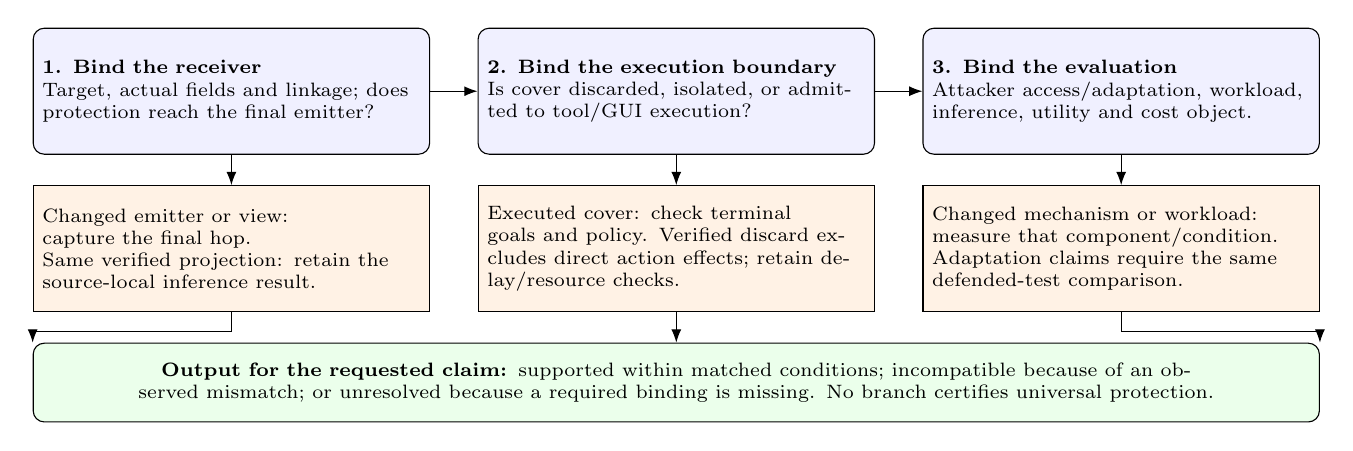
\begin{tikzpicture}[font=\scriptsize,>=Latex,
check/.style={draw,rounded corners,fill=blue!6,align=left,text width=4.8cm,minimum height=16mm},
test/.style={draw,fill=orange!10,align=left,text width=4.8cm,minimum height=16mm}]
\node[check] (receiver) at (0,0) {\textbf{1. Bind the receiver}\\Target, actual fields and linkage; does protection reach the final emitter?};
\node[check] (action) at (5.65,0) {\textbf{2. Bind the execution boundary}\\Is cover discarded, isolated, or admitted to tool/GUI execution?};
\node[check] (effect) at (11.3,0) {\textbf{3. Bind the evaluation}\\Attacker access/adaptation, workload, inference, utility and cost object.};
\draw[->] (receiver)--(action);
\draw[->] (action)--(effect);
\node[test] (rtest) at (0,-2.0) {Changed emitter or view:\\capture the final hop.\\Same verified projection: retain the source-local inference result.};
\node[test] (atest) at (5.65,-2.0) {Executed cover: check terminal goals and policy. Verified discard excludes direct action effects; retain delay/resource checks.};
\node[test] (etest) at (11.3,-2.0) {Changed mechanism or workload:\\measure that component/condition.\\Adaptation claims require the same defended-test comparison.};
\draw[->] (receiver)--(rtest);
\draw[->] (action)--(atest);
\draw[->] (effect)--(etest);
\node[draw,rounded corners,fill=green!8,align=center,text width=16.1cm,minimum height=10mm] (out) at (5.65,-3.7)
{\textbf{Output for the requested claim:} supported within matched conditions; incompatible because of an observed mismatch; or unresolved because a required binding is missing. No branch certifies universal protection.};
\draw[->] (rtest.south)--++(0,-.25)-|(out.north west);
\draw[->] (atest)--(out);
\draw[->] (etest.south)--++(0,-.25)-|(out.north east);
\end{tikzpicture}
\caption{Operational evidence-reuse checks.}\label{fig:defense-decision}\end{figure*}
\clearpage
\onecolumn
\section{Second-round transfer tests (E5--E7)}\label{app:transfer}
E5 and individual-attacker E6 results below retain the R2 measurements. Current E6/E7 suite summaries use post-review reanalysis in \path{experiments/sp2027-r3/}; historical registration and outputs remain in \path{experiments/sp2027-r2/}. A suite maximum is recomputed in each of 2,000 common task-bootstrap draws. Intervals condition on fixed out-of-fold predictions and omit retraining/search uncertainty. Meets: upper BA bound $<0.60$ and maximum point AUROC $<0.65$; Above: lower BA bound $>0.60$; otherwise inconclusive. This is a finite-suite criterion, not a security guarantee.
\begin{table*}[!ht]\centering\scriptsize
\caption{E5 per attacker with 95\% topic-bootstrap intervals (12 test topics). Wire: mean application-record bytes incl.\ 5-byte headers. Amb.: mean size of the nearest-sequence tie set.}
\begin{tabular}{@{}lllrrrrrrr@{}}\toprule
TLS & Target & Framing & Wire & $D_0$ total & $D_2$ total & $D_2$ count & $D_2$ sequence & ID & Amb.\\\midrule
1.2 & T1 & Buffered, unpadded & 721 & 100.0 [100.0,100.0] & 100.0 [100.0,100.0] & 100.0 [100.0,100.0] & 100.0 [100.0,100.0] & 87.5 & 1.3\\
1.2 & T1 & Buffered, training cap & 1570 & 50.0 [50.0,50.0] & 50.0 [50.0,50.0] & 50.0 [50.0,50.0] & 50.0 [50.0,50.0] & 2.1 & 48.0\\
1.2 & T1 & Stream, per token & 15038 & 100.0 [100.0,100.0] & 100.0 [100.0,100.0] & 100.0 [100.0,100.0] & 100.0 [100.0,100.0] & 100.0 & 1.0\\
1.2 & T1 & + random event pad & 19194 & 100.0 [100.0,100.0] & 100.0 [100.0,100.0] & 100.0 [100.0,100.0] & 100.0 [100.0,100.0] & 62.3 & 1.0\\
1.2 & T1 & + constant event size & 18255 & 100.0 [100.0,100.0] & 100.0 [100.0,100.0] & 100.0 [100.0,100.0] & 100.0 [100.0,100.0] & 58.3 & 2.3\\
1.2 & T1 & 8-token batches, const. & 3040 & 50.0 [50.0,50.0] & 100.0 [100.0,100.0] & 100.0 [100.0,100.0] & 100.0 [100.0,100.0] & 20.8 & 9.4\\
1.2 & T1 & Const.\ events + count cap & 36092 & 50.0 [50.0,50.0] & 50.0 [50.0,50.0] & 50.0 [50.0,50.0] & 50.0 [50.0,50.0] & 6.3 & 44.1\\
1.2 & T3 & Buffered, unpadded & 456 & 91.7 [79.2,100.0] & 91.7 [79.2,100.0] & 91.7 [79.2,100.0] & 91.7 [79.2,100.0] & 91.7 & 1.2\\
1.2 & T3 & Buffered, training cap & 635 & 50.0 [50.0,50.0] & 50.0 [50.0,50.0] & 50.0 [50.0,50.0] & 50.0 [50.0,50.0] & 4.2 & 44.2\\
1.2 & T3 & Stream, per token & 9713 & 87.5 [75.0,100.0] & 87.5 [75.0,100.0] & 87.5 [75.0,100.0] & 87.5 [75.0,100.0] & 100.0 & 1.0\\
1.2 & T3 & + random event pad & 12398 & 71.2 [58.3,83.8] & 87.9 [75.8,99.2] & 87.5 [75.0,100.0] & 87.9 [76.2,98.3] & 72.5 & 1.0\\
1.2 & T3 & + constant event size & 11803 & 79.2 [66.7,91.7] & 87.5 [75.0,100.0] & 87.5 [75.0,100.0] & 87.5 [75.0,100.0] & 70.8 & 1.8\\
1.2 & T3 & 8-token batches, const. & 2023 & 50.0 [50.0,50.0] & 87.5 [75.0,100.0] & 87.5 [75.0,100.0] & 87.5 [75.0,100.0] & 18.8 & 8.4\\
1.2 & T3 & Const.\ events + count cap & 15411 & 50.0 [50.0,50.0] & 50.0 [50.0,50.0] & 50.0 [50.0,50.0] & 50.0 [50.0,50.0] & 12.5 & 38.6\\
1.3 & T1 & Buffered, unpadded & 686 & 100.0 [100.0,100.0] & 100.0 [100.0,100.0] & 100.0 [100.0,100.0] & 100.0 [100.0,100.0] & 87.5 & 1.3\\
1.3 & T1 & Buffered, training cap & 1500 & 50.0 [50.0,50.0] & 50.0 [50.0,50.0] & 50.0 [50.0,50.0] & 50.0 [50.0,50.0] & 2.1 & 48.0\\
1.3 & T1 & Stream, per token & 14294 & 100.0 [100.0,100.0] & 100.0 [100.0,100.0] & 100.0 [100.0,100.0] & 100.0 [100.0,100.0] & 100.0 & 1.0\\
1.3 & T1 & + random event pad & 18450 & 100.0 [100.0,100.0] & 100.0 [100.0,100.0] & 100.0 [100.0,100.0] & 100.0 [100.0,100.0] & 62.3 & 1.0\\
1.3 & T1 & + constant event size & 17511 & 100.0 [100.0,100.0] & 100.0 [100.0,100.0] & 100.0 [100.0,100.0] & 100.0 [100.0,100.0] & 58.3 & 2.3\\
1.3 & T1 & 8-token batches, const. & 2938 & 50.0 [50.0,50.0] & 100.0 [100.0,100.0] & 100.0 [100.0,100.0] & 100.0 [100.0,100.0] & 20.8 & 9.4\\
1.3 & T1 & Const.\ events + count cap & 34626 & 50.0 [50.0,50.0] & 50.0 [50.0,50.0] & 50.0 [50.0,50.0] & 50.0 [50.0,50.0] & 6.3 & 44.1\\
1.3 & T3 & Buffered, unpadded & 433 & 91.7 [79.2,100.0] & 91.7 [79.2,100.0] & 91.7 [79.2,100.0] & 83.3 [70.8,95.8] & 91.7 & 1.2\\
1.3 & T3 & Buffered, training cap & 606 & 50.0 [50.0,50.0] & 50.0 [50.0,50.0] & 50.0 [50.0,50.0] & 50.0 [50.0,50.0] & 4.2 & 44.2\\
1.3 & T3 & Stream, per token & 9230 & 87.5 [75.0,100.0] & 87.5 [75.0,100.0] & 87.5 [75.0,100.0] & 87.5 [75.0,100.0] & 100.0 & 1.0\\
1.3 & T3 & + random event pad & 11915 & 68.8 [56.7,81.7] & 87.9 [75.8,99.2] & 87.5 [75.0,100.0] & 87.5 [75.4,98.3] & 72.5 & 1.0\\
1.3 & T3 & + constant event size & 11321 & 79.2 [66.7,91.7] & 87.5 [75.0,100.0] & 87.5 [75.0,100.0] & 87.5 [75.0,100.0] & 70.8 & 1.8\\
1.3 & T3 & 8-token batches, const. & 1953 & 50.0 [50.0,50.0] & 87.5 [75.0,100.0] & 87.5 [75.0,100.0] & 87.5 [75.0,100.0] & 18.8 & 8.4\\
1.3 & T3 & Const.\ events + count cap & 14782 & 50.0 [50.0,50.0] & 50.0 [50.0,50.0] & 50.0 [50.0,50.0] & 50.0 [50.0,50.0] & 12.5 & 38.6\\
\bottomrule\end{tabular}\end{table*}
\begin{table*}[!ht]\centering\scriptsize
\caption{E6 dispatch view: balanced accuracy (\%) with task-cluster bootstrap intervals (115 tasks, 3 seeds per task), best AUROC, active-account equality and cover-call error rate.}
\begin{tabular}{@{}llrrrrrrr@{}}\toprule
Target & Cover & $D_0$ GB & $D_2$ LR & $D_2$ GB & Count rule & AUROC & Acct.\ eq. & Cover err.\\\midrule
cancel & No cover & 100.0 [100.0,100.0] & 100.0 [100.0,100.0] & 100.0 [100.0,100.0] & 100.0 [100.0,100.0] & 1.00 & 100.0 & 0.0\\
cancel & Cancel, $p{=}0.5$ & 74.6 [71.6,77.4] & 84.5 [75.9,92.1] & 86.1 [78.4,93.9] & 83.3 [75.0,91.2] & 0.95 & 100.0 & 0.0\\
cancel & Cancel, $p{=}1$ & 50.0 [50.0,50.0] & 97.1 [92.4,100.0] & 100.0 [100.0,100.0] & 100.0 [100.0,100.0] & 1.00 & 100.0 & 0.0\\
cancel & Cancel, $p{=}1$, live execution & 50.0 [50.0,50.0] & 98.1 [95.4,100.0] & 100.0 [100.0,100.0] & 100.0 [100.0,100.0] & 1.00 & 100.0 & 0.0\\
cancel & Cancel count $\to 2$ & 50.0 [50.0,50.0] & 76.9 [64.8,88.0] & 69.4 [57.6,81.7] & 50.0 [50.0,50.0] & 0.85 & 100.0 & 2.8\\
cancel & One decoy program & 91.9 [89.8,94.2] & 68.1 [60.2,76.7] & 66.0 [60.1,72.2] & 91.9 [89.8,94.2] & 0.92 & 100.0 & 3.0\\
cancel & Two decoy programs & 83.5 [80.5,86.5] & 55.9 [48.4,63.6] & 57.0 [49.9,64.1] & 83.5 [80.5,86.5] & 0.86 & 100.0 & 4.3\\
cancel & Shape equalization & 50.0 [50.0,50.0] & 44.8 [37.6,52.4] & 49.2 [44.0,54.8] & 50.0 [50.0,50.0] & 0.50 & 100.0 & 5.7\\
return & No cover & 100.0 [100.0,100.0] & 97.8 [94.0,100.0] & 100.0 [100.0,100.0] & 100.0 [100.0,100.0] & 1.00 & 100.0 & 0.0\\
return & Cancel, $p{=}0.5$ & 100.0 [100.0,100.0] & 98.0 [94.3,100.0] & 100.0 [100.0,100.0] & 100.0 [100.0,100.0] & 1.00 & 100.0 & 0.0\\
return & Cancel, $p{=}1$ & 100.0 [100.0,100.0] & 97.5 [94.8,99.6] & 100.0 [100.0,100.0] & 100.0 [100.0,100.0] & 1.00 & 100.0 & 0.0\\
return & Cancel, $p{=}1$, live execution & 100.0 [100.0,100.0] & 98.0 [94.3,100.0] & 100.0 [100.0,100.0] & 100.0 [100.0,100.0] & 1.00 & 100.0 & 0.0\\
return & Cancel count $\to 2$ & 100.0 [100.0,100.0] & 98.0 [95.4,100.0] & 100.0 [100.0,100.0] & 100.0 [100.0,100.0] & 1.00 & 100.0 & 2.8\\
return & One decoy program & 85.9 [82.9,89.0] & 73.2 [66.6,79.5] & 71.1 [65.5,76.8] & 85.9 [82.9,89.0] & 0.88 & 100.0 & 3.0\\
return & Two decoy programs & 78.1 [75.0,81.2] & 70.6 [64.1,77.3] & 69.1 [62.9,75.0] & 78.1 [75.0,81.2] & 0.85 & 100.0 & 4.3\\
return & Shape equalization & 50.0 [50.0,50.0] & 54.5 [48.4,60.3] & 50.3 [45.4,55.5] & 50.0 [50.0,50.0] & 0.53 & 100.0 & 5.7\\
\bottomrule\end{tabular}\end{table*}

\begin{table*}[!ht]\centering\scriptsize
\caption{Corrected E6 suite maxima and task-bootstrap intervals. Individual-attacker results above are unchanged. AUROC is also maximized over the evaluated suite.}
\begin{tabular}{@{}llrrl@{}}\toprule
Target & Cover & Max BA [95\% CI] & Max AUROC & Criterion\\\midrule
cancel & No cover & 100.0 [100.0,100.0] & 1.00 & Above\\
cancel & Cancel, $p{=}0.5$ & 86.1 [80.9,94.2] & 0.95 & Above\\
cancel & Cancel, $p{=}1$ & 100.0 [100.0,100.0] & 1.00 & Above\\
cancel & Cancel, $p{=}1$, live & 100.0 [100.0,100.0] & 1.00 & Above\\
cancel & Cancel count $\to2$ & 76.9 [67.0,88.1] & 0.85 & Above\\
cancel & One decoy & 91.9 [89.8,94.2] & 0.92 & Above\\
cancel & Two decoys & 83.5 [80.5,86.5] & 0.86 & Above\\
cancel & Shape & 50.0 [50.0,54.8] & 0.50 & Meets\\
return & No cover & 100.0 [100.0,100.0] & 1.00 & Above\\
return & Cancel, $p{=}0.5$ & 100.0 [100.0,100.0] & 1.00 & Above\\
return & Cancel, $p{=}1$ & 100.0 [100.0,100.0] & 1.00 & Above\\
return & Cancel, $p{=}1$, live & 100.0 [100.0,100.0] & 1.00 & Above\\
return & Cancel count $\to2$ & 100.0 [100.0,100.0] & 1.00 & Above\\
return & One decoy & 85.9 [82.9,89.0] & 0.88 & Above\\
return & Two decoys & 78.1 [75.0,81.2] & 0.85 & Above\\
return & Shape & 54.5 [50.0,60.4] & 0.53 & Inconcl.\\
\bottomrule\end{tabular}\end{table*}

\begin{table*}[!ht]\centering\scriptsize
\caption{Corrected E7 suite maxima (4,140 saved TLS sessions). Decoder: held-out request/response size-to-tool accuracy; it differs from request-only identification. Costs use raw/no-cover as denominator. Defense calibration uses the full public task population.}
\begin{tabular}{@{}lllrrlrrr@{}}\toprule
Target & Framing & Cover & Max BA [95\% CI] & AUROC & Criterion & Decoder & Bytes$\times$ & Calls$\times$\\\midrule
cancel & raw & No cover & 100.0 [100.0,100.0] & 1.00 & Above & 92.8 & 1.00 & 1.00\\
cancel & raw & Cancel count $\to2$ & 72.7 [63.4,84.5] & 0.81 & Above & 94.7 & 1.38 & 1.35\\
cancel & raw & One decoy & 91.9 [89.8,94.2] & 0.92 & Above & 99.7 & 2.03 & 2.01\\
cancel & raw & Shape & 51.2 [50.0,58.8] & 0.54 & Meets & 100.0 & 7.56 & 7.71\\
cancel & bucket1024 & No cover & 60.1 [50.0,73.3] & 0.67 & Inconcl. & 35.2 & 2.42 & 1.00\\
cancel & bucket1024 & Cancel count $\to2$ & 67.5 [58.5,78.9] & 0.70 & Inconcl. & 33.5 & 3.25 & 1.35\\
cancel & bucket1024 & One decoy & 60.0 [53.4,68.7] & 0.59 & Inconcl. & 35.5 & 4.90 & 2.01\\
cancel & bucket1024 & Shape & 55.3 [52.2,63.6] & 0.59 & Inconcl. & 26.5 & 18.56 & 7.71\\
cancel & const & No cover & 59.7 [50.0,72.3] & 0.62 & Inconcl. & 30.4 & 3.41 & 1.00\\
cancel & const & Cancel count $\to2$ & 64.9 [54.9,76.7] & 0.66 & Inconcl. & 30.0 & 4.61 & 1.35\\
cancel & const & One decoy & 59.7 [52.6,67.4] & 0.59 & Inconcl. & 30.5 & 6.87 & 2.01\\
cancel & const & Shape & 54.4 [50.0,62.5] & 0.50 & Inconcl. & 21.6 & 26.32 & 7.71\\
return & raw & No cover & 95.7 [90.7,99.4] & 0.96 & Above & 93.8 & 1.00 & 1.00\\
return & raw & Cancel count $\to2$ & 95.7 [90.6,99.4] & 0.96 & Above & 95.4 & 1.38 & 1.35\\
return & raw & One decoy & 85.9 [82.9,89.0] & 0.88 & Above & 100.0 & 2.03 & 2.01\\
return & raw & Shape & 60.5 [54.9,66.4] & 0.61 & Inconcl. & 100.0 & 7.56 & 7.71\\
return & bucket1024 & No cover & 73.9 [66.6,83.1] & 0.76 & Above & 35.2 & 2.42 & 1.00\\
return & bucket1024 & Cancel count $\to2$ & 66.0 [59.8,75.8] & 0.70 & Inconcl. & 33.5 & 3.25 & 1.35\\
return & bucket1024 & One decoy & 59.1 [54.1,66.8] & 0.60 & Inconcl. & 35.5 & 4.90 & 2.01\\
return & bucket1024 & Shape & 50.6 [50.0,57.3] & 0.52 & Meets & 26.5 & 18.56 & 7.71\\
return & const & No cover & 53.6 [50.0,63.9] & 0.55 & Inconcl. & 30.4 & 3.41 & 1.00\\
return & const & Cancel count $\to2$ & 59.1 [52.3,68.6] & 0.61 & Inconcl. & 30.0 & 4.61 & 1.35\\
return & const & One decoy & 56.8 [51.4,63.6] & 0.57 & Inconcl. & 30.5 & 6.87 & 2.01\\
return & const & Shape & 50.0 [50.0,55.1] & 0.50 & Meets & 21.6 & 26.32 & 7.71\\
\bottomrule\end{tabular}\end{table*}

\begin{table*}[!ht]\centering\footnotesize
\caption{Request-only tool identification: training-fold size table, unseen-size fallback to the training majority. Each of 582 reference calls is tested once. The 95.7\% raw in-sample purity is excluded from held-out accuracy.}
\begin{tabular}{@{}llrr@{}}\toprule
Task stratification & Framing & Held-out accuracy (\%) & Training-majority baseline (\%)\\\midrule
cancel & raw & 89.9 & 29.4\\
cancel & bucket1024 & 29.4 & 29.4\\
cancel & const & 29.4 & 29.4\\
return & raw & 91.4 & 29.4\\
return & bucket1024 & 29.4 & 29.4\\
return & const & 29.4 & 29.4\\
\bottomrule\end{tabular}
\par\smallskip Training-only tool-count maxima overflow on five distinct held-out tasks (22, 28, 40, 67, 87) under either target split. This is a feasibility audit, not a rerun of defense efficacy. Full fold membership and overflow records are released. No tested network configuration meets the criterion for both targets.
\end{table*}

\begin{table}[t]\centering\footnotesize
\caption{E5: the same 48 saved responses emitted by a buffered or a token-streaming frontend (TLS~1.3 loopback captures). Bytes are relative to the unpadded emitter of the same kind. TTFB/Done: first and last delivered byte in token intervals (accounting proxy). Accuracies on 24 held-out outputs (12 topics); ID: closed-world top-1 identification among 48 responses (chance 2.1\%).}\label{tab:transfer-streaming}
\setlength{\tabcolsep}{1.6pt}
\begin{tabularx}{\columnwidth}{@{}Yrrrrrrr@{}}\toprule
 & & & & \multicolumn{2}{c}{T1 acc.} & T3 & \\\cmidrule(lr){5-6}\cmidrule(lr){7-7}
Emitter / framing & Bytes$\times$ & TTFB & Done & $D_0$ & $D_2$ & $D_2$ & ID\\\midrule
Buffered, unpadded & 1.00 & 105 & 105 & 100.0 & 100.0 & 91.7 & 87.5\\
Buffered, training cap & 2.19 & 105 & 105 & 50.0 & 50.0 & 50.0 & 2.1\\
Stream, per token & 1.00 & 1 & 105 & 100.0 & 100.0 & 87.5 & 100.0\\
+ random event pad & 1.29 & 1 & 105 & 100.0 & 100.0 & 87.9 & 62.3\\
+ constant event size & 1.23 & 1 & 105 & 100.0 & 100.0 & 87.5 & 58.3\\
8-token batches, const. & 0.21 & 8 & 105 & 50.0 & 100.0 & 87.5 & 20.8\\
Const.\ events + count cap & 2.42 & 1 & 208 & 50.0 & 50.0 & 50.0 & 6.3\\
\bottomrule\end{tabularx}
\par\smallskip\raggedright
$D_2$ is the best of total-byte threshold, record-count threshold and a logistic sequence model, each fitted on defended training outputs. Random padding: 10 socket-measured draws plus an independent profiling run. TLS~1.2 gives identical accuracies and byte ratios within 0.03. Tokens: o200k\_base proxy. Count cap: 208 (T1) and 88 (T3) events fitted on training outputs; 2/24 and 5/24 test outputs overflow it.
\end{table}

\begin{table*}[t]\centering\footnotesize
\caption{E6/E7: randomized cover on 115 retail reference programs $\times$ 3 seeds. Entries are the best held-out balanced accuracy (\%) over all attackers for the cancellation (C, 18 positive tasks) and return (R, 32) targets. Dispatch view: tool names and response lengths. Network view: TLS~1.2 record lengths on the agent--tool link under raw, 1024-byte bucket or constant framing.}\label{tab:transfer-cover}
\setlength{\tabcolsep}{3.5pt}
\begin{tabularx}{\textwidth}{@{}Yrrrrrrrrrrr@{}}\toprule
 & \multicolumn{4}{c}{Dispatch view (E6)} & \multicolumn{7}{c}{Network view (E7)}\\\cmidrule(lr){2-5}\cmidrule(lr){6-12}
 & & & & & \multicolumn{2}{c}{Raw} & \multicolumn{2}{c}{Bucket} & \multicolumn{2}{c}{Constant} & \\\cmidrule(lr){6-7}\cmidrule(lr){8-9}\cmidrule(lr){10-11}
Cover policy & C & R & Calls+ & DB eq. & C & R & C & R & C & R & Bytes$\times$\\\midrule
No cover & 100.0 & 100.0 & 0.00 & 100.0 & 100.0 & 95.7 & 60.1 & 73.9 & 59.7 & 53.6 & 3.4\\
Cancel, $p{=}0.5$ & 86.1 & 100.0 & 0.10 & 100.0 & --- & --- & --- & --- & --- & --- & ---\\
Cancel, $p{=}1$ & 100.0 & 100.0 & 0.20 & 100.0 & --- & --- & --- & --- & --- & --- & ---\\
Cancel, $p{=}1$, live execution & 100.0 & 100.0 & 0.20 & 0.0 & --- & --- & --- & --- & --- & --- & ---\\
Cancel count $\to 2$ & 76.9 & 100.0 & 0.35 & 100.0 & 72.7 & 95.7 & 67.5 & 66.0 & 64.9 & 59.1 & 4.6\\
One decoy program & 91.9 & 85.9 & 1.01 & 100.0 & 91.9 & 85.9 & 60.0 & 59.1 & 59.7 & 56.8 & 6.9\\
Two decoy programs & 83.5 & 78.1 & 1.98 & 100.0 & --- & --- & --- & --- & --- & --- & ---\\
Shape equalization & 50.0 & 54.5 & 6.71 & 100.0 & 51.2 & 60.5 & 55.3 & 50.6 & 54.4 & 50.0 & 26.3\\
\bottomrule\end{tabularx}
\par\smallskip\raggedright
Calls+: cover calls per real call. DB eq.: orders/users equal to reference. Cover is sampled from other users' reference programs and placed at random positions; all policies except ``live'' run cover in a per-session sandbox. Attackers: $D_0$/$D_2$ gradient boosting and logistic regression, a count rule and, on the network view, a size-profiling decoder; task-grouped 5-fold cross-validation. Bytes$\times$: constant framing relative to raw framing without cover. Suite-maximum intervals: Supplement S12. Defense templates/pools/caps use all 115 tasks; attacker fitting uses training folds. No network configuration meets the criterion for both targets.
\end{table*}

\begin{table*}[t]\centering\footnotesize
\caption{Current reassessment of the seven author-written judgments recorded before E5--E7. Historical outcome labels are preserved in the artifact, not counted as audit accuracy.}\label{tab:transfer-predictions}
\begin{tabularx}{\textwidth}{@{}lp{.27\textwidth}Y@{}}\toprule
ID & Claim under examination & Current evidence and qualification\\\midrule
P1 & Buffered cost transfers to a stream & Emitter mismatch supported: per-event padding leaves T1 at 100\%; constant-shape stream costs 2.42$\times$.\\
P2 & Low $D_0$ establishes protection & Counterexample supported: batching and cancellation cover give $D_0$ 50\%, $D_2$ 100\%.\\
P3 & Per-event padding prevents identification & Counterexample supported: top-1 58--62\% versus 2.1\% chance in the closed candidate set.\\
P4 & Equal cancellation count hides cancellation & Residual leakage supported: count rule 50\%; maximum BA 76.9\%.\\
P5 & Dispatch protection transfers to the tool link & Protected-source premise unmet: count/decoy policies already leak at dispatch. Network BA 72.7--95.7\% shows persistence.\\
P6 & Framing alone protects intent & Bucketed return remains above threshold; remaining framing-only cells inconclusive.\\
P7 & Joint cover/framing protects both targets & Not established: no configuration meets both target criteria. Joint constant framing: 50.0--54.4\% BA; 26.3$\times$ bytes, 7.7$\times$ calls.\\
\bottomrule\end{tabularx}
\end{table*}

\clearpage
\section{Stand-in planner pipeline (E8) and online cover}\label{app:e8}
\path{experiments/sp2027-r2/agent/} runs tool-calling agents and a user simulator on the 115 retail tasks, applies \emph{online} cover (decided before each real call from the history only, with a final flush) and replays every session over TLS. Because sandboxed cover and framing never reach the agent, one trajectory per task and seed serves all policies. No LLM was available for this revision; the rows below use stand-in planners and exercise the pipeline. The scripted planner replays reference programs (native reward 1.00); the noisy planner inserts extra reads before each reference call with probability 0.3 (7.2 versus 5.1 real calls per session). These are synthetic results, not agent measurements.
\begin{table*}[!ht]\centering\scriptsize
\caption{E8 diagnostics report point estimates only; no suite-maximum interval was recomputed for online runs. Current offline E6/E7 intervals are in S12. Best held-out balanced accuracy (\%) point estimates for offline versus online cover. Const.: constant framing on the agent--tool link. Calls+: cover calls per real call. Overflow: sessions whose real calls exceed the shape template or the cancellation target.}
\begin{tabular}{@{}llrrrrrr@{}}\toprule
Planner / cover timing & Cover & Dispatch C & Dispatch R & Const.\ C & Const.\ R & Calls+ & Overflow (\%)\\\midrule
Offline (E6/E7) & cancel const2 & 76.9 & 100.0 & 64.9 & 59.1 & 0.35 & 0.0\\
Offline (E6/E7) & decoy1 & 91.9 & 85.9 & 59.7 & 56.8 & 1.01 & 0.0\\
Offline (E6/E7) & shape eq & 50.0 & 54.5 & 54.4 & 50.0 & 6.71 & 0.0\\
\midrule
Online, scripted & cancel const2 & 79.6 & 100.0 & 63.0 & 59.1 & 0.36 & 3.8\\
Online, scripted & decoy1 & 92.3 & 88.6 & 51.2 & 56.3 & 0.98 & 0.0\\
Online, scripted & shape eq & 63.8 & 55.1 & 57.5 & 55.9 & 6.73 & 0.0\\
\midrule
Online, noisy scripted & cancel const2 & 79.1 & 100.0 & 66.0 & 60.0 & 0.25 & 4.1\\
Online, noisy scripted & decoy1 & 92.3 & 88.6 & 51.8 & 56.2 & 0.69 & 0.0\\
Online, noisy scripted & shape eq & 55.9 & 53.9 & 60.5 & 56.2 & 4.52 & 20.9\\
\bottomrule\end{tabular}\end{table*}

\par\noindent The preceding E8 rows and availability statement describe the historical stand-in study. S14 reports the subsequent real-model collection and training-only calibration.\par
\clearpage
\section{Complete Real-Agent Evaluation with Training-Only Calibration (E9)}\label{sec:r4}
\subsection{Cohort and execution}
All 690 episodes in the frozen protocol are complete: 115 tasks, two prompt arms and three repetition identifiers. The fixed split assigns 69 tasks from 29 customers to training (414 episodes) and 46 tasks from 24 disjoint customers to testing (276 episodes). Every test task has all six prompt/repetition cells, and all failures and handoffs remain in the analysis. Training finished before defense calibration was frozen and test inference began. This section updates the earlier 663-episode publication snapshot to the full cohort; the immutable snapshot and the previous manuscript remain available in the archived release. No model configuration, prompt, split or defense parameter changed for this completion.

GPT-6.1 Sol with low reasoning effort supplies the planner and a separate user simulator through Codex app-server. The planner receives the retail policy, public tool schemas, interaction history and actual sandbox observations, and emits one structured action at each step. Reference actions and reward targets are used only for scoring. Each decision has a fresh ephemeral context without host tools or a host environment. The harness executes decisions in the pinned public retail simulator, with a 30-step limit. Repetition identifiers are cache namespaces; provider random seeds, temperature and an immutable weight snapshot are unavailable.

\subsection{Prompts and defense calibration}
The baseline prompt is the retail policy. The rules prompt adds one customer-details read after identification and before order access, an order read before each order write, and avoidance of unnecessary repeated reads. It preserves authorization and task requirements and prohibits unrelated operations for hiding intent. Both arms are evaluated under raw transport, padding only, online shape cover only, and joint shape cover with constant framing.

Only training trajectories from both prompts determine shared per-tool count maxima, donor pools and size caps. Donor calls exclude the active customer. Request caps are the largest training request plus four bytes rounded to a 256-byte multiple; response caps use the training 95th percentile plus four bytes rounded to a 1024-byte multiple, including training donor responses. Frozen caps are 1,024 and 3,072 bytes. The online dispatcher uses only past real-call counts, inserts a shadow call with probability 0.6 when a deficit exists and flushes remaining deficits at episode end. Overflow calls pass through; oversize messages expand to a 1024-byte bucket. Test data never recalibrate these parameters.

Shadow calls execute on isolated cloned state; their observations are suppressed and real calls/responses pass through unchanged. For deterministic tools with no timing-dependent side effects, projecting away cover gives the same planner-visible history under all program conditions. The replay therefore isolates transport intervention on the same realized actions, with reward preserved by the isolation invariant. All 690 real-call projections agree across the 2,760 saved sessions. Online means scheduling from past calls; interactive wall-clock delay and shared-resource feedback remain outside this replay measurement. A byte-transparent relay captures actual serialized requests and sandbox responses over local TLS~1.2.

\subsection{Attackers and uncertainty}
The frozen suite includes a training-majority baseline, clean-trained gradient boosting, defense-trained logistic regression and gradient boosting, a dispatch count rule, and network size-decoding learners and rules. All fitted parameters, thresholds and decoder tables use training data only. Targets are cancellation and return intent from the reference task; native task reward is scored separately using final database equality and required response strings. Points weight tasks equally. Intervals use 2,000 common customer-cluster bootstrap draws, retaining each customer's tasks and repetitions together and recomputing the suite maximum in each draw. Intervals condition on fitted attackers. Prompt contrasts pair task/repetition identifiers, without assuming identical conversations or shared model randomness.


\begin{table}[ht]\centering\small
\caption{E9 dispatch view: maximum BA (\%) with 95\% interval and maximum AUROC across the fixed suite, on 138 test episodes per prompt. BA and AUROC are separate suite maxima.}
\begin{tabular}{@{}llrrrr@{}}\toprule
Prompt & Condition & Cancel BA [CI] & AUC & Return BA [CI] & AUC\\\midrule
baseline & Raw & 97.2 [90.0, 100.0] & 0.997 & 97.0 [88.9, 100.0] & 0.972\\
baseline & Padding only & 97.2 [90.0, 100.0] & 0.997 & 97.0 [88.9, 100.0] & 0.972\\
baseline & Shape only & 55.6 [50.0, 63.0] & 0.556 & 57.7 [50.0, 67.4] & 0.620\\
baseline & Joint & 55.6 [50.0, 63.0] & 0.556 & 57.7 [50.0, 67.4] & 0.620\\
rules & Raw & 97.2 [90.0, 100.0] & 0.972 & 97.0 [88.9, 100.0] & 0.970\\
rules & Padding only & 97.2 [90.0, 100.0] & 0.972 & 97.0 [88.9, 100.0] & 0.970\\
rules & Shape only & 56.5 [50.0, 68.3] & 0.655 & 64.7 [54.3, 77.4] & 0.693\\
rules & Joint & 56.5 [50.0, 68.3] & 0.655 & 64.7 [54.3, 77.4] & 0.693\\
\bottomrule\end{tabular}\end{table}

\begin{table}[ht]\centering\small
\caption{E9 network view: maximum BA (\%) with 95\% interval and maximum AUROC across the fixed suite, on 138 test episodes per prompt. BA and AUROC are separate suite maxima.}
\begin{tabular}{@{}llrrrr@{}}\toprule
Prompt & Condition & Cancel BA [CI] & AUC & Return BA [CI] & AUC\\\midrule
baseline & Raw & 97.2 [90.0, 100.0] & 0.993 & 94.0 [85.8, 100.0] & 0.948\\
baseline & Padding only & 66.1 [50.0, 83.9] & 0.634 & 55.5 [50.0, 73.0] & 0.567\\
baseline & Shape only & 60.8 [55.4, 71.3] & 0.657 & 51.9 [50.5, 57.8] & 0.579\\
baseline & Joint & 50.0 [50.0, 60.6] & 0.500 & 50.0 [50.0, 65.5] & 0.500\\
rules & Raw & 97.2 [90.0, 100.0] & 0.978 & 93.5 [85.0, 99.5] & 0.937\\
rules & Padding only & 67.6 [50.0, 85.0] & 0.636 & 57.9 [50.0, 78.9] & 0.548\\
rules & Shape only & 52.8 [50.0, 65.5] & 0.588 & 53.2 [50.4, 63.9] & 0.544\\
rules & Joint & 50.0 [50.0, 65.1] & 0.500 & 60.6 [50.0, 73.3] & 0.641\\
\bottomrule\end{tabular}\end{table}

\subsection{Utility, overhead and prompt contrasts}

\begin{table}[ht]\centering\small
\caption{Held-out utility and overhead. Reward and session overflow rates are percentages; ratios use raw transport within the same prompt.}
\begin{tabular}{@{}llrrrrrr@{}}\toprule
Prompt & Condition & Reward [CI] & Calls$\times$ & Bytes$\times$ & Count overflow & Cap overflow & Underfill\\\midrule
baseline & Raw & 79.7 [69.0, 89.7] & 1.00 & 1.00 & 0.0 & 0.0 & 0.0\\
baseline & Padding only & 79.7 [69.0, 89.7] & 1.00 & 4.02 & 0.0 & 6.5 & 0.0\\
baseline & Shape only & 79.7 [69.0, 89.7] & 3.83 & 4.16 & 38.4 & 0.0 & 0.0\\
baseline & Joint & 79.7 [69.0, 89.7] & 3.83 & 15.39 & 38.4 & 39.9 & 0.0\\
rules & Raw & 76.1 [63.3, 88.7] & 1.00 & 1.00 & 0.0 & 0.0 & 0.0\\
rules & Padding only & 76.1 [63.3, 88.7] & 1.00 & 4.04 & 0.0 & 6.5 & 0.0\\
rules & Shape only & 76.1 [63.3, 88.7] & 3.88 & 4.27 & 44.2 & 0.0 & 0.0\\
rules & Joint & 76.1 [63.3, 88.7] & 3.88 & 15.72 & 44.2 & 38.4 & 0.0\\
\bottomrule\end{tabular}\end{table}

Cancellation has 6 positive tasks from 5 customers; return has 11 positive tasks from 7 customers. Single-class draws excluded from 2,000 replicates: 6 for cancellation and 0 for return.

Baseline native reward is 110/138 (79.7\%); rules reward is 105/138 (76.1\%). All 24 baseline and 23 rules handoffs remain in the denominator. Joint-program cover-call error rates are 5.3\% and 5.0\%, respectively; all shape conditions have zero underfill. Overflow rates expose the resource demands of retaining real calls under the frozen training template.

\begin{table}[ht]\centering\small
\caption{Mechanical adherence to the two prompt-specified read-order rules (\% with customer-cluster interval).}
\begin{tabular}{@{}lrrr@{}}\toprule
Prompt & One successful customer read first & Order read before write & Both\\\midrule
baseline & 86.2 [74.5, 97.3] & 100.0 [100.0, 100.0] & 86.2 [74.5, 97.3]\\
rules & 97.1 [91.7, 100.0] & 100.0 [100.0, 100.0] & 97.1 [91.7, 100.0]\\
\bottomrule\end{tabular}\end{table}

\begin{table}[ht]\centering\small
\caption{Paired prompt contrasts using common customer-bootstrap draws.}
\begin{tabular}{@{}lr@{}}\toprule
Rules minus baseline & Difference [95\% CI], pp\\\midrule
Task reward & -3.6 [-9.5, 1.4]\\
Raw network, cancel BA & 0.0 [-8.3, 8.3]\\
Raw network, return BA & -0.5 [-2.6, 0.0]\\
Joint network, cancel BA & 0.0 [-1.7, 7.4]\\
Joint network, return BA & 10.6 [-13.3, 22.8]\\
\bottomrule\end{tabular}\end{table}

\begin{table}[ht]\centering\small
\caption{Post hoc paired program contrasts. The fixed attack suite is re-maximized under each condition within each common customer-bootstrap draw. Original predictions and the predeclared absolute criterion are unchanged.}
\begin{tabular}{@{}llr@{}}\toprule
Prompt & Target & Joint minus raw BA [95\% CI], pp\\\midrule
baseline & cancel & -47.2 [-50.0, -33.3]\\
baseline & return & -44.0 [-48.9, -27.8]\\
rules & cancel & -47.2 [-50.0, -26.0]\\
rules & return & -33.0 [-44.3, -18.9]\\
\bottomrule\end{tabular}\end{table}

\subsection{Interpretation and reproducibility}
The completed cohort shows strong raw-trace intent inference and a large reduction under joint transport intervention. Rules improve mechanical adherence to the two read-order rules while leaving network BA above 93\%. Baseline joint shaping reaches 50\% BA for both targets, reducing the raw scores by 47.2 and 44.0 points. The finite-suite criterion requires the BA interval upper bound below 60\% and point AUROC below 0.65. Baseline shape-only return meets it for that target; no condition meets it for both targets. Baseline joint upper bounds are 60.6\%/65.5\%, leaving the absolute-threshold conclusion inconclusive. The full-sample suite maximum equals the 50\% majority baseline; several fitted attacks make heterogeneous predictions whose customer-resampled BA can exceed 50\%. With only five cancellation-positive and seven return-positive customers, reselecting the maximum within each draw yields wider intervals. This mechanism does not imply a universal 10-point resolution floor or prove absence of residual population signal. The paired reduction intervals above exclude zero. Supplement S16 adds a task-permutation reference; the primary intervals remain clustered by customer. Rules-plus-joint return BA is 60.6\%; its rules-minus-baseline contrast includes zero, as does the reward contrast.

The evidence covers one public retail environment and one mutable model alias, which also supplies user simulation. All 115 tasks were available during prior project development. The formal customer holdout therefore provides internal evaluation; external independent replication, broader model/environment transfer, provider-traffic measurement and interactive feedback effects remain follow-up questions.

The full cohort contains 11,586 model decisions, 2,760 TLS sessions and 176 attack-prediction sets. The frozen verifier passed after training-only recalibration, sandbox state replay, cover reconstruction, TLS accounting, metric/interval recomputation and request-provenance checks. Additional checks bind all agent actions and dialogue to actual model outputs and re-score required response strings. Offline attacker refitting reproduces the saved results and predictions exactly.

\path{experiments/sp2027-r4-full-20261023/} supplies full results, predictions and captures, plus the 27 new episodes and model records needed to extend the immutable 663-run snapshot. The three separately reported snapshot test episodes join the 27 new ones to expand the primary test from 246 to 276. \texttt{reproduce.py --reanalyze} reconstructs the full cohort from the base archives and delta, reruns analysis and executes the original frozen verifier without invoking a model. \texttt{verify\_extension.py} checks decision alignment and provenance. The earlier snapshot, historical R2/R3 studies and pilot archives retain their original denominators and bytes.


\clearpage
\section{Cross-Fitting, Operating Points and Leakage Localization (E10--E12)}\label{sec:r5-supp}
This section preserves the original-suite results. The expanded 11-attack E10/E12 analyses in S21 supersede those attack maxima in the main paper; the original predictions remain available for direct comparison.
E10 retrospectively reuses the E9 defense design and attack suite under customer-grouped stratified 5-fold cross-fitting over all 690 completed episodes (115 tasks, 53 customers; 14 cancellation-positive and 18 return-positive customers). In each fold, the count template, donor pools, size caps and all attackers are fit only on the other folds. Out-of-fold predictions are pooled, and intervals use 2,000 customer-cluster bootstrap draws with the suite maximum recomputed per draw. The six analyzed configurations are specified in \path{r5lib.py}. E11 selects among them using inner customer folds of the 69 frozen training tasks only (rule in \path{e11_select.py}), then evaluates it on the 46 original test tasks. These analyses reuse an already analyzed cohort; only the original E9 protocol was frozen before test collection. E12 ablates undefended traces to locate the signal.

Records are computed with an analytic TLS~1.2 AES-GCM model (fragment plus 24 bytes, 16,384-byte fragments). The model is validated against all 2,760 socket captures of the completed cohort and 120 fresh loopback captures of new cross-fitted sessions. \path{verify_r5.py} also checks byte-identical reproduction of the E9 calibration, all sessions, and all 32 result cells of both the 660-run primary grid of the 663-run snapshot and the completed cohort. The same analysis on the 660-episode snapshot grid is retained in \path{snapshot-660/}; there the bucket point gives 50.6\%/51.6\% with upper bounds of 59.2\%/58.3\%. Cross-fitted templates use more training customers than E9 and are therefore larger, which raises call overhead (5.0$\times$ versus 3.8$\times$). A quantile template is a natural next operating point.

\begin{table*}[ht]\centering\footnotesize\setlength{\tabcolsep}{3pt}
\caption{E10 cross-fitted network view: all configurations and prompts. Core = R4 suite; Ext. adds random forest, $k$-NN and a forest size decoder. SA-AUC: sign-agnostic AUROC $\max(A,1-A)$.}
\begin{tabular}{@{}llrrrrrrr@{}}\toprule
Configuration & Prompt & Cancel core [CI] & Ext. & SA-AUC & Return core [CI] & Ext. & SA-AUC & Bytes$\times$/Calls$\times$\\\midrule
R4 point (all tools, constant) (padding only) & baseline & 68.1 [55.4, 78.9] & 68.1 & 0.63 & 67.1 [57.2, 77.0] & 67.1 & 0.63 & 3.9/1.0\\
R4 point (all tools, constant) & baseline & 60.5 [51.5, 70.5] & 60.5 & 0.59 & 52.1 [50.0, 60.3] & 52.7 & 0.63 & 19.8/5.0\\
R4 point (all tools, constant) (padding only) & rules & 64.4 [54.6, 75.8] & 64.4 & 0.60 & 63.3 [52.7, 74.2] & 63.3 & 0.63 & 3.9/1.0\\
R4 point (all tools, constant) & rules & 58.8 [50.0, 68.6] & 58.8 & 0.57 & 59.4 [50.5, 68.0] & 59.4 & 0.58 & 19.9/5.0\\
All tools, 1024-B buckets & baseline & 52.2 [50.0, 60.5] & 52.2 & 0.54 & 52.7 [50.0, 60.2] & 52.7 & 0.61 & 12.4/5.0\\
All tools, 1024-B buckets & rules & 53.4 [50.0, 60.6] & 53.4 & 0.57 & 50.7 [50.0, 57.3] & 52.4 & 0.56 & 12.4/5.0\\
All tools, constant, q80 cap & baseline & 56.5 [50.5, 66.6] & 56.5 & 0.55 & 60.2 [55.0, 66.0] & 60.2 & 0.61 & 15.2/5.0\\
All tools, constant, q80 cap & rules & 51.0 [50.0, 57.8] & 51.0 & 0.54 & 51.3 [50.0, 56.4] & 51.3 & 0.61 & 15.3/5.0\\
Writes only, constant & baseline & 53.5 [50.0, 65.8] & 56.1 & 0.60 & 56.1 [50.0, 67.4] & 56.1 & 0.63 & 11.3/2.9\\
Writes only, constant & rules & 62.6 [50.0, 74.4] & 62.6 & 0.60 & 57.6 [50.0, 68.2] & 57.6 & 0.58 & 11.4/2.9\\
Writes only, constant, q80 cap & baseline & 53.7 [50.0, 66.4] & 53.7 & 0.55 & 62.0 [51.2, 73.3] & 62.0 & 0.66 & 8.6/2.9\\
Writes only, constant, q80 cap & rules & 51.7 [50.0, 63.3] & 53.4 & 0.58 & 58.6 [50.0, 70.3] & 58.6 & 0.64 & 8.7/2.9\\
Writes only, 1024-B buckets & baseline & 56.4 [50.0, 66.5] & 56.4 & 0.55 & 58.1 [50.1, 68.6] & 59.7 & 0.66 & 6.9/2.9\\
Writes only, 1024-B buckets & rules & 52.6 [50.0, 63.8] & 52.6 & 0.60 & 58.7 [51.6, 69.6] & 58.7 & 0.59 & 7.0/2.9\\
\bottomrule\end{tabular}\end{table*}

\begin{table}[ht]\centering\small
\caption{E11 inner (training-fold) selection statistics. Eligible: all four inner network BAs $\le 60\%$.}
\begin{tabular}{@{}lrrrrrr@{}}\toprule
Configuration & C/base & R/base & C/rules & R/rules & Bytes$\times$ & Eligible\\\midrule
R4 point (all tools, constant) & 54.9 & 53.5 & 58.4 & 52.6 & 15.2 & yes\\
All tools, 1024-B buckets & 53.3 & 58.1 & 55.3 & 56.8 & 9.8 & yes\\
All tools, constant, q80 cap & 56.8 & 56.8 & 53.1 & 54.8 & 11.7 & yes\\
Writes only, constant & 67.1 & 50.0 & 77.9 & 57.2 & 9.4 & no\\
Writes only, constant, q80 cap & 71.1 & 64.9 & 67.5 & 71.6 & 7.1 & no\\
Writes only, 1024-B buckets & 56.7 & 67.4 & 53.7 & 64.8 & 5.9 & no\\
\bottomrule\end{tabular}\end{table}

\begin{table}[ht]\centering\small
\caption{E12 observer ablation on undefended traces, cross-fitted (core-suite BA, \%).}
\begin{tabular}{@{}lllrr@{}}\toprule
Observer & Prompt & View & Cancel & Return\\\midrule
full & baseline & dispatch & 91.7 & 93.8\\
full & baseline & network & 91.7 & 85.5\\
full & rules & dispatch & 90.7 & 93.8\\
full & rules & network & 90.7 & 85.5\\
no writes & baseline & dispatch & 53.1 & 65.7\\
no writes & baseline & network & 55.2 & 59.9\\
no writes & rules & dispatch & 60.8 & 66.2\\
no writes & rules & network & 55.2 & 59.6\\
writes only & baseline & dispatch & 91.7 & 93.8\\
writes only & baseline & network & 91.7 & 84.9\\
writes only & rules & dispatch & 90.7 & 93.8\\
writes only & rules & network & 90.7 & 84.1\\
\bottomrule\end{tabular}\end{table}

\noindent Rules-prompt homogenization: distinct read-only call sequences fall from 74 to 62 (entropy 5.63 to 5.37 bits), whereas state-changing sequences stay at 37 versus 36 (4.08 versus 4.09 bits).\par

\clearpage
\section{Conditional Task-Permutation Reference}

This post hoc diagnostic holds the fitted E9 attackers fixed and permutes labels over the 46 test tasks 2,000 times (seed 20261023), keeping each task\textquotesingle s three repetitions together. Each draw recomputes the attack-suite maximum. It characterizes a task-label exchangeability reference; it does not preserve dependencies among tasks belonging to one customer. Consequently, the tail fractions below are conditional reference values, not customer-valid population $p$-values or evidence of equivalence. The original customer-cluster intervals, paired contrasts and frozen absolute criterion remain the primary assessments.

\begin{table}[ht]\centering\footnotesize

\caption{All 32 E9 cells: observed maximum BA, permutation mean and 95th percentile (\%), conditional tail fraction $(1+\#\{T_b\ge T_{\rm obs}\})/2001$, and positive excess over the 95th percentile (percentage points).}

\begin{tabular}{@{}llllrrrrr@{}}\toprule

Prompt & View & Condition & Target & BA & Ref. mean & Ref. 95th & Tail & Excess\\\midrule

baseline & dispatch & Padding & cancel & 97.2 & 54.6 & 65.3 & 0.0005 & 31.9\\

baseline & network & Padding & cancel & 66.1 & 55.2 & 70.8 & 0.0755 & 0.0\\

baseline & dispatch & Padding & return & 97.0 & 54.1 & 65.1 & 0.0005 & 31.9\\

baseline & network & Padding & return & 55.5 & 56.2 & 67.4 & 0.4883 & 0.0\\

baseline & dispatch & Raw & cancel & 97.2 & 54.6 & 65.3 & 0.0005 & 31.9\\

baseline & network & Raw & cancel & 97.2 & 55.5 & 68.5 & 0.0005 & 28.7\\

baseline & dispatch & Raw & return & 97.0 & 54.1 & 65.1 & 0.0005 & 31.9\\

baseline & network & Raw & return & 94.0 & 55.3 & 65.4 & 0.0005 & 28.7\\

baseline & dispatch & Joint & cancel & 55.6 & 54.2 & 62.8 & 0.3048 & 0.0\\

baseline & network & Joint & cancel & 50.0 & 54.7 & 66.2 & 1.0000 & 0.0\\

baseline & dispatch & Joint & return & 57.7 & 53.0 & 58.7 & 0.1034 & 0.0\\

baseline & network & Joint & return & 50.0 & 54.1 & 62.6 & 1.0000 & 0.0\\

baseline & dispatch & Shape & cancel & 55.6 & 54.2 & 62.8 & 0.3048 & 0.0\\

baseline & network & Shape & cancel & 60.8 & 54.9 & 63.3 & 0.0870 & 0.0\\

baseline & dispatch & Shape & return & 57.7 & 53.0 & 58.7 & 0.1034 & 0.0\\

baseline & network & Shape & return & 51.9 & 54.3 & 60.4 & 0.7956 & 0.0\\

rules & dispatch & Padding & cancel & 97.2 & 54.6 & 68.5 & 0.0005 & 28.7\\

rules & network & Padding & cancel & 67.6 & 55.7 & 69.2 & 0.1034 & 0.0\\

rules & dispatch & Padding & return & 97.0 & 54.4 & 65.1 & 0.0005 & 31.9\\

rules & network & Padding & return & 57.9 & 55.6 & 67.2 & 0.3033 & 0.0\\

rules & dispatch & Raw & cancel & 97.2 & 54.6 & 68.5 & 0.0005 & 28.7\\

rules & network & Raw & cancel & 97.2 & 55.1 & 68.5 & 0.0005 & 28.7\\

rules & dispatch & Raw & return & 97.0 & 54.4 & 65.1 & 0.0005 & 31.9\\

rules & network & Raw & return & 93.5 & 55.6 & 65.8 & 0.0005 & 27.8\\

rules & dispatch & Joint & cancel & 56.5 & 53.2 & 59.7 & 0.1889 & 0.0\\

rules & network & Joint & cancel & 50.0 & 53.8 & 63.2 & 1.0000 & 0.0\\

rules & dispatch & Joint & return & 64.7 & 53.5 & 60.7 & 0.0115 & 4.0\\

rules & network & Joint & return & 60.6 & 54.1 & 60.6 & 0.0680 & 0.0\\

rules & dispatch & Shape & cancel & 56.5 & 53.2 & 59.7 & 0.1889 & 0.0\\

rules & network & Shape & cancel & 52.8 & 54.3 & 60.8 & 0.6122 & 0.0\\

rules & dispatch & Shape & return & 64.7 & 53.5 & 60.7 & 0.0115 & 4.0\\

rules & network & Shape & return & 53.2 & 54.6 & 59.6 & 0.7081 & 0.0\\

\bottomrule\end{tabular}\end{table}

The baseline raw network cells exceed the reference 95th percentiles (68.5\%/65.4\%), whereas baseline joint cells have no positive excess. This is consistent with the measured paired reductions; failure to exceed a reference threshold is not a population guarantee. The diagnostic uses saved predictions and makes its task-level exchangeability assumption explicit.

\clearpage
\twocolumn
\section{Shadow Cover: Deployment Paths and Observer Boundaries}\label{sec:shadow-deployment}
This section translates the measured isolation mechanism into deployment contracts. The evidence is the existing E6/E7 reference-program study and E9--E12 real-agent trajectory analysis. The three paths below are engineering designs grounded in existing API primitives; they have not been evaluated as production integrations.

\begin{table}[t]\centering\footnotesize
\caption{Deployment boundary: the relevant passive observer and what the measured mechanism can protect.}\label{tab:r7-deployment}
\begin{tabularx}{\columnwidth}{@{}p{.18\columnwidth}YY@{}}\toprule
Setting & Visible information & Applicability / trusted point\\\midrule
Same-host sidecar & Host trace/process/IPC metadata, if permitted & Link padding alone does not hide host instrumentation; isolate the monitor's access.\\
Same-VPC gateway & Ingress record sizes, times and addresses & Tunnel or shadow shaping can protect this link; gateway/markers remain trusted.\\
Remote SaaS/MCP & IP, unprotected SNI, per-endpoint flows and times & Shared ingress needed for tool-identity cover; ECH alone does not hide destination IP.\\
Cross-organization & Each hop's routing; provider calls/commit log & No guarantee across all hops. A trusted isolated executor is an explicit added assumption.\\\bottomrule
\end{tabularx}\end{table}


\subsection{What padding leaves visible, and what a tunnel changes}
E7's no-cover bucketed framing leaves return BA at 73.9\%. E9's baseline per-call padding leaves cancellation/return BA at 66.1\%/55.5\%. A padded request and response still contribute observable records: invocation count, direction changes and ordered turns remain available even if individual sizes coincide. The joint E9 intervention reduces the two measured BAs to 50.0\% by combining call-profile shaping with constant framing. This identifies a useful intervention boundary; it does not prove that executing dummy tools is necessary for every network threat model.

RFC~9347 describes a different construction: aggregate and fragment inner traffic into fixed-size ESP packets, send at a constant rate and use padding when no inner data is ready \cite{rfc9347}. For a passive observer of that tunnel alone, dummy transport traffic can conceal application call boundaries without reaching a tool. Protecting workflow duration also requires a common or otherwise workload-independent transmission horizon in both directions; destination choice, tunnel start/stop and congestion responses remain part of the observation contract. The E7/E9 per-call ablations do not measure this complete construction. E13 separately implements bidirectional fixed-cell TLS encapsulation with a training-sized horizon and measures its security/cost on the same live tool workload; it is not an IPsec implementation.

At the orchestrator-to-tool boundary, a multiparty relay may instead see decoded RPCs, tool names or forwarding events after a transport tunnel terminates. A tunnel's padding disappears at that point. Cover must survive to the relevant observer as plausible calls, or application fields must remain encrypted through the relay. E6/E9 evaluate the specified call-name/length and network projections. They do not establish indistinguishability against unrestricted argument inspection, routing logs or a tool provider's state view.

\subsection{Three execution paths}
\paragraph{1. Authorized reads and verified no-ops}
Where authorized read operations suffice for the protected observation, issue them against permitted live resources and discard their responses before the planner. This can avoid a replicated backend. The read-only decoy pattern is related to WRA \cite{jeong2026wra}; its ability to conceal write intent depends on what the observer sees. A receiver that recognizes write methods cannot be confused by adding only reads. E12 localizes operation-category information in the write-bearing profile; its action-defined labels do not establish leakage of unrelated attributes.

A no-op needs the invariant $f(s,a)=s$ for the designated protected state. Idempotence alone permits the first call to change state. Reads can also incur billing, access logs, cache changes or rate limits, so the adapter must specify its state scope and budget those effects. Cover selection must respect resource authorization and avoid exposing unrelated users' data. No claim about reads being the majority of production tool traffic is needed for this path.

\paragraph{2. Native noncommit and isolated test environments}
Kubernetes server-side dry-run performs admission and validation without persisting the resource; unsafe admission side effects cause rejection, and authorization matches the corresponding real request \cite{kubernetesdryrun}. This supplies a concrete noncommit primitive. Stripe sandboxes instead keep a separate test environment in which payments do not move real money \cite{stripesandboxes}. They instantiate isolated state, rather than a dry-run flag on a live payment. Neither feature alone establishes cover indistinguishability: an observer that reads the dry-run flag, test credential or separate destination can classify the call.

Database transactions can execute operations and then roll back their transactional updates \cite{postgresrollback}. This path is suitable only when relevant effects lie within the rollback contract. PostgreSQL sequence updates, for example, are not undone by transaction abort \cite{postgressequences}; locks, quotas and external effects also need explicit treatment. A rollback is not a general substitute for isolating irreversible remote actions. Common ingress framing must hide mode metadata from the intended observer, while the provider performing the operation remains trusted for that distinction.

\paragraph{3. A trusted gateway with isolated shadow endpoints}
A tool/MCP gateway can receive a common envelope containing an authenticated, encrypted real/cover marker. A fixed-length marker field is present in both modes and is readable only by the trusted gateway. It forwards real calls unchanged, routes cover writes to an isolated simulator and suppresses cover responses to the planner. The simulator can maintain only the state needed by supported operations; it need not clone an entire enterprise service. Error handling must fail closed: an unsupported shadow operation must never fall through to a live write.

This gives cover calls real local execution and real response packets, but does not automatically reproduce production latency or size distributions. A shared response scheduler and framing policy must normalize the exposed differences; their delay and resource costs need measurement. Retries, authentication failures, quota exhaustion and overflow must follow the same isolation contract. An encrypted marker alone is insufficient if a relay can infer the branch from destinations or correlate ingress calls with gateway-to-provider traffic.

\subsection{Where the protection ends}
The intended topology is an orchestrator, an optional forwarding relay, a trusted gateway, and separate live and shadow executors. Table~\ref{tab:shadow-boundary} distinguishes roles that are often conflated as a ``proxy.'' The trust requirement follows the ability to distinguish or commit the two branches, rather than organizational ownership alone.

\begin{table}[t]
\centering\footnotesize
\caption{Deployment contracts by observer. These are architectural conditions, not newly measured guarantees.}\label{tab:shadow-boundary}
\begin{tabularx}{\columnwidth}{@{}p{.24\columnwidth}Y@{}}
\toprule
Observer & Required protection boundary\\
\midrule
Passive ingress link & Joint call/size shaping or a complete transport tunnel; include timing and session horizon in the threat model.\\
Call-visible relay & Cover must reach it; marker, mode, routing and identifying arguments must be hidden or matched. E9 covers only its specified projection.\\
Trusted gateway & Reads the marker and routes branches; it is outside the protected observer set.\\
Downstream link & Ingress-only cover is insufficient if only real calls traverse this link; add protection on that link.\\
Tool provider & Sees live effects and mode/credentials; hiding committed intent requires additional assumptions beyond this design.\\
\bottomrule
\end{tabularx}
\end{table}

For a passive client-to-gateway observer, gateway-local cover can supply the measured kind of call-profile intervention. For an honest-but-curious relay, a protection claim additionally requires that its complete view exclude the discriminator and reveal no reliable substitute through arguments, timing or routing. A TLS-terminating relay that can read the marker does not satisfy this condition. The trusted gateway and the provider's commit log are not protected by moving cover into a local simulator.

All three paths preserve the logical planner transcript only when real observations pass unchanged and cover cannot affect live state or planner-visible feedback. That is the invariant checked in the existing replay. E13 adds local live-tool latency, failures, timing-aware attacks and complete tunnel controls at matched workload. Production quotas, WAN effects and fresh timing-dependent LLM interaction require deployment-specific evaluation. The contribution of shadow cover is a concrete way to shape an observable call profile while isolating its state effects, with an explicit choice of where that isolation must be enforced.

\clearpage
\section{Evidence Concordance and Evaluation Boundaries}\label{app:concordance}
\subsection{From families to result records}
The map has 82 families: 58 core and 24 adjacent. Ledger inclusion is an additional, result-level decision; it does not redefine core eligibility. All 20 audited mitigation families contribute 33 result records. Six contextual families contribute one record each, giving 26 families and 39 records. Multiple records separate mechanisms, execution modes or cost objects within a family. The 78 utility/cost field positions are two fields per result, not 78 independent experiments.

\begin{table}[!ht]\centering\footnotesize
\caption{Exact family-to-record reconciliation. Mitigation records total 33; contextual records total 6. Audit cells are 20 mitigation families $\times$ 9 items.}\label{tab:family-record-reconciliation}
\begin{tabularx}{\columnwidth}{@{}Yr@{}}\toprule
Family & Records\\\midrule
AHB~\cite{zhu2026turing} & 2\\
CachePrune~\cite{wu2026cacheprune} & 2\\
Cloud traffic benchmark~\cite{pouryousef2026traffic} & 2\\
Dangol workflow~\cite{dangol2026workflow} & 2\\
Early Bird~\cite{earlybird2025} & 2\\
I Know What You Said~\cite{gao2025iknow} & 1\\
KVGov~\cite{addagada2026kvgov} & 3\\
NetEcho~\cite{netecho2025} & 2\\
OTRO~\cite{lee2026otro} & 2\\
Remote timing~\cite{carlini2024remote} & 1\\
SafeKV~\cite{chu2025safekv} & 1\\
Shape and Substance~\cite{hadad2026shape} & 1\\
SparLeak~\cite{chen2026sparleak} & 1\\
Speculative decoding~\cite{wei2024speculation} & 1\\
SpliceLeak~\cite{spliceleak2026} & 2\\
TDXRay~\cite{hornetz2026tdxray} & 1\\
Time Will Tell~\cite{timewilltell2024} & 2\\
UI Traces~\cite{uitraces2026} & 1\\
Whisper Leak~\cite{whisperleak2025} & 3\\
WRA~\cite{jeong2026wra} & 1\\
\midrule\multicolumn{2}{l}{Contextual records (outside the 20-family audit)}\\
AgentTell~\cite{shahriar2026agenttell} & 1\\
Behind Bars~\cite{gu2026behindbars} & 1\\
FP-Agent~\cite{wang2026fpagent} & 1\\
LLMs Have Rhythm~\cite{alhazbi2025rhythm} & 1\\
ML privacy channels~\cite{debenedetti2024privacy} & 1\\
SIGLEAK~\cite{geng2026sigleak} & 1\\
\bottomrule\end{tabularx}\end{table}

The contextual record IDs are SIG-common-guardrail (SIGLEAK), AGENTTELL-fixed-instruction (AgentTell), FP-CLOUDFLARE (FP-Agent), BAR-co-running-noise (Behind Bars), RHYTHM-VPN (LLMs Have Rhythm), and DEB-filter-origin (ML privacy channels). Their roles are common-instruction residual leakage, fixed privacy instruction, access control, interference, generic VPN transport, and a privacy filter that creates an auxiliary signal. These contextual conditions do not constitute the audited confidentiality-mitigation claim.

The other 32 core families remain in the map: AgentPrint~\cite{agentprint2025}, AgentProv~\cite{wang2026agentprov}, ArchSnoop~\cite{weng2026archsnoop}, Cache contention~\cite{abubakar2026contention}, Campaign attribution~\cite{park2026crosscampaign}, ClawGuard~\cite{gan2026clawguard}, Cycle detection~\cite{george2025cycles}, Detokenization Leaks~\cite{weiss2026detokenization}, Edge EM leakage~\cite{alhalawani2026physicaledge}, Energon~\cite{chaudhuri2025energon}, InputSnatch~\cite{inputsnatch2024}, Leaky Language Models~\cite{majidi2026leakylms}, Lidar~\cite{wang2026lidar}, LLM-serving RCA~\cite{scheinert2026rca}, LLM-WFIN~\cite{jiao2025llmwfin}, LumiMAS~\cite{solomon2026lumimas}, MIRAGE~\cite{revankar2026mirage}, MoE prompt stealing~\cite{yona2024stealing}, MoEcho~\cite{ding2025moecho}, PAGE404~\cite{nazaraliyev2026page404}, PersonaFingerprint~\cite{song2026personafingerprint}, ProcGrep~\cite{oderinwale2026procgrep}, Prompt Echo~\cite{prompt_echo2026}, Prompt-cache audit~\cite{gu2025promptcaching}, PromptPeek~\cite{promptpeek2025}, Remote keylogging~\cite{weiss2024prompt}, Routing metadata~\cite{chen2026routingmetadata}, SparSEEty~\cite{jo2026sparseety}, Spill the Beans~\cite{spillbeans2025}, SplitDecoy~\cite{politis2026splitdecoy}, Web-agent unmasking~\cite{fayolle2026webagents}, Whose Agent?~\cite{kang2026whoseagent}. Their dispositions comprise 22 without a mitigation evaluation in the inspected scope, five authorized diagnostics, four unbound quantitative assertions, and SplitDecoy's distinct split-training boundary case. Thus absence from the result ledger does not imply exclusion from the SoK or that the family has no empirical evaluation. The artifact's family--record concordance gives the group, record IDs, source version and locators for every one of the 82 families.

\subsection{Experiment identifiers and manuscript locations}
The archived identifiers resolve protocols, predictions and verifiers. The appendix combines these components into one case study; the table maps the archived keys to their detailed accounts.
\begin{table}[!ht]\centering\footnotesize
\caption{Experiment concordance. Historical names are retained in code and data.}\label{tab:experiment-concordance}
\begin{tabularx}{\columnwidth}{@{}lYY@{}}\toprule
ID & Evidence / question & Current account\\\midrule
E1 & Two-link buffered transport; terminal caps & App. E; S9/S11\\
E2 & Saved finite-state tool plans; cover/state effects & S9; retail extension in S11\\
E3 & Clean versus defended fitting on buffered traces & App. E; S9/S11\\
E5 & Token-stream emitters & App. E; S12\\
E6 & Randomized dispatch cover & App. E; S12\\
E7 & Agent--tool TLS composition & App. E; S12\\
E8 & Scripted/noisy stand-in planners & S13; pipeline check\\
E9 & Real agents; pretest-frozen calibration & App. E; S14\\
E10/E12 & Cross-fitting and oracle localization & App. E; original suite S15, expanded suite S21\\
E11 & Retrospective operating-point selection & Main Appendix C; S15\\
E13 & Live tool timing, latency and complete tunnels & App. E; S19\\
E14 & Expanded attacks and classical WF adaptations & App. E; S20\\
E15 & Additional same-provider Luna trajectories & Main Appendix C; S22\\
E16 & Same-operation attribute diagnostic & Main Appendix C; S23.6\\
\bottomrule\end{tabularx}\end{table}

\subsection{Absolute thresholds and relative reductions}
The E9 suite criterion remains BA upper 95\% bound $<0.60$ and maximum AUROC $<0.65$. Joint shaping under the standard prompt has BA 50.0\%/50.0\%, with upper bounds 60.6\%/65.5\%; the absolute claim is inconclusive. The post hoc paired intervals support a reduction relative to undefended transport, not certification of this absolute target. With 24 held-out customers and only 5/7 positive customers, finite-cluster resampling and reselection of the suite maximum affect uncertainty. This is not a demonstrated universal bootstrap resolution floor or proof that the width is caused only by sample size. More repeats of the same customers do not supply new independent clusters.

The original-suite E10 bucketed standard-prompt upper bounds (60.5\%/60.2\%) do not meet the two-target absolute criterion; S21 reports the larger expanded-suite maxima and intervals retained in the case-study archive. Customer-grouped fitting avoids training/test mixing within a fold but remains retrospective reuse of the same cohort. E11's training-fold point-estimate selection rule is distinct from the E9 interval criterion; choosing a configuration under the former does not imply passing the latter. A future confirmatory cohort should freeze the defended policy, attacker suite, timing projection and cluster analysis before collection. Sample planning should vary independent positive and negative customers using explicit assumptions about heterogeneity and refitting, rather than infer guaranteed power from a near-chance point estimate.

\subsection{Timing evaluation: protocol and E13 coverage}
E7 and E9--E12 evaluate record sizes, directions and sequence order. They omit inter-arrival times, elapsed session duration and request service times. The end flush may form a detectable suffix; serial cover may delay responses, whereas concurrent cover may produce bursts. Logical planner-history equivalence excludes clocks, resource contention and timeout-dependent behavior. The observed byte/call ratios therefore cannot be read as measured interactive latency or timing-channel suppression.

The follow-up protocol calls for capturing timestamped ingress and egress traffic during live tool execution, with stable monotonic clock calibration, and measuring both serial and bounded-concurrency scheduling. Fit joint size/timing attackers, a flush/change-point segmenter and a real-versus-cover detector using only training customers. Keep the customer split, prompt arms and repeats together; evaluate the resulting intent BA/AUROC and paired changes on frozen test customers. Report timing-only, size/order-only and joint views, both with and without the flush suffix, including failures and timeouts.

At the same operating points, report first-response and episode p50/p95 latency, queueing, deadline violations, backend quotas, bytes/calls and native task reward. Compare per-call padding, full-profile cover, a paced/bounded-flush variant and a complete transport tunnel with a stated traffic horizon under matched workloads. Do not label synthetic delays or analytic service-time scenarios as measured production latency. E13 (S19) executes the local tool-chain portion of this specification, including observed TLS arrival timing, learned flush removal, serial/two-in-flight RPCs and complete fixed-rate tunnels. Fresh LLM replanning, WAN deployment, production quotas, an alternative paced-flush policy and a new customer cohort remain separate validation targets.

\clearpage
\onecolumn
\section{Live Tool Timing, Latency and Complete Tunnel Controls (E13)}\label{sec:r6-supp}
\subsection{Questions and measured boundary}
E13 executes the saved 690 real-agent action trajectories again through a live TLS tool server. It asks whether arrival timing restores intent inference after length/count shaping, whether an observer can identify the end flush or cover requests, and what actual waiting time accompanies each intervention. Six conditions yield 4,140 newly measured sessions. These are new tool executions and ciphertext arrival measurements, not new LLM generations or a new customer population.

The client driver waits for each real response before releasing its next saved action. The server invokes the pinned retail tool implementation against a live database clone; cover invokes the same implementation against a separate clone. Each real response is checked against the corresponding saved model observation, and the final live database is compared with unprotected execution of the same actions. This feedback-synchronized tool loop measures real queues and service times while holding the planner's action sequence fixed. Its clocks exclude LLM/user generation and WAN transit. No artificial read/write delay is injected. Reward preservation is inherited when all responses and final live state agree; it is not a new stochastic planner trial.

\subsection{Transport and execution controls}
All conditions use a fresh TLS~1.2 connection with ECDHE-RSA-AES128-GCM-SHA256 and TCP\_NODELAY through a byte-transparent loopback relay. The relay timestamps ciphertext chunk arrivals using a monotonic high-resolution clock and parses records; a record inherits the timestamp of its final observed chunk. The retained chunk log permits inspection of coalescing. These are relay-observed record times, not kernel packet timestamps. The application projection excludes handshakes and closure alerts. One session is measured at a time; episode and condition order are shuffled using a fixed seed.

The six conditions are raw transport, per-call constant framing, serial shadow cover with constant framing, the same cover with at most two outstanding RPCs, and two complete fixed-rate tunnel settings. The cover scheduler uses E9's frozen training donors, count template and random seed, observes only the executed prefix, and flushes remaining counts after the last real response. Real and shadow states have separate execution locks; neither a marker nor a shadow response is exposed to the passive link observer.

The tunnel fragments and reassembles the complete application stream. Both directions send a 4,096-byte plaintext cell at every slot, including when no payload is ready. An encrypted four-byte field gives the useful payload length; the remainder is padding. Dummy cells never invoke a tool. Every cell produces a 4,120-byte TLS ciphertext record, plus its five-byte header. This implements the fixed-size/constant-rate traffic-flow principle described by RFC~9347~\cite{rfc9347} over TLS; it is not an IPsec wire-format implementation.

The common service horizon is fixed using training messages only. For each training trajectory, sum the required request/response payload cells plus four slack cells per real call. The maximum budget, multiplied by 1.5 and rounded up with 16 additional slots, is lower-bounded by 128. This yields 133 slots: 266\,ms at 2\,ms per cell or 665\,ms at 5\,ms. Both directions continue through this horizon after the real workload completes. A horizon overflow is a retained failure, never a secret-dependent extension. The per-call framing caps use E9's frozen caps plus 256 bytes for the RPC envelope, with whole-cap overflow buckets. The operating points are fixed before test measurement.

Actual deadlines are rechecked against the measurement clock after sleeping; no ideal timestamps replace late sends or catch-up bursts. Both receivers must consume all 133 cells before closure. The saved outputs include cell deadlines, observed sends, pending queues and all requests/completions. A host scheduler and a local Python gateway remain part of this measured implementation. The two tunnel settings are fixed operating points, not an optimized cost frontier or a measurement of multi-session amortization.

\subsection{Attacks and fitting order}
The original customer-disjoint split is preserved: 414 training trajectories from 29 customers and 276 test trajectories from 24 customers. All 2,484 final training measurements precede attack fitting and a model-hash freeze; only then are the 1,656 final test sessions collected. An earlier complete development pass exposed two incomplete tunnel tails at connection closure. We added a receive-drain barrier, restored E9-style profilers to the attacker suite, and recollected the entire cohort; no individual test sessions were selectively replaced. Development records are archived separately. The original trajectories and labels were already known from E9, so this is a post hoc measurement study on the same population.

The intent suite has a training-majority baseline, balanced logistic regression ($C=1$), gradient boosting with 100 trees, and random forests with 200 trees and a minimum leaf size of two. Its three basic views are size/order, timing/direction and their joint features. Features include direction-specific count, size/gap quantiles, request/response size histograms, exchange-length vectors, duration, gap thresholds at 0.1/1/5/20\,ms, the first/last 32 positions, and largest-gap change-point summaries. For non-tunnel conditions, training-only size-to-tool profilers additionally feed a decoded gradient-boosting attacker and a training-selected count rule; these join both size/order and full-suite evaluations. At test time, all attackers consume observable records only. True tool names, RPC IDs, real/cover markers, true flush boundaries and internal execution times are excluded from test features.

Separate 80-tree forests (depth eight, minimum leaf size five) detect the flush suffix and real versus cover requests. Flush detection uses observable record neighborhoods and relative position/time; cover detection uses the same visible features at request-record positions. True execution annotations supply fitting/scoring labels only. For the flush-stripped intent view, training traces are transformed by three-fold customer-disjoint out-of-fold detectors. The full-training detector transforms test traces; a maximum-likelihood single transition estimates the cut. No oracle test boundary is used. The full adaptive suite unions every applicable view, allowing an observer to ignore timing or retain the unstripped trace.

\subsection{Inference, latency and reproducibility}
Intent intervals use 2,000 common customer-cluster bootstrap draws, retaining all tasks and repeats and recomputing the maximum over the suite in each draw. Paired differences reuse these draws. Draws lacking either target class have undefined BA/AUROC and are omitted from interval quantiles; their counts are archived. Intervals condition on fitted predictions and do not supply a new independent population estimate. The E9 absolute criterion remains unchanged: BA upper 95\% bound below 0.60 and AUROC below 0.65. Detector BA also uses customer clusters; detector AUROC is reported as a point estimate.

Latency is reported for individual real RPCs, the first real response, the last real response and the complete traffic window. Client scheduling queues, backend service, slot lateness and timeouts are retained separately. The descriptive count of real calls exceeding 100\,ms is a reference threshold, not a service-level guarantee. Byte ratios count measured application TLS records and their headers; call ratios count actual tool RPCs, excluding tunnel dummy cells. Source, calibration, model and capture hashes bind the analysis. The saved captures, fitted models and predictions support offline verification without new LLM or network requests.

\subsection{Findings across the measured boundaries}
For baseline prompts, serial cover's full-suite cancellation BA exceeds its size/order BA by 11.4 points [3.7,19.6]. The full-suite reduction relative to raw remains 30.3 points [23.1,37.6] for cancellation and 32.9 [19.9,40.7] for return. Thus the measurement supports a substantial reduction while exposing a residual clock signal. Flush and real/cover detectors pool both prompt arms: serial/parallel flush BA is 90.4\%/92.3\%, and cover BA is 82.5\%/96.1\%. Successful segmentation does not itself establish successful intent recovery; the separately fitted stripped-trace attacks test that transfer.

All 1,380 tunnel sessions contain exactly 133 records per direction with identical ciphertext lengths. Nevertheless, the measured directions can interleave differently, and scheduling is imperfect. In baseline-prompt tests, 2/5\,ms tunnel slot lateness has p95 1.88/1.68\,ms and maxima 282.6/307.5\,ms. These retained observations characterize the implementation, rather than an ideal zero-jitter clock. The full-suite baseline BAs are 62.5\%/52.9\% and 53.1\%/57.3\%; neither setting meets the two-target absolute criterion. Their 125.7$\times$ byte cost and one tool call per original action identify a different resource trade-off from shadow cover's 15.1$\times$ bytes and 3.83$\times$ calls. These fixed operating points do not establish an optimal tunnel or universal superiority of either mechanism.

No formal session fails, loses a real response, changes final live state or sends a cell before its deadline. Twelve of 2,000 cancellation bootstrap draws do not contain both target classes; all return draws are defined. The archived invalid-draw counters distinguish this finite-sample calculation issue from execution failures.

\subsection{Evaluation under WAN transit delay and jitter (Exp 4 Extension)}\label{sec:wan-netem-eval}
Local loopback measurement isolates backend execution and tool scheduling from transit variance, but real agent deployments operate over wide-area networks subject to packet propagation delays and jitter. To evaluate whether timing-based flush detection and intent inference hold outside the loopback environment, we extend Exp~4 with network emulation matching standard wide-area link profiles:
\begin{itemize}
    \item \textbf{WAN Mild}: 20\,ms one-way delay with 5\,ms normal jitter ($\sigma = 5$\,ms), representing regional cloud tool hosting ($40$\,ms nominal RTT).
    \item \textbf{WAN Realistic}: 50\,ms one-way delay with 10\,ms normal jitter ($\sigma = 10$\,ms), representing cross-region or transcontinental tool hosting ($100$\,ms nominal RTT).
\end{itemize}
The emulation runs directly in the bidirectional TLS transport relay using high-precision non-reordering FIFO delivery queues matching the behavior of Linux \texttt{tc netem}. Each real tool response across the WAN link gates the next action release, faithfully preserving feedback synchronization against live database clones. We repeat measurements on the complete set of 276 customer-held-out test episodes across both prompt arms (standard baseline and system-prompt rules), yielding 1,104 new TLS sessions per WAN profile (2,208 additional measured sessions total) across raw transport, per-call constant framing, serial shadow cover, and 2\,ms complete tunnels.

\paragraph{Resilience of flush detection}
Table~\ref{tab:wan-flush-comparison} assesses flush-phase detection across 15,278 ciphertext records from serial shadow cover sessions. We evaluate two attacker postures: (1) \emph{Direct Transfer}, where the attacker applies the frozen loopback detector $D_{\text{loop}}$ without network-specific recalibration, and (2) \emph{Adapted 5-Fold CV}, where the attacker refits the 80-tree random forest on customer-grouped training folds under the observed WAN network condition.

Under both WAN conditions, flush detection exhibits remarkable resilience. With direct transfer of $D_{\text{loop}}$, the detector achieves 89.4\% point BA (95\% CI [87.2\%, 91.7\%], AUROC 0.962) under 20\,ms/5\,ms jitter and 89.4\% point BA (95\% CI [87.3\%, 91.7\%], AUROC 0.963) under 50\,ms/10\,ms jitter, falling by only 1.0 percentage point from the loopback baseline (90.4\% BA, AUROC 0.967). Adapted retraining yields consistent performance (89.2\% and 89.0\% BA). This stability occurs because the flush phase transitions from feedback-gated tool intervals (punctuated by real database queries and network RTTs) to an un-gated burst of dummy requests. This macroscopic transition in inter-request density and duration creates a structural signature that easily cuts through 5--10\,ms transit noise.
\begin{table}[t]
\centering
\caption{Serial shadow cover flush-phase detection across network conditions (15,278 records from 276 test episodes). Direct transfer applies the frozen loopback detector $D_{\text{loop}}$; Adapted fits 5-fold customer-grouped models on the WAN workload.}
\label{tab:wan-flush-comparison}
\small
\begin{tabular}{lcccc}
\toprule
\textbf{Network Condition} & \textbf{Model} & \textbf{Flush Point BA} & \textbf{95\% CI} & \textbf{AUROC} \\
\midrule
Loopback (0 ms, 0 ms jitter) & Frozen $D_{\text{loop}}$ & 90.4\% & [88.3, 92.5] & 0.967 \\
\midrule
WAN Mild (20 ms, 5 ms jitter) & Transfer $D_{\text{loop}}$ & 89.4\% & [87.2, 91.7] & 0.962 \\
& Adapted $D_{\text{WAN}}$ & 89.2\% & [86.6, 91.5] & 0.958 \\
\midrule
WAN Realistic (50 ms, 10 ms jitter) & Transfer $D_{\text{loop}}$ & 89.4\% & [87.3, 91.7] & 0.963 \\
& Adapted $D_{\text{WAN}}$ & 89.0\% & [86.5, 91.3] & 0.958 \\
\bottomrule
\end{tabular}
\end{table}

\paragraph{Intent classification under transit jitter}
Table~\ref{tab:wan-controls-comparison} compares full-suite intent Balanced Accuracy across loopback and WAN conditions. For raw transport and per-call constant framing, intent classification is dominated by packet size and sequence order distributions, which are network-delay invariant; hence cancellation BA remains 91.7\% and 68.6\%, respectively.

For serial shadow cover, however, the timing signal exploited on loopback is substantially attenuated. On loopback, residual execution time differences allowed the full attack union to elevate cancellation BA to 61.4\% (11.4 points above size/order). Under WAN conditions, random transit jitter washes out microsecond-level tool service variations: cancellation BA falls to 50.0\% (exact chance level) under 20\,ms/5\,ms jitter and 54.0\% under 50\,ms/10\,ms jitter; return BA remains 50.7\% and 54.6\%. Thus, WAN network jitter acts as natural timing obfuscation against micro-timing intent inference, strengthening the intent-hiding property of serial cover while leaving macroscopic flush boundaries visible.

\paragraph{Operational limits: tunnel horizon exhaustion}
The WAN extension reveals a critical operational vulnerability in fixed-horizon tunnel designs. The 2\,ms full tunnel enforces a strict 133-slot horizon (266\,ms) sized against local loopback execution. On loopback, all 276 sessions successfully completed all tool calls within this window.

When executed over WAN links, each sequential tool RPC incurs network RTT. Under 20\,ms one-way delay (40\,ms RTT per call), tasks requiring multiple tool round-trips exhaust the 133 slots before their responses arrive; 191 out of 276 sessions (69.2\%) fail to complete due to horizon exhaustion (only 85/276 complete). Under 50\,ms delay (100\,ms RTT), horizon exhaustion surges to 98.2\% (271 out of 276 sessions fail; only 5 single-call sessions complete). This highlights an intrinsic deployment hazard: fixed-rate constant-bandwidth tunnels require worst-case horizon provisioning over WAN links, which would drastically multiply byte overhead (e.g., thousands of slots), or else suffer catastrophic protocol failure whenever network latency fluctuates.

In contrast, serial shadow cover and per-call constant framing adapt naturally to network delays: all 276 sessions complete successfully with 100\% response and database state equality across both WAN conditions. Their real-chain p95 latency expands predictably with network round-trips: from 26.2\,ms on loopback to 855.4\,ms under 20\,ms WAN and 1999.5\,ms under 50\,ms WAN.
\begin{table*}[t]
\centering
\caption{Timing defenses under loopback versus WAN conditions (276 test episodes). Full-suite intent Balanced Accuracy (BA) reported for cancellation / return. Incomplete/exhausted reflects sessions failing to complete all real calls within the fixed horizon.}
\label{tab:wan-controls-comparison}
\footnotesize\setlength{\tabcolsep}{3pt}
\begin{tabular}{lcccccc}
\toprule
\textbf{Condition} & \textbf{Network Environment} & \textbf{Full-Suite BA} & \textbf{Real p95 ms} & \textbf{Dur p95 ms} & \textbf{Byte Mult.} & \textbf{Status / Exh.} \\
\midrule
Raw transport & Loopback (0 ms, 0 ms jit.) & 91.7\% / 86.4\% & 15.4 & 15.5 & 1.0$\times$ & 276/276 \\
& WAN Mild (20 ms, 5 ms jit.) & 91.7\% / 86.4\% & 506.4 & 506.4 & 1.0$\times$ & 276/276 \\
& WAN Real. (50 ms, 10 ms jit.) & 91.7\% / 86.4\% & 1178.8 & 1178.8 & 1.0$\times$ & 276/276 \\
\midrule
Per-call constant framing & Loopback (0 ms, 0 ms jit.) & 68.6\% / 62.7\% & 16.6 & 16.7 & 3.9$\times$ & 276/276 \\
& WAN Mild (20 ms, 5 ms jit.) & 68.6\% / 54.8\% & 504.8 & 504.9 & 3.9$\times$ & 276/276 \\
& WAN Real. (50 ms, 10 ms jit.) & 68.6\% / 54.8\% & 1172.6 & 1172.6 & 3.9$\times$ & 276/276 \\
\midrule
Serial shadow cover & Loopback (0 ms, 0 ms jit.) & 61.4\% / 53.4\% & 26.2 & 46.6 & 15.1$\times$ & 276/276 \\
& WAN Mild (20 ms, 5 ms jit.) & 50.0\% / 50.7\% & 855.4 & 1314.9 & 15.3$\times$ & 276/276 \\
& WAN Real. (50 ms, 10 ms jit.) & 54.0\% / 54.6\% & 1999.5 & 3112.4 & 15.3$\times$ & 276/276 \\
\midrule
Full tunnel (2 ms cell) & Loopback (0 ms, 0 ms jit.) & 62.5\% / 52.9\% & 56.4 & 270.4 & 125.7$\times$ & 276/276 \\
& WAN Mild (20 ms, 5 ms jit.) & 54.4\% / 56.8\% & 286.7 & 291.6 & 127.0$\times$ & 85/276 \\
& WAN Real. (50 ms, 10 ms jit.) & 55.0\% / 52.6\% & 269.5 & 325.9 & 127.0$\times$ & 5/276 \\
\bottomrule
\end{tabular}
\end{table*}

\clearpage
\begin{table}[htbp]\centering\footnotesize
\caption{E13 baseline prompt: intent BA [95\% customer-cluster interval] and AUROC. The full suite unions all available views.}
\begin{tabular}{llrrrr}\toprule
Condition & View & Cancel BA [CI] & Return BA [CI] & Cancel AUC & Return AUC\\\midrule
Raw & Size/order & \mbox{91.7 [84.7, 100.0]} & \mbox{86.4 [79.5, 97.2]} & 0.917 & 0.875 \\
Raw & Timing/direction & \mbox{53.8 [50.0, 72.5]} & \mbox{52.9 [50.0, 64.1]} & 0.531 & 0.570 \\
Raw & Joint features & \mbox{84.3 [72.5, 97.4]} & \mbox{80.5 [69.9, 93.6]} & 0.836 & 0.835 \\
Raw & Full adaptive suite & \mbox{91.7 [84.7, 100.0]} & \mbox{86.4 [79.5, 97.2]} & 0.917 & 0.875 \\
\addlinespace[2pt]
Per-call padding & Size/order & \mbox{68.6 [50.0, 92.8]} & \mbox{54.8 [50.0, 74.8]} & 0.678 & 0.514 \\
Per-call padding & Timing/direction & \mbox{54.6 [50.0, 63.0]} & \mbox{62.7 [53.8, 78.0]} & 0.500 & 0.657 \\
Per-call padding & Joint features & \mbox{51.0 [50.0, 61.4]} & \mbox{50.2 [50.0, 69.0]} & 0.569 & 0.545 \\
Per-call padding & Full adaptive suite & \mbox{68.6 [50.8, 92.8]} & \mbox{62.7 [54.2, 79.3]} & 0.678 & 0.657 \\
\addlinespace[2pt]
Shadow, serial & Size/order & \mbox{50.0 [50.0, 56.9]} & \mbox{50.7 [50.0, 62.5]} & 0.500 & 0.505 \\
Shadow, serial & Timing/direction & \mbox{61.4 [53.8, 67.7]} & \mbox{52.9 [50.0, 62.5]} & 0.625 & 0.500 \\
Shadow, serial & Joint features & \mbox{51.0 [50.0, 64.6]} & \mbox{50.0 [50.0, 57.7]} & 0.596 & 0.500 \\
Shadow, serial & Estimated flush removed & \mbox{57.8 [50.0, 70.7]} & \mbox{53.4 [50.0, 64.6]} & 0.583 & 0.530 \\
Shadow, serial & Full adaptive suite & \mbox{61.4 [54.6, 71.1]} & \mbox{53.4 [50.0, 65.8]} & 0.625 & 0.530 \\
\addlinespace[2pt]
Shadow, two in flight & Size/order & \mbox{51.7 [50.0, 68.3]} & \mbox{57.7 [51.5, 66.1]} & 0.509 & 0.569 \\
Shadow, two in flight & Timing/direction & \mbox{50.0 [50.0, 57.1]} & \mbox{50.0 [50.0, 59.9]} & 0.554 & 0.500 \\
Shadow, two in flight & Joint features & \mbox{50.0 [50.0, 57.1]} & \mbox{52.6 [50.0, 63.3]} & 0.531 & 0.522 \\
Shadow, two in flight & Estimated flush removed & \mbox{50.0 [50.0, 64.0]} & \mbox{50.0 [50.0, 56.7]} & 0.500 & 0.500 \\
Shadow, two in flight & Full adaptive suite & \mbox{51.7 [50.0, 69.1]} & \mbox{57.7 [53.4, 66.8]} & 0.554 & 0.569 \\
\addlinespace[2pt]
Full tunnel, 2 ms & Size/order & \mbox{62.5 [54.3, 70.1]} & \mbox{52.9 [50.0, 61.0]} & 0.594 & 0.521 \\
Full tunnel, 2 ms & Timing/direction & \mbox{53.1 [50.2, 59.3]} & \mbox{50.0 [50.0, 55.6]} & 0.641 & 0.500 \\
Full tunnel, 2 ms & Joint features & \mbox{56.2 [50.9, 63.9]} & \mbox{50.0 [50.0, 57.4]} & 0.656 & 0.569 \\
Full tunnel, 2 ms & Full adaptive suite & \mbox{62.5 [55.6, 70.2]} & \mbox{52.9 [50.1, 61.3]} & 0.656 & 0.569 \\
\addlinespace[2pt]
Full tunnel, 5 ms & Size/order & \mbox{51.4 [50.0, 59.0]} & \mbox{54.5 [50.0, 60.3]} & 0.500 & 0.513 \\
Full tunnel, 5 ms & Timing/direction & \mbox{53.1 [50.0, 71.9]} & \mbox{53.2 [50.0, 62.4]} & 0.575 & 0.548 \\
Full tunnel, 5 ms & Joint features & \mbox{52.4 [50.0, 61.8]} & \mbox{57.3 [53.1, 63.7]} & 0.534 & 0.555 \\
Full tunnel, 5 ms & Full adaptive suite & \mbox{53.1 [50.3, 71.9]} & \mbox{57.3 [54.2, 64.2]} & 0.575 & 0.555 \\
\addlinespace[2pt]
\bottomrule\end{tabular}
\end{table}
\clearpage
\begin{table}[htbp]\centering\footnotesize
\caption{E13 rules prompt: intent BA [95\% customer-cluster interval] and AUROC. The full suite unions all available views.}
\begin{tabular}{llrrrr}\toprule
Condition & View & Cancel BA [CI] & Return BA [CI] & Cancel AUC & Return AUC\\\midrule
Raw & Size/order & \mbox{94.4 [83.3, 100.0]} & \mbox{87.0 [78.0, 97.6]} & 0.944 & 0.905 \\
Raw & Timing/direction & \mbox{57.8 [50.0, 70.6]} & \mbox{56.1 [50.0, 63.9]} & 0.598 & 0.557 \\
Raw & Joint features & \mbox{84.7 [75.2, 98.2]} & \mbox{79.1 [67.8, 92.0]} & 0.851 & 0.822 \\
Raw & Full adaptive suite & \mbox{94.4 [83.3, 100.0]} & \mbox{87.0 [78.0, 97.6]} & 0.944 & 0.905 \\
\addlinespace[2pt]
Per-call padding & Size/order & \mbox{70.1 [50.0, 86.0]} & \mbox{54.8 [50.0, 74.7]} & 0.680 & 0.500 \\
Per-call padding & Timing/direction & \mbox{55.8 [50.0, 70.2]} & \mbox{50.6 [50.0, 62.4]} & 0.530 & 0.534 \\
Per-call padding & Joint features & \mbox{59.4 [50.0, 76.6]} & \mbox{53.6 [50.0, 71.0]} & 0.575 & 0.508 \\
Per-call padding & Full adaptive suite & \mbox{70.1 [50.0, 86.0]} & \mbox{54.8 [50.0, 74.8]} & 0.680 & 0.534 \\
\addlinespace[2pt]
Shadow, serial & Size/order & \mbox{58.2 [50.2, 71.2]} & \mbox{57.9 [50.7, 66.8]} & 0.581 & 0.597 \\
Shadow, serial & Timing/direction & \mbox{51.5 [50.0, 69.8]} & \mbox{57.7 [52.3, 68.8]} & 0.500 & 0.560 \\
Shadow, serial & Joint features & \mbox{51.1 [50.0, 64.4]} & \mbox{55.1 [52.2, 65.3]} & 0.519 & 0.555 \\
Shadow, serial & Estimated flush removed & \mbox{50.1 [50.0, 55.6]} & \mbox{60.7 [50.8, 70.9]} & 0.500 & 0.622 \\
Shadow, serial & Full adaptive suite & \mbox{58.2 [52.9, 72.2]} & \mbox{60.7 [56.3, 71.7]} & 0.581 & 0.622 \\
\addlinespace[2pt]
Shadow, two in flight & Size/order & \mbox{54.7 [50.0, 66.7]} & \mbox{60.2 [50.5, 73.8]} & 0.580 & 0.576 \\
Shadow, two in flight & Timing/direction & \mbox{50.0 [50.0, 57.8]} & \mbox{54.0 [50.0, 62.6]} & 0.556 & 0.585 \\
Shadow, two in flight & Joint features & \mbox{55.3 [50.0, 67.1]} & \mbox{52.3 [50.0, 61.0]} & 0.578 & 0.546 \\
Shadow, two in flight & Estimated flush removed & \mbox{50.8 [50.0, 61.7]} & \mbox{54.0 [50.0, 67.0]} & 0.541 & 0.528 \\
Shadow, two in flight & Full adaptive suite & \mbox{55.3 [50.8, 68.2]} & \mbox{60.2 [54.5, 73.9]} & 0.580 & 0.585 \\
\addlinespace[2pt]
Full tunnel, 2 ms & Size/order & \mbox{51.5 [50.0, 65.0]} & \mbox{53.7 [50.0, 59.7]} & 0.500 & 0.500 \\
Full tunnel, 2 ms & Timing/direction & \mbox{53.1 [50.0, 64.2]} & \mbox{53.1 [50.0, 60.9]} & 0.500 & 0.563 \\
Full tunnel, 2 ms & Joint features & \mbox{51.5 [50.0, 58.1]} & \mbox{59.1 [52.2, 66.1]} & 0.500 & 0.590 \\
Full tunnel, 2 ms & Full adaptive suite & \mbox{53.1 [50.0, 65.6]} & \mbox{59.1 [52.8, 66.1]} & 0.500 & 0.590 \\
\addlinespace[2pt]
Full tunnel, 5 ms & Size/order & \mbox{50.0 [50.0, 53.6]} & \mbox{55.4 [50.9, 62.7]} & 0.500 & 0.549 \\
Full tunnel, 5 ms & Timing/direction & \mbox{50.0 [50.0, 50.4]} & \mbox{56.3 [51.0, 61.6]} & 0.500 & 0.530 \\
Full tunnel, 5 ms & Joint features & \mbox{50.0 [50.0, 57.5]} & \mbox{52.3 [50.0, 59.5]} & 0.500 & 0.534 \\
Full tunnel, 5 ms & Full adaptive suite & \mbox{50.0 [50.0, 57.5]} & \mbox{56.3 [55.0, 63.3]} & 0.500 & 0.549 \\
\addlinespace[2pt]
\bottomrule\end{tabular}
\end{table}
\clearpage
\begin{table}[htbp]\centering\footnotesize
\caption{E13 live execution costs, both prompt arms. Medians and 95th percentiles describe observed local RPCs; they are not production-service latency estimates.}
\begin{tabular}{llrrrrrr}\toprule
Prompt & Condition & Bytes$\times$ & Calls$\times$ & First p50/p95 & Last real p50/p95 & Traffic p50/p95 & RPC p50/p95\\\midrule
baseline & Raw & 1.00 & 1.00 & 2.3/3.4 & 8.8/15.4 & 8.8/15.5 & 1.0/1.8\\
baseline & Per-call padding & 3.92 & 1.00 & 2.3/3.7 & 8.5/16.6 & 8.5/16.7 & 1.0/1.8\\
baseline & Shadow, serial & 15.11 & 3.83 & 3.0/5.0 & 12.5/26.2 & 27.8/46.6 & 0.9/1.7\\
baseline & Shadow, two in flight & 15.11 & 3.83 & 2.7/4.5 & 11.3/20.8 & 23.6/37.4 & 1.2/2.4\\
baseline & Full tunnel, 2 ms & 125.71 & 1.00 & 5.4/11.2 & 30.9/56.4 & 267.0/270.4 & 4.0/6.2\\
baseline & Full tunnel, 5 ms & 125.71 & 1.00 & 11.3/12.4 & 71.4/112.3 & 666.1/666.6 & 10.0/10.9\\
rules & Raw & 1.00 & 1.00 & 2.2/3.7 & 8.1/15.7 & 8.2/15.7 & 1.0/1.7\\
rules & Per-call padding & 3.95 & 1.00 & 2.2/3.6 & 8.4/15.5 & 8.4/15.5 & 1.0/1.8\\
rules & Shadow, serial & 15.47 & 3.88 & 3.0/5.2 & 12.7/23.9 & 28.9/41.8 & 1.0/1.7\\
rules & Shadow, two in flight & 15.47 & 3.88 & 2.7/4.4 & 11.1/20.7 & 23.8/36.5 & 1.2/2.4\\
rules & Full tunnel, 2 ms & 128.38 & 1.00 & 5.4/7.7 & 29.8/48.8 & 267.0/267.9 & 4.0/5.8\\
rules & Full tunnel, 5 ms & 128.38 & 1.00 & 11.1/12.4 & 69.5/112.9 & 666.2/666.6 & 10.0/11.0\\
\bottomrule\end{tabular}
\par\smallskip All time columns are milliseconds. The saved results additionally report queue/service times, a descriptive 100 ms per-call deadline count, cell lateness, failures, and paired mean last-response differences.
\end{table}
\begin{table}[htbp]\centering\footnotesize
\caption{E13 learned timing/shape detectors on held-out customers, pooling both prompt arms. Flush labels identify records after the online flush declaration; cover labels identify encrypted requests. Ground truth is used only for fitting/scoring, never as an attacker feature.}
\begin{tabular}{llrrr}\toprule
Condition & Detector & BA [95\% CI] & AUROC & Records/requests\\\midrule
Shadow, serial & flush & \mbox{90.4 [88.3, 92.5]} & 0.967 & 15278 \\
Shadow, serial & cover & \mbox{82.5 [80.3, 84.7]} & 0.898 & 7639 \\
Shadow, two in flight & flush & \mbox{92.3 [90.6, 93.9]} & 0.979 & 15278 \\
Shadow, two in flight & cover & \mbox{96.1 [95.4, 96.7]} & 0.995 & 7639 \\
\bottomrule\end{tabular}
\end{table}


\clearpage
\section{Stronger Attackers, Classical Traffic Controls and Power Planning (E14)}\label{sec:r7-supp}
E14 is a post hoc sensitivity analysis of the existing cohort. It reuses E13's six measured conditions and adds seven offline transformations of its undefended captures, all on the same 414 training and 276 test trajectories. No new customer, model decision or packet measurement is produced by these transformations. The configuration and source hashes were frozen before fitting the new attacks; the source cohort and its earlier outcomes were already known. All configurations are reported.

\subsection{Defense-aware attacker expansion}
The primary attacker is $D_2$: it knows the algorithm and parameter distribution and fits on training examples generated under the evaluated defense. Seven R7 models comprise a majority control, logistic regression, gradient boosting, random forest, extra trees, a k-FP-style forest-leaf nearest-neighbor attack \cite{hayes2016kfp}, and a trainable 1D-CNN. This leaf adaptation uses 200 trees and Hamming-distance three-nearest-neighbor voting on training leaf fingerprints, not an exact reproduction of the original k-FP extractor. Tabular inputs contain full-trace counts, sizes, time summaries, directional bursts and sampled cumulative signed sizes. None includes tool names, labels, customer IDs, real/cover markers or test outcomes. The CNN uses direction, log length, log interarrival and a mask; its two convolutional layers have 16/32 channels, followed by mean/max pooling and a binary head. It is trained for 50 fixed epochs with Adam, learning rate .001 and class-weighted loss. The first/last halves of sequences longer than 512 records are retained; Table~\ref{tab:r7-all} reports truncation. Other learners preserve full-trace aggregate counts. Models and hashes are saved before test scoring. No test-guided hyperparameter selection is performed in this extension.

For measured conditions, the entire original E13 union remains included: size/order, timing, joint, training-derived profile decoding and learned flush stripping. The maximum therefore cannot decrease merely because a weaker new learner replaces an old one. Each of 2,000 common customer-bootstrap draws reselects the maximum. Draws missing a target class are excluded (counts are saved per cell). The intervals condition on fitted predictions and are not bounds against arbitrary future attackers. No expanded cell meets the original absolute criterion; the threshold is unchanged.

\subsection{Classical WF mechanisms adapted to RPC traces}
Every offline adapter tracks abstract fragments derived from input record sizes and verifies no loss, reordering or scheduling before release. This checks metadata and byte accounting, not payload-content equality or actual delivery. Fixed cells use 512 plaintext bytes plus 24 TLS~1.2 AEAD bytes and the five-byte header. Fragment IDs are excluded from attack inputs. All controls use the same held-out trajectories and byte accounting; they are not Tor deployments and do not inherit a published implementation's accuracy or guarantees.

Tamaraw uses constant per-direction slots, 40/12\,ms or 4/1.2\,ms, and randomized geometric padding to multiples of 50 cells \cite{cai2014systematic}. Input-order queueing propagates waits to subsequent real fragments. FRONT draws a uniform dummy budget and a Rayleigh schedule per direction and cancels outstanding dummies when the real trace ends \cite{gong2020front}; the budget is the training median cell count and the window spans training-duration quartiles. The shifted calibration fits those values only on the shorter half of training customers; D2 attackers still use all defended training customers and every test customer remains included. This is an in-population calibration stress test, not evidence of cross-environment transfer.

The WTF-PAD mechanism adaptation retains send/receive triggers, burst/gap/wait states, token removal/refill and infinity outcomes \cite{juarez2016wtfpad}. It uses an empirical training interarrival histogram, burst/gap infinity probabilities .1/.25, real-event reset and a 64-dummy-per-gap cap, rather than reproducing the public simulator's fitted log-normal Tor configuration. Walkie-Talkie molds half-duplex burst lengths with a random training donor from another customer and adds donor-only tail bursts \cite{wang2017walkietalkie}. It has no sensitive/non-sensitive symmetric pairing oracle and therefore does not inherit that pairing's indistinguishability argument. These exact adaptations and their limits are documented with the executable source.

\subsection{Results and cost interpretation}
The strongest learner depends on the operating point: the new CNN increases some tunnel BAs and supports inference on several classical controls; the forest-leaf attack improves the record-bucket return attack. The serial-shadow timing signal remains, so the earlier clock-boundary finding survives this expansion. The alternative WF points can reduce byte/tool-call cost substantially, precluding a claim that shadow cover is universally superior. The shorter-calibration FRONT result does not degrade monotonically: all points and both prompt arms are retained rather than selecting the direction expected by the hypothesis.

\begin{longtable}{@{}llrrrr@{}}
\caption{E14: all prompt/defense cells, maximum over the expanded attack suite. Customer bootstrap 95\% BA intervals; AUC is suite-maximum AUROC. All 52 cells fail the absolute criterion.}\label{tab:r7-all}\\
\toprule Prompt / condition & Target & BA [95\% CI] & AUC & Attacks & CNN trunc.\\\midrule\endfirsthead
\toprule Prompt / condition & Target & BA [95\% CI] & AUC & Attacks & CNN trunc.\\\midrule\endhead
Standard / Undefended & cancel & 91.7 [84.7, 100.0] & 0.917 & 19 & 0\\
Standard / Undefended & return & 86.4 [79.5, 97.2] & 0.875 & 19 & 0\\
Standard / Per-call constant & cancel & 68.6 [51.4, 92.8] & 0.678 & 19 & 0\\
Standard / Per-call constant & return & 62.7 [54.2, 79.5] & 0.657 & 19 & 0\\
Standard / Serial shadow & cancel & 61.4 [54.6, 71.4] & 0.625 & 22 & 0\\
Standard / Serial shadow & return & 53.4 [50.3, 65.8] & 0.530 & 22 & 0\\
Standard / Two-in-flight shadow & cancel & 51.7 [50.0, 69.1] & 0.554 & 22 & 0\\
Standard / Two-in-flight shadow & return & 57.7 [56.6, 69.7] & 0.596 & 22 & 0\\
Standard / Full tunnel, 2 ms & cancel & 62.5 [57.6, 70.2] & 0.708 & 17 & 0\\
Standard / Full tunnel, 2 ms & return & 55.2 [51.9, 62.0] & 0.569 & 17 & 0\\
Standard / Full tunnel, 5 ms & cancel & 54.6 [51.4, 72.9] & 0.618 & 17 & 0\\
Standard / Full tunnel, 5 ms & return & 57.3 [54.2, 64.2] & 0.555 & 17 & 0\\
Standard / Record buckets & cancel & 53.1 [50.0, 78.5] & 0.510 & 7 & 0\\
Standard / Record buckets & return & 69.8 [50.0, 86.9] & 0.689 & 7 & 0\\
Standard / Tamaraw 40/12 ms & cancel & 55.3 [50.0, 68.7] & 0.590 & 7 & 2\\
Standard / Tamaraw 40/12 ms & return & 55.3 [51.1, 64.4] & 0.594 & 7 & 2\\
Standard / Tamaraw 4/1.2 ms & cancel & 57.8 [50.0, 71.8] & 0.609 & 7 & 1\\
Standard / Tamaraw 4/1.2 ms & return & 51.8 [50.0, 61.8] & 0.525 & 7 & 1\\
Standard / FRONT & cancel & 59.0 [50.0, 69.9] & 0.623 & 7 & 0\\
Standard / FRONT & return & 69.3 [58.3, 81.8] & 0.713 & 7 & 0\\
Standard / WTF-PAD adaptation & cancel & 51.9 [50.0, 64.1] & 0.560 & 7 & 0\\
Standard / WTF-PAD adaptation & return & 62.7 [50.0, 79.6] & 0.635 & 7 & 0\\
Standard / WT random-donor & cancel & 50.0 [50.0, 67.0] & 0.526 & 7 & 0\\
Standard / WT random-donor & return & 56.7 [51.7, 67.8] & 0.607 & 7 & 0\\
Standard / FRONT, short calibration & cancel & 52.4 [50.0, 61.3] & 0.546 & 7 & 0\\
Standard / FRONT, short calibration & return & 56.0 [50.0, 71.1] & 0.618 & 7 & 0\\
Rules / Undefended & cancel & 94.4 [83.3, 100.0] & 0.944 & 19 & 0\\
Rules / Undefended & return & 87.0 [78.4, 97.6] & 0.905 & 19 & 0\\
Rules / Per-call constant & cancel & 70.1 [50.0, 86.0] & 0.680 & 19 & 0\\
Rules / Per-call constant & return & 61.9 [50.8, 78.0] & 0.563 & 19 & 0\\
Rules / Serial shadow & cancel & 58.2 [53.8, 76.3] & 0.589 & 22 & 0\\
Rules / Serial shadow & return & 60.7 [57.1, 72.6] & 0.626 & 22 & 0\\
Rules / Two-in-flight shadow & cancel & 56.9 [51.9, 70.4] & 0.580 & 22 & 0\\
Rules / Two-in-flight shadow & return & 60.2 [55.4, 73.9] & 0.639 & 22 & 0\\
Rules / Full tunnel, 2 ms & cancel & 53.1 [51.7, 65.7] & 0.504 & 17 & 0\\
Rules / Full tunnel, 2 ms & return & 59.1 [55.3, 67.6] & 0.590 & 17 & 0\\
Rules / Full tunnel, 5 ms & cancel & 58.3 [50.0, 67.9] & 0.539 & 17 & 0\\
Rules / Full tunnel, 5 ms & return & 56.3 [55.7, 64.0] & 0.595 & 17 & 0\\
Rules / Record buckets & cancel & 56.7 [50.0, 81.2] & 0.615 & 7 & 0\\
Rules / Record buckets & return & 70.8 [51.2, 88.0] & 0.703 & 7 & 0\\
Rules / Tamaraw 40/12 ms & cancel & 58.6 [56.3, 70.8] & 0.622 & 7 & 0\\
Rules / Tamaraw 40/12 ms & return & 50.0 [50.0, 60.3] & 0.500 & 7 & 0\\
Rules / Tamaraw 4/1.2 ms & cancel & 52.5 [50.0, 61.6] & 0.505 & 7 & 3\\
Rules / Tamaraw 4/1.2 ms & return & 54.6 [51.4, 61.5] & 0.534 & 7 & 3\\
Rules / FRONT & cancel & 58.5 [50.0, 69.6] & 0.544 & 7 & 0\\
Rules / FRONT & return & 60.4 [50.0, 75.1] & 0.635 & 7 & 0\\
Rules / WTF-PAD adaptation & cancel & 57.2 [50.0, 74.2] & 0.559 & 7 & 0\\
Rules / WTF-PAD adaptation & return & 61.0 [50.0, 77.6] & 0.625 & 7 & 0\\
Rules / WT random-donor & cancel & 51.4 [50.0, 68.8] & 0.606 & 7 & 0\\
Rules / WT random-donor & return & 56.3 [50.0, 66.6] & 0.558 & 7 & 0\\
Rules / FRONT, short calibration & cancel & 51.2 [50.0, 70.1] & 0.501 & 7 & 0\\
Rules / FRONT, short calibration & return & 62.9 [50.0, 77.2] & 0.655 & 7 & 0\\
\bottomrule\end{longtable}


\subsection{Matched-suite cost sensitivity}
The strongest-available union contains 17--22 attacks for measured conditions and seven for offline controls. Maxima over these unequal unions cannot by themselves establish a matched-attacker dominance relation. We therefore recompute all cells using exactly the seven common R7 models, without new fitting (Table~\ref{tab:r7-common}). Figure~\ref{fig:r7-pareto} uses this matched subset; its gray upper endpoints retain the larger available unions. For example, standard-prompt serial shadow changes from 61.4/53.4\% under its full union to 50.0/52.9\% under the common subset, while WT remains 50.0/56.7\%. WT's lower byte cost then trades off against higher worst-target BA, rather than dominating serial shadow. The serial timing finding from the full suite remains unchanged. One subset cell (standard-prompt, two-in-flight shadow, cancellation) meets the gate, but its full-union cell does not; restricting the comparison suite does not certify the defense. This sensitivity separates matched cost comparisons from the strongest observed attack evidence.
\begin{longtable}{@{}llrrrr@{}}
\caption{Matched-suite sensitivity: the same seven R7 models in every E14 condition. BA and AUROC maxima are independently reselected in every customer-bootstrap draw. This subset is used for the cost plot, not to replace the stronger available attack union or its absolute assessment.}\label{tab:r7-common}\\
\toprule Prompt / condition & Target & BA [95\% CI] & AUROC & Valid draws & Subset gate\\\midrule\endfirsthead
\toprule Prompt / condition & Target & BA [95\% CI] & AUROC & Valid draws & Subset gate\\\midrule\endhead
Standard / Undefended & cancel & 84.3 [72.7, 97.4] & 0.836 & 1988 & Unmet\\
Standard / Undefended & return & 76.9 [62.2, 90.4] & 0.828 & 2000 & Unmet\\
Standard / Per-call constant & cancel & 53.2 [50.0, 69.5] & 0.604 & 1988 & Unmet\\
Standard / Per-call constant & return & 59.1 [50.0, 73.8] & 0.656 & 2000 & Unmet\\
Standard / Serial shadow & cancel & 50.0 [50.0, 65.0] & 0.548 & 1988 & Unmet\\
Standard / Serial shadow & return & 52.9 [50.0, 60.3] & 0.526 & 2000 & Unmet\\
Standard / Two-in-flight shadow & cancel & 50.0 [50.0, 59.7] & 0.500 & 1988 & Pass\\
Standard / Two-in-flight shadow & return & 57.3 [55.0, 69.2] & 0.596 & 2000 & Unmet\\
Standard / Full tunnel, 2 ms & cancel & 59.9 [54.6, 67.3] & 0.708 & 1988 & Unmet\\
Standard / Full tunnel, 2 ms & return & 55.2 [50.1, 61.0] & 0.567 & 2000 & Unmet\\
Standard / Full tunnel, 5 ms & cancel & 54.6 [50.0, 70.5] & 0.618 & 1988 & Unmet\\
Standard / Full tunnel, 5 ms & return & 53.7 [51.3, 61.2] & 0.551 & 2000 & Unmet\\
Standard / Record buckets & cancel & 53.1 [50.0, 78.5] & 0.510 & 1988 & Unmet\\
Standard / Record buckets & return & 69.8 [50.0, 86.9] & 0.689 & 2000 & Unmet\\
Standard / Tamaraw 40/12 ms & cancel & 55.3 [50.0, 68.7] & 0.590 & 1988 & Unmet\\
Standard / Tamaraw 40/12 ms & return & 55.3 [51.1, 64.4] & 0.594 & 2000 & Unmet\\
Standard / Tamaraw 4/1.2 ms & cancel & 57.8 [50.0, 71.8] & 0.609 & 1988 & Unmet\\
Standard / Tamaraw 4/1.2 ms & return & 51.8 [50.0, 61.8] & 0.525 & 2000 & Unmet\\
Standard / FRONT & cancel & 59.0 [50.0, 69.9] & 0.623 & 1988 & Unmet\\
Standard / FRONT & return & 69.3 [58.3, 81.8] & 0.713 & 2000 & Unmet\\
Standard / WTF-PAD adaptation & cancel & 51.9 [50.0, 64.1] & 0.560 & 1988 & Unmet\\
Standard / WTF-PAD adaptation & return & 62.7 [50.0, 79.6] & 0.635 & 2000 & Unmet\\
Standard / WT random-donor & cancel & 50.0 [50.0, 67.0] & 0.526 & 1988 & Unmet\\
Standard / WT random-donor & return & 56.7 [51.7, 67.8] & 0.607 & 2000 & Unmet\\
Standard / FRONT, short calibration & cancel & 52.4 [50.0, 61.3] & 0.546 & 1988 & Unmet\\
Standard / FRONT, short calibration & return & 56.0 [50.0, 71.1] & 0.618 & 2000 & Unmet\\
Rules / Undefended & cancel & 84.7 [75.2, 98.5] & 0.851 & 1988 & Unmet\\
Rules / Undefended & return & 78.3 [63.3, 92.2] & 0.818 & 2000 & Unmet\\
Rules / Per-call constant & cancel & 59.4 [50.0, 77.5] & 0.594 & 1988 & Unmet\\
Rules / Per-call constant & return & 61.9 [50.0, 77.4] & 0.563 & 2000 & Unmet\\
Rules / Serial shadow & cancel & 56.1 [50.0, 76.2] & 0.589 & 1988 & Unmet\\
Rules / Serial shadow & return & 59.8 [53.8, 69.4] & 0.626 & 2000 & Unmet\\
Rules / Two-in-flight shadow & cancel & 56.9 [50.0, 69.2] & 0.566 & 1988 & Unmet\\
Rules / Two-in-flight shadow & return & 57.1 [53.8, 67.9] & 0.639 & 2000 & Unmet\\
Rules / Full tunnel, 2 ms & cancel & 52.8 [51.2, 61.6] & 0.504 & 1988 & Unmet\\
Rules / Full tunnel, 2 ms & return & 55.3 [51.7, 66.2] & 0.577 & 2000 & Unmet\\
Rules / Full tunnel, 5 ms & cancel & 58.3 [50.0, 67.9] & 0.539 & 1988 & Unmet\\
Rules / Full tunnel, 5 ms & return & 54.3 [51.6, 62.6] & 0.595 & 2000 & Unmet\\
Rules / Record buckets & cancel & 56.7 [50.0, 81.2] & 0.615 & 1988 & Unmet\\
Rules / Record buckets & return & 70.8 [51.2, 88.0] & 0.703 & 2000 & Unmet\\
Rules / Tamaraw 40/12 ms & cancel & 58.6 [56.3, 70.8] & 0.622 & 1988 & Unmet\\
Rules / Tamaraw 40/12 ms & return & 50.0 [50.0, 60.3] & 0.500 & 2000 & Unmet\\
Rules / Tamaraw 4/1.2 ms & cancel & 52.5 [50.0, 61.6] & 0.505 & 1988 & Unmet\\
Rules / Tamaraw 4/1.2 ms & return & 54.6 [51.4, 61.5] & 0.534 & 2000 & Unmet\\
Rules / FRONT & cancel & 58.5 [50.0, 69.6] & 0.544 & 1988 & Unmet\\
Rules / FRONT & return & 60.4 [50.0, 75.1] & 0.635 & 2000 & Unmet\\
Rules / WTF-PAD adaptation & cancel & 57.2 [50.0, 74.2] & 0.559 & 1988 & Unmet\\
Rules / WTF-PAD adaptation & return & 61.0 [50.0, 77.6] & 0.625 & 2000 & Unmet\\
Rules / WT random-donor & cancel & 51.4 [50.0, 68.8] & 0.606 & 1988 & Unmet\\
Rules / WT random-donor & return & 56.3 [50.0, 66.6] & 0.558 & 2000 & Unmet\\
Rules / FRONT, short calibration & cancel & 51.2 [50.0, 70.1] & 0.501 & 1988 & Unmet\\
Rules / FRONT, short calibration & return & 62.9 [50.0, 77.2] & 0.655 & 2000 & Unmet\\
\bottomrule\end{longtable}

\begin{figure}[p]\centering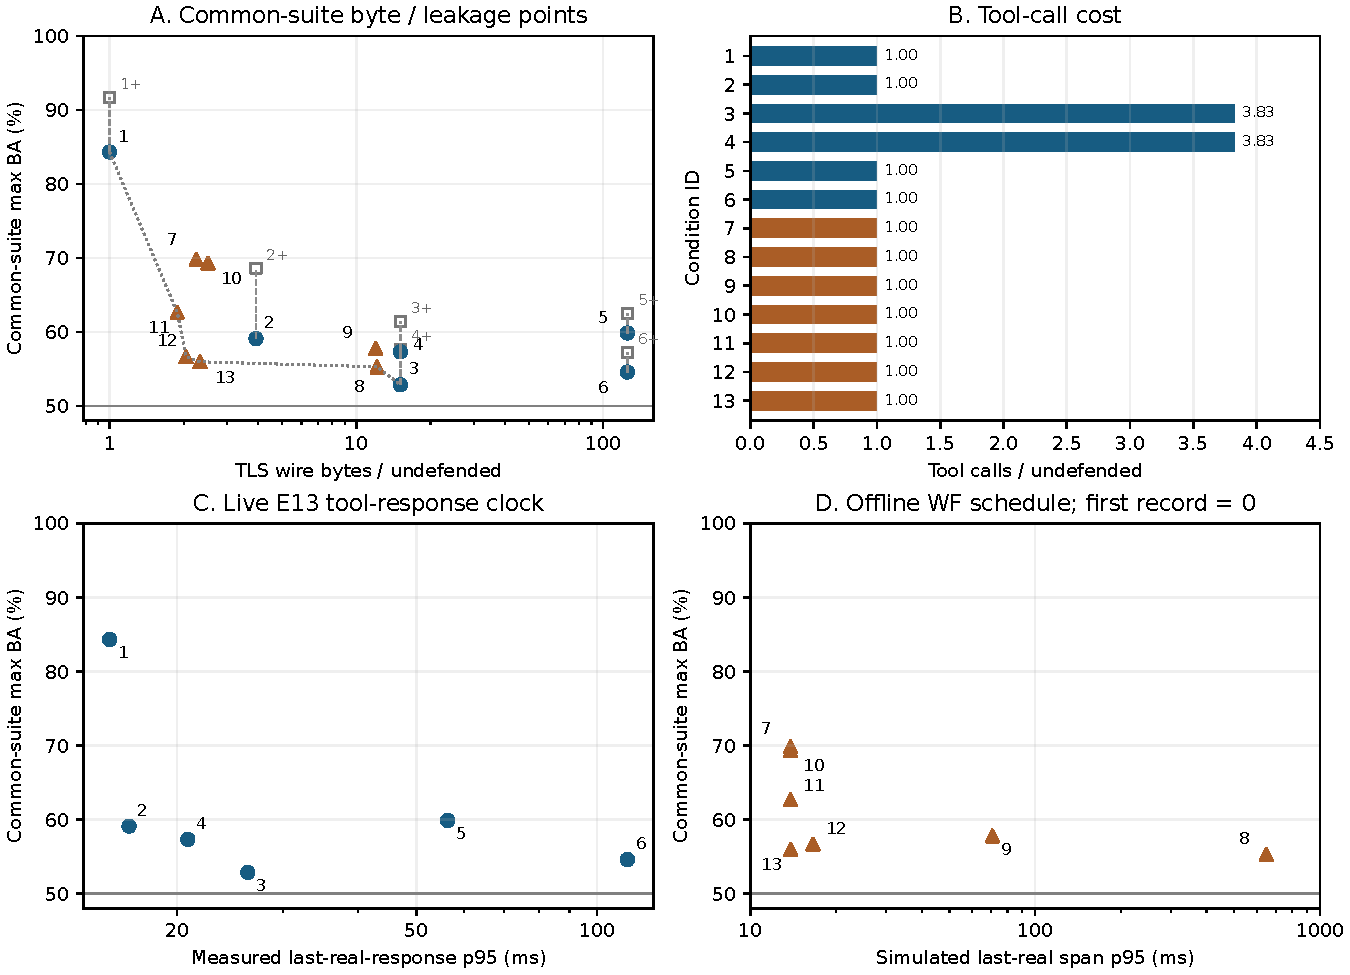
\includegraphics[width=.93\textwidth]{figures/r7-pareto.pdf}
\caption{E14 standard-prompt operating points under the same seven attacks. Labels: 1 undefended, 2 per-call constant, 3 serial shadow, 4 two-in-flight shadow, 5/6 full 2/5\,ms tunnels, 7 record buckets, 8/9 Tamaraw slow/fast, 10 FRONT, 11 WTF-PAD adaptation, 12 random-donor WT, 13 short-calibration FRONT. Gray squares with ``+'' labels in A show larger full-union maxima; dotted nondominance uses only matched colored points and is neither statistically certified nor globally optimal. Circles are measured E13 clocks; triangles are offline transformations. Panels C/D separate time semantics.}
\label{fig:r7-pareto}\end{figure}

Measured delays start at the RPC measurement origin; simulated spans start at the first input record. Zero added delay in FRONT/WTF-PAD's trace transformation does not measure contention on a live link. Actual tool-call ratios remain one for cell-only controls; shadow rows include extra executions. Neither delay panel measures timing-dependent LLM replanning. Thus the byte/BA comparison is shared, while a complete same-scheduler online Pareto comparison remains unperformed.

\subsection{Prospective sample planning}
The planning script varies positive/negative customer counts, assumed BA and attacker dependence using 20,000 binomial trials per setting. It assumes independent customer correctness with equal sensitivity and specificity and a normal 97.5\% upper endpoint, omits the AUROC gate, and is not a power estimate for the observed heterogeneous bootstrap. One attacker also models perfect dependence; seven independent attackers supply a contrasting multiplicity scenario. Under chance-level population BA and three negatives per positive, the searched 80\%-power points are 75 positive customers for one attacker and 150 for seven. Thirty positives is a feasibility floor, not a guaranteed pass. At BA .55, requirements are substantially larger. The planning grid extends the frozen description's 250-customer maximum to 400; this post hoc range extension is recorded in the artifact errata. New independent customer/template sampling must precede a population-level absolute-bound claim.
\begin{table}[ht]\centering\small
\caption{Planning sensitivity: smallest searched positive-cluster count with at least 80\% probability of an upper BA bound below .60. Independent Bernoulli customer correctness and a normal 97.5\% upper endpoint; this omits the AUROC gate and is not the power of the observed heterogeneous bootstrap.}\label{tab:r7-power}
\begin{tabular}{@{}rrrr@{}}\toprule
Negatives per positive & Population BA & Independent attacks & Positive clusters\\\midrule
1 & 0.50 & 1 & 100\\
1 & 0.50 & 7 & 200\\
1 & 0.55 & 1 & 400\\
1 & 0.55 & 7 & $>400$ in grid\\
3 & 0.50 & 1 & 75\\
3 & 0.50 & 7 & 150\\
3 & 0.55 & 1 & 400\\
3 & 0.55 & 7 & $>400$ in grid\\
\bottomrule\end{tabular}\end{table}


The prospective validation file specifies new environment/model versions, precollection customer splits, training-only calibration, the unchanged BA/AUROC gates, live planner utility measurements and blind-human recoding. It is a future protocol, not a completed collection or an external preregistration. Repeated old tasks, a same-provider model extension and AI source review do not satisfy these independent validation requirements.

\clearpage
\section{Expanded Cross-Fitted Attacks and Oracle Localization}\label{sec:r7-crossfit-supp}
This extension reanalyzes the existing 690 Sol episodes with the same five customer folds as E10. It is post hoc: the cohort, defense design and prior results were already available. The new source/configuration freeze precedes the new fits, not the original test collection. All 53 customers are retained, with 14 cancellation-positive and 18 return-positive customers. Each prompt contributes 345 out-of-fold episodes. Fold sizes are 11/12/10/10/10 customers; a rare joint-label stratum has only three customers, so not every fold can contain that stratum. The saved fold assignment and customer/target counts make this restriction explicit.

\subsection{Complete attack union and fitting boundary}
For each fold, joint count templates, cover donors, framing caps and size-to-tool decoders use only the other four folds. The extended union retains all nine prior network attacks: majority, undefended-data-trained gradient boosting, D2 logistic regression and gradient boosting, random forest, nearest neighbors, and three decoded-profile attacks. It adds the fixed trained 1D-CNN and k-FP-style leaf attack described in S20. CNN inputs are direction, log record length and a mask; the timing channel is identically zero because this analysis concerns length/order. No interarrival times are synthesized. The mapping from archived C/S direction strings to numeric signs is explicit and checked. An initial mapping error stopped before any prediction pack was produced; its failed protocol snapshot is retained separately.

All 60 fold/prompt/condition/target packs preserve their fitted learners, test scores and predictions. Out-of-fold rows are pooled only after every fold is evaluated. Each of 2,000 common customer-bootstrap draws retains a customer's tasks and repetitions together and reselects the full 11-attack maximum. Paired decreases use the same draw for undefended and defended conditions. These intervals condition on the fitted attackers and original cohort. The absolute gate remains an upper BA bound below .60 and suite-maximum AUROC below .65. Neither an attack's favorable point estimate nor an increase in the number of resampled trajectories replaces independent positive customers.

\begin{longtable}{@{}lllrrrr@{}}
\caption{Expanded E10: all 12 cells. Percent BA and paired undefended-minus-defended decrease, each with 95\% customer-bootstrap intervals. AUROC is independently maximized over the same 11 attacks. Ratios are bytes/calls.}\label{tab:r7-crossfit-all}\\
\toprule Prompt & Condition & Target & BA [95\% CI] & AUROC & Decrease [95\% CI] & B$\times$/C$\times$\\\midrule\endfirsthead
\toprule Prompt & Condition & Target & BA [95\% CI] & AUROC & Decrease [95\% CI] & B$\times$/C$\times$\\\midrule\endhead
Standard & Undefended & cancel & 91.7 [82.1, 100.0] & 0.979 & -- & 1.00/1.00\\
Standard & Undefended & return & 85.5 [76.7, 93.4] & 0.897 & -- & 1.00/1.00\\
Standard & Joint constant & cancel & 60.5 [52.9, 72.4] & 0.594 & 31.2 [15.3, 41.0] & 19.76/5.04\\
Standard & Joint constant & return & 55.5 [51.8, 64.2] & 0.533 & 30.0 [14.8, 39.2] & 19.76/5.04\\
Standard & Joint buckets & cancel & 57.1 [50.0, 71.5] & 0.579 & 34.6 [15.1, 46.4] & 12.36/5.04\\
Standard & Joint buckets & return & 52.7 [50.0, 61.7] & 0.536 & 32.8 [20.8, 38.9] & 12.36/5.04\\
Rules & Undefended & cancel & 90.7 [81.5, 98.9] & 0.978 & -- & 1.00/1.00\\
Rules & Undefended & return & 85.5 [76.6, 93.6] & 0.880 & -- & 1.00/1.00\\
Rules & Joint constant & cancel & 58.8 [52.1, 71.6] & 0.581 & 32.0 [13.1, 44.2] & 19.88/5.04\\
Rules & Joint constant & return & 59.4 [54.2, 68.8] & 0.581 & 26.1 [11.1, 36.6] & 19.88/5.04\\
Rules & Joint buckets & cancel & 56.9 [50.2, 71.2] & 0.573 & 33.8 [14.2, 45.8] & 12.45/5.04\\
Rules & Joint buckets & return & 52.7 [50.0, 65.0] & 0.565 & 32.8 [19.0, 39.8] & 12.45/5.04\\
\bottomrule\end{longtable}


\subsection{What changes under stronger attacks}
In the standard-prompt arm, the CNN raises bucketed cancellation inference to 57.1\%, and the leaf-fingerprint learner raises constant-framing return inference to 55.5\%. The corresponding paired decreases from undefended transport remain positive: 34.6 points [15.1,46.4] and 30.0 points [14.8,39.2]. This exploratory comparison shows measured reduction with an unresolved absolute bound. It is not tied to the original 50\% frozen-split realization. Both prompt arms and every evaluated operating point are retained, including rules-arm estimates that differ from the standard prompt. The main descriptive table reports the complete union; S15 retains the earlier suite and six-point selection analysis as historical context.

The extension saves 4,140 out-of-fold condition/target rows and checks all 45,540 attack scores against the fitted model archives. Input hashes preserve the original cohort and folds; a documented path map permits read-only verification after checkout relocation without changing frozen source paths or data hashes.

\subsection{Expanded oracle localization}
A separate before-fit extension reuses the original E12 oracle filter and the same five folds. It retains or removes complete exchanges belonging to true state-changing calls, then exposes only network record directions and lengths to attackers. Tool identities choose the diagnostic subset but are not attack features. The full-view reference is the verified expanded E10 undefended output. All nine prior attacks plus the same fixed CNN and forest-leaf learners are fitted for each oracle view, yielding 40 additional fold packs and 2,760 out-of-fold rows. Exact model reloading and legacy refitting check 30,360 scores, customer separation, labels and the full-view reference. Empty filtered traces remain included.

\begin{longtable}{@{}lllrr@{}}
\caption{Expanded E12 oracle ablation, both prompts. Suite-maximum BA (percent) and AUROC, with customer-bootstrap 95\% intervals. The full reference is the verified expanded E10 undefended prediction set.}\label{tab:r7-e12-all}\\
\toprule Prompt & Target & Oracle view & BA [95\% CI] & AUROC [95\% CI]\\\midrule\endfirsthead
\toprule Prompt & Target & Oracle view & BA [95\% CI] & AUROC [95\% CI]\\\midrule\endhead
Standard & cancel & Full trace & 91.7 [82.1, 100.0] & 0.979 [0.949, 1.000]\\
Standard & cancel & Writes removed & 62.8 [54.6, 75.3] & 0.611 [0.533, 0.768]\\
Standard & cancel & Writes only & 91.7 [82.1, 100.0] & 0.973 [0.936, 1.000]\\
Standard & return & Full trace & 85.5 [76.7, 93.4] & 0.897 [0.849, 0.965]\\
Standard & return & Writes removed & 59.9 [52.2, 71.8] & 0.657 [0.571, 0.789]\\
Standard & return & Writes only & 84.9 [78.8, 94.0] & 0.906 [0.864, 0.973]\\
Rules & cancel & Full trace & 90.7 [81.5, 98.9] & 0.978 [0.954, 0.999]\\
Rules & cancel & Writes removed & 68.7 [59.4, 80.2] & 0.690 [0.593, 0.822]\\
Rules & cancel & Writes only & 90.7 [81.4, 98.9] & 0.968 [0.930, 0.998]\\
Rules & return & Full trace & 85.5 [76.6, 93.6] & 0.880 [0.805, 0.955]\\
Rules & return & Writes removed & 66.5 [56.5, 77.7] & 0.664 [0.579, 0.807]\\
Rules & return & Writes only & 85.1 [78.6, 93.7] & 0.917 [0.862, 0.978]\\
\bottomrule\end{longtable}


For the standard prompt, write exchanges constitute 19.6\% of real calls and 23.4\% of TLS wire bytes, yet retain 91.7/84.9\% BA versus 91.7/85.5\% for full traces. Removing writes reduces the suite maximum by 28.9 points [10.7,41.9] for cancellation and 25.6 [11.0,35.4] for returns. The rules-arm decreases are 22.0 [6.0,35.1] and 19.0 [6.0,30.1] points. Read-only traces still carry measurable information; this is concentration of the main signal, not exclusive localization. The small full-minus-writes-only point difference does not constitute a formal equivalence test. Per-prompt read/write retained-call and byte fractions sum to one and are checked against the original trace projection.

\clearpage
\section{Additional Same-Provider Real-Agent Study (E15)}\label{sec:r7-luna}
This supplementary study tests another model alias on actual tool decisions while keeping the original 690 Sol episodes unchanged. GPT-6 Luna with low reasoning effort serves as the planner and, in a separate context, the user simulator. The authenticated subscription interface returns structured actions; the harness executes them in the public retail sandbox and returns the actual observations. Requested and returned model identifiers, instructions, requests, raw events and decisions are archived. Ten pilot episodes are excluded from the 150 formal episodes.

\subsection{Sample, collection and analysis boundaries}
The convenience sample contains 75 existing tasks: the first 29 inherited training tasks after excluding pilot IDs 0--4, plus all 46 inherited test tasks. Each has standard and rules prompts and one repetition. This gives 58 training and 92 test episodes from 10 and 24 nonoverlapping customers. The training customers include two cancellation-positive and seven return-positive customers; the test set includes five and seven. All customers and tasks were available during earlier manuscript development. The collection fingerprint fixes the model alias, effort, instructions, tool schema, code and customer split.

The appended dispatch/network algorithms and configuration were frozen after 44 formal episodes, before any formal test output. Defense parameters were fitted after the complete collection, using only the 58 training episodes; unlike E9, the fitted parameters were not frozen before test collection. Every completed formal episode remains included, irrespective of task reward, unknown tool attempts or protocol errors. Infrastructure failures are distinct from unsuccessful task outcomes. Table~\ref{tab:r7-luna-utility} reports reward, elapsed time and errors. These clocks include model interaction and local execution under the collection service, rather than estimating latency under cover.

\begin{table}[ht]\centering\footnotesize
\caption{Additional Luna study: all 75 runs per prompt, including task failures. Tool counts are dispatches to registered tools, including failed calls; tool errors also include unknown-name attempts. Wall-clock time covers model interaction and local execution. These are undefended planner runs, not live-cover replanning.}\label{tab:r7-luna-utility}
\begin{tabular}{@{}lrrrrrr@{}}\toprule
Prompt & Reward & \shortstack{Median / p95\\(s)} & \shortstack{Tool / model\\calls} & \shortstack{Tool\\errors} & \shortstack{Protocol\\errors} & \shortstack{Infra / timeout\\/ retry}\\\midrule
Standard & 32/75 & 92.5 / 159.0 & 498 / 1530 & 36 & 3 & 0 / 0 / 0\\
Rules & 33/75 & 92.5 / 175.5 & 505 / 1542 & 37 & 4 & 0 / 0 / 0\\
\bottomrule\end{tabular}\end{table}


The standard and rules arms obtain 32/75 and 33/75 native rewards. Median episode time is 92.5\,s in both arms; the respective 95th percentiles are 159.0 and 175.5\,s. There are three and four protocol-error episodes, retained in the analysis. The collection records zero infrastructure errors, timeouts or automatic retries; this does not imply all tasks succeeded. These are descriptive within-study outcomes, not a controlled performance ranking against the differently sampled Sol cohort.

\subsection{Dispatch diagnostic and local TLS replay}
The dispatch diagnostic fits a majority control, logistic regression and gradient boosting to each prompt/view/target on its 29 training episodes. The all, writes-only and reads-only views expose tool names and response lengths. Reads-only retains names beginning with get/find/list; it excludes other non-write calls and is therefore different from the complete writes-removed complement in Sol E12. The archive records all retained/excluded names and counts. The inherited gradient-boosting minimum leaf size is 20: with 29 training rows it cannot split. This fixed model is retained and its constant predictions are disclosed; the suite maximum must be read in light of this small training set. Table~\ref{tab:r7-luna-dispatch} reports all 12 cells.

The network analysis pools only the training episodes to fit count templates, other-customer donor pools and framing caps. Each trajectory is replayed through undefended, per-call padding, shape cover and joint conditions, producing 600 actual TLS~1.2 loopback sessions. Unknown-tool error exchanges are retained; they are dispatch attempts rather than successful simulator-tool executions. The network projection contains directions, lengths and order, excluding provider traffic and arrival timing. The inherited R4 suite includes undefended-trained $D_0$, condition-refitted $D_2$ and training-derived decoder/count controls, evaluated per prompt. It is distinct from the expanded 11-attack Sol cross-fit suite. Table~\ref{tab:r7-luna-network} retains all 16 network cells. Both analyses reselect the suite maximum in each of 2,000 customer-bootstrap draws and exclude draws missing a class. The intervals condition on the fitted predictions.

{\footnotesize
\begin{longtable}{@{}lllrrr@{}}
\caption{Luna dispatch-view diagnostic: maximum over majority, D2 logistic regression and D2 gradient boosting. Each prompt uses 29 training and 46 test tasks. Percent BA and AUROC have customer-bootstrap 95\% intervals. Read-only retains only get/find/list prefixes; it is not Sol E12's entire writes-removed complement.}\label{tab:r7-luna-dispatch}\\
\toprule Prompt & View & Target & BA [95\% CI] & AUROC [95\% CI] & Valid draws\\\midrule\endfirsthead
\toprule Prompt & View & Target & BA [95\% CI] & AUROC [95\% CI] & Valid draws\\\midrule\endhead
Standard & all & cancel & 78.3 [50.0, 96.2] & 0.829 [0.619, 0.959] & 1994/2000\\
Standard & all & return & 63.2 [50.0, 78.4] & 0.691 [0.502, 0.842] & 2000/2000\\
Standard & writes-only & cancel & 87.5 [81.1, 94.6] & 0.925 [0.859, 1.000] & 1994/2000\\
Standard & writes-only & return & 66.6 [53.6, 80.5] & 0.769 [0.582, 0.919] & 2000/2000\\
Standard & reads-only & cancel & 50.0 [50.0, 64.3] & 0.500 [0.500, 0.722] & 1994/2000\\
Standard & reads-only & return & 57.0 [50.0, 74.2] & 0.522 [0.500, 0.758] & 2000/2000\\
Rules & all & cancel & 73.8 [50.0, 98.0] & 0.850 [0.513, 1.000] & 1994/2000\\
Rules & all & return & 67.5 [50.0, 82.2] & 0.782 [0.575, 0.913] & 2000/2000\\
Rules & writes-only & cancel & 89.2 [67.1, 100.0] & 0.917 [0.768, 1.000] & 1994/2000\\
Rules & writes-only & return & 77.8 [60.2, 92.6] & 0.906 [0.769, 0.986] & 2000/2000\\
Rules & reads-only & cancel & 50.8 [50.0, 63.2] & 0.500 [0.500, 0.774] & 1994/2000\\
Rules & reads-only & return & 57.3 [50.0, 75.2] & 0.564 [0.500, 0.800] & 2000/2000\\
\bottomrule\end{longtable}}

{\footnotesize
\begin{longtable}{@{}lllrrrr@{}}
\caption{Luna local TLS replay: all 16 prompt/condition/target cells from 600 sessions. The inherited R4 suite includes undefended-trained $D_0$, condition-refitted $D_2$ and decoder/count controls; it differs from the expanded Sol union. Percent BA and AUROC have customer-bootstrap 95\% intervals. B/C denotes wire-byte and dispatch-record ratios to the same prompt's undefended test replay. Records include unknown/error attempts and generated cover; C is not a successful-action ratio.}\label{tab:r7-luna-network}\\
\toprule Prompt & Condition & Target & BA [95\% CI] & AUROC [95\% CI] & B$\times$/C$\times$ & Gate\\\midrule\endfirsthead
\toprule Prompt & Condition & Target & BA [95\% CI] & AUROC [95\% CI] & B$\times$/C$\times$ & Gate\\\midrule\endhead
Standard & Undefended & cancel & 64.2 [50.0, 100.0] & 0.642 [0.500, 1.000] & 1.00/1.00 & Inconcl.\\
Standard & Padding & cancel & 50.4 [50.0, 69.8] & 0.567 [0.500, 0.781] & 3.98/1.00 & Inconcl.\\
Standard & Shape & cancel & 58.3 [50.0, 70.0] & 0.767 [0.500, 0.955] & 4.25/3.91 & Inconcl.\\
Standard & Joint & cancel & 60.4 [50.0, 72.0] & 0.623 [0.500, 0.724] & 15.57/3.91 & Inconcl.\\
Rules & Undefended & cancel & 65.4 [58.3, 100.0] & 0.667 [0.507, 1.000] & 1.00/1.00 & Inconcl.\\
Rules & Padding & cancel & 57.5 [50.0, 81.1] & 0.542 [0.500, 0.839] & 3.95/1.00 & Inconcl.\\
Rules & Shape & cancel & 55.8 [50.0, 77.4] & 0.579 [0.500, 0.878] & 4.26/3.95 & Inconcl.\\
Rules & Joint & cancel & 59.2 [50.0, 72.5] & 0.569 [0.500, 0.715] & 15.58/3.95 & Inconcl.\\
Standard & Undefended & return & 84.9 [72.2, 100.0] & 0.851 [0.728, 1.000] & 1.00/1.00 & Above\\
Standard & Padding & return & 50.0 [50.0, 56.4] & 0.531 [0.500, 0.702] & 3.98/1.00 & Pass\\
Standard & Shape & return & 54.5 [50.0, 64.3] & 0.500 [0.500, 0.643] & 4.25/3.91 & Inconcl.\\
Standard & Joint & return & 57.0 [50.0, 71.4] & 0.595 [0.500, 0.769] & 15.57/3.91 & Inconcl.\\
Rules & Undefended & return & 90.9 [71.4, 100.0] & 0.909 [0.714, 1.000] & 1.00/1.00 & Above\\
Rules & Padding & return & 50.0 [50.0, 70.9] & 0.500 [0.500, 0.669] & 3.95/1.00 & Inconcl.\\
Rules & Shape & return & 59.1 [50.0, 75.0] & 0.500 [0.500, 0.750] & 4.26/3.95 & Inconcl.\\
Rules & Joint & return & 50.0 [50.0, 57.1] & 0.500 [0.500, 0.617] & 15.58/3.95 & Pass\\
\bottomrule\end{longtable}}


\subsection{Observed model sensitivity}
Writes-only dispatch BA is 87.5/66.6\% for standard and 89.2/77.8\% for rules, compared with reads-only 50.0/57.0\% and 50.8/57.3\%. This reproduces the qualitative write-associated pattern in a smaller dispatch diagnostic. It does not estimate an equivalent Sol/Luna effect because the attack suite, read view, repetition count and cohort differ.

Undefended network BA is 64.2/84.9\% for standard and 65.4/90.9\% for rules. Joint shaping gives 60.4/57.0\% and 59.2/50.0\%, at 15.57/15.58$\times$ wire bytes and 3.91/3.95$\times$ dispatch records. Per-call padding alone gives 50.4/50.0\% and 57.5/50.0\%: joint shaping does not uniformly improve this smaller suite's point estimates. The original gate requires a BA upper 95\% bound below .60 and maximum AUROC below .65. Two of 16 cells meet it (standard padding/return and rules joint/return); none of the conditions meets it for both targets in either prompt arm. The observed constant-score diagnostic covers every fitted gradient booster, including the inherited network and decoder variants, while logistic regression remains nonconstant. These findings motivate population- and attacker-specific calibration rather than a universal ranking of the program conditions.

\subsection{Validation and scope}
The executable audit reconstructs native reward in fresh sandbox states and checks every model answer against the completed raw event, request-history prefix, subsequent assistant/tool record, arguments, response bytes and usage totals. A public raw archive redacts only the local home-directory prefix, retaining per-file original/public hashes. The same decision alignment and reward reconstruction use this public archive and the pinned benchmark/tool sources in the package, without reading the original raw directories. Training-only recalibration, 600 TLS replays and 32 dispatch/network result cells reproduce the saved BA/AUROC estimates and intervals. A separate replay of the 12 dispatch-view cells exactly matches all 36 per-model prediction sets and suite statistics. A derived receipt separates dispatches to known tool names from all dispatch attempts; known-tool counts include failed calls. The original frozen verifier's receipt is retained with an explicit field-label correction. Network call ratios use all test dispatch records, including unknown/error attempts and, in shaped conditions, generated cover exchanges; they do not count successful actions.

This extension adds real model trajectories and a reusable evidence archive. Different cohort sampling, one repetition, the same provider/user simulator, few positive customers and weaker inherited attacks preclude a causal model ranking or an independent replication of Sol E12. Replayed program conditions preserve logical outcomes by construction. The study does not measure live-cover LLM replanning, a second environment, fixed open weights, another provider or new independent customers.


\clearpage
\section{R8 Construct validity and evidence calibration}\label{sec:r8-empirical-audit}
This appendix applies the paper's evidence requirements to its own experiments. It adds deterministic sensitivity calculations on saved predictions, not new model runs, customers or defense deployments. The separate analysis plan and code hashes were frozen before these new calculations; the original test predictions were already available, so this remains post hoc.

\subsection{Customer composition and fixed-attacker sensitivity}
The complete out-of-fold prediction collection contains 690 original model trajectories, re-used across conditions and targets. Each prompt-specific cell contains 345 trajectories (115 tasks, three repetitions), but only 53 customers. Cancellation has 54 positive trajectories from 18 tasks and 14 customers; return has 96 from 32 tasks and 18 customers. These full-cohort positive-customer counts differ from the original held-out subset's five/seven. Repetitions, prompts and transformed views do not create additional independent customers.

For each of the 11 saved attackers, episode-weight BA pools correctness within each true class. The sensitivity estimand first averages correctness within each customer/class stratum, then equally weights customers within each class and finally the two class rates. The four cancellation and eight return mixed-label customers contribute separately to both class rates; they are neither discarded nor forced to have one customer-level label. Suite maxima are independently reselected under both weightings. Thresholds and predictions remain fixed.

\begin{table*}[ht]\centering\footnotesize
\caption{Fixed-prediction cluster sensitivity for the complete OOF cohort. BA and leave-one-positive-customer-out ranges are percentages. Each row has 345 trajectories and 53 customers. Every deletion removes the customer's negative tasks as well as positive tasks; all 14/18 deletions remain valid for cancel/return. Ranges are deterministic influence ranges, not confidence intervals.}\label{tab:r8-cluster-sensitivity}
\begin{tabular}{@{}lllrrrr@{}}\toprule
Prompt & Condition & Target & Episode BA & Customer-equal BA & LOO episode range & LOO customer-equal range\\\midrule
Standard & Undefended & cancel & 91.67 & 94.05 & 90.62--96.67 & 93.59--96.15\\
Standard & Undefended & return & 85.49 & 85.76 & 84.17--87.65 & 84.98--87.96\\
Standard & Joint bucket & cancel & 57.07 & 54.80 & 54.30--61.59 & 53.70--57.55\\
Standard & Joint bucket & return & 52.71 & 56.48 & 51.04--54.72 & 55.11--58.05\\
Standard & Joint constant & cancel & 60.50 & 58.96 & 57.26--61.98 & 56.90--60.74\\
Standard & Joint constant & return & 55.46 & 53.15 & 53.37--56.72 & 51.37--54.27\\
Rules & Undefended & cancel & 90.74 & 92.86 & 89.58--95.56 & 92.31--94.87\\
Rules & Undefended & return & 85.49 & 85.85 & 84.17--87.65 & 85.08--88.06\\
Rules & Joint bucket & cancel & 56.90 & 54.71 & 54.12--61.42 & 53.61--57.45\\
Rules & Joint bucket & return & 52.67 & 53.42 & 51.66--54.22 & 52.44--53.91\\
Rules & Joint constant & cancel & 58.75 & 56.60 & 55.17--60.86 & 54.16--58.12\\
Rules & Joint constant & return & 59.40 & 60.40 & 57.59--62.17 & 59.28--62.23\\
\bottomrule\end{tabular}\end{table*}

Weighting changes the estimand and moves different cells in different directions; it is not a universal correction in favor of either defense. Positive-customer deletion exposes concentration in particular customers. Neither calculation removes that customer's influence on models trained in other folds: no attacker is refitted. Thus these results condition on the saved fitted attacks and do not include retraining uncertainty, an independent population, or uncertainty induced by prior development access to the public tasks. We do not pool scores into one customer-level classifier because task labels can differ within a customer. The complete per-attack, per-customer/class and per-deletion values, including remaining denominators, are saved in \texttt{sp2027-r8-cluster-sensitivity/results.json}; an independent direct-weight verifier checks all 12 cells and 192 deletions.

\subsection{Applying R1--R9 to our own evidence}
Table~\ref{tab:r8-own-evidence} distinguishes a bound measurement from an unverified extension. In particular, a structural planner-history invariant, measured fixed-action response/state equality, and live LLM task utility are different outcomes. Inherited native reward does not count as utility measured under the defended operating point.

\begin{table*}[ht]\centering\footnotesize
\caption{Scoped self-audit of E9/E10/E13/E14/E15 under R1--R9. Entries describe evidence boundaries, not overall success grades. The missing live defended-LLM utility binding is retained for our experiments under the same standard applied to the source corpus.}\label{tab:r8-own-evidence}
\begin{tabularx}{\textwidth}{@{}lYY@{}}\toprule
Item & Bound or partially bound observation & Unverified extension\\\midrule
R1: target/polarity & Privacy inference of cancel/return action-labelled task trajectories & Unobserved psychological intent or a general semantic secret\\
R2: receiver & E9/E10/E15 dispatch or TLS length/order; E13 local arrival timing & Production provider logs, routing leaks and unmeasured observers\\
R3: placement/execution & E13 executes tools on fixed saved actions; E14 separates measured and offline rows & Live LLM replanning under cover; executing WF transforms as production defenses\\
R4: defended fitting & Training-only calibration and condition-specific attack fitting; E15 fits only 58 training trajectories & Arbitrary attacker strength or prospective parameter freeze for E15\\
R5: matched adaptation & Defended-data attackers; common-seven condition comparison in E14 & A fully matched clean-versus-adapted causal contrast from every D2/union difference\\
R6: workload shifts & Customer splits/cross-fitting, two prompts and same-provider Luna retail alias & New customers, new environment, independent vendor or blinded confirmation\\
R7: inference & Saved suite maxima, customer intervals, failures and negative outcomes retained & An absolute bound against unknown attackers or success inferred from a low point estimate\\
R8: utility & Original LLM rewards; E13 measured real-response/final-state equality on fixed actions & Live defended LLM task utility; timing-dependent replanning, quotas and failures\\
R9: cost & E13 local tool-chain cost; E14 matched byte/call accounting with separate simulated clocks & End-to-end deployed cost or a common live latency ranking across measured/simulated rows\\
\bottomrule\end{tabularx}\end{table*}

E9/E10 program conditions inherit reward from reused trajectories. E13 additionally checks real responses and final live database states in all 4,140 local sessions, but the next action is specified by the saved trajectory rather than a new LLM decision. E14's offline WF adapters preserve abstract fragment identity/order and do not schedule fragments before input availability; they neither decrypt and compare payloads nor execute tools. Their copied native rewards are not independent utility measurements. E15's actual 150-task rewards and wall clocks describe the original collection service, not planner behavior under cover. Own live defended-LLM utility therefore remains unbound.

\subsection{Matched-seven comparison and the limits of dominance}
All rows in Table~\ref{tab:r8-matched-seven} use the same seven attack families: majority, logistic, gradient boosting, random forest, extra trees, leaf fingerprint and sequence CNN. BA and AUROC suite maxima are separately reselected in each customer-bootstrap draw. The measured conditions retain additional E13 attacks in the full-union assessment elsewhere; this common subset cannot replace that stronger assessment. The exact values, intervals, full-union values and cost denominators are retained in \texttt{provenance/r8-review/defense-self-audit.json}.

\begin{table*}[ht]\centering\footnotesize
\caption{Both prompts under the matched seven-model subset. BA is cancel/return in percent. Bytes and dispatch counts use the corresponding prompt's undefended totals; per-prompt evaluation has 138 trajectories and 24 customers. WT is the random-training-donor RPC adaptation, not the original symmetric-pair guarantee. No row establishes live defended-LLM utility.}\label{tab:r8-matched-seven}
\begin{tabular}{@{}llrrrr@{}}\toprule
Prompt & Condition & Cancel/return BA & Bytes$\times$ & Calls$\times$ & Execution\\\midrule
Standard & WT random donor & 50.00/56.67 & 2.040 & 1.000 & Offline\\
Standard & Serial shadow & 50.00/52.86 & 15.106 & 3.827 & Local tools\\
Standard & Two-in-flight shadow & 50.00/57.32 & 15.106 & 3.827 & Local tools\\
Standard & Full tunnel 2 ms & 59.86/55.19 & 125.706 & 1.000 & Local tools\\
Standard & Full tunnel 5 ms & 54.58/53.68 & 125.706 & 1.000 & Local tools\\
Rules & WT random donor & 51.39/56.28 & 2.233 & 1.000 & Offline\\
Rules & Serial shadow & 56.11/59.78 & 15.468 & 3.882 & Local tools\\
Rules & Two-in-flight shadow & 56.94/57.06 & 15.468 & 3.882 & Local tools\\
Rules & Full tunnel 2 ms & 52.78/55.28 & 128.384 & 1.000 & Local tools\\
Rules & Full tunnel 5 ms & 58.33/54.33 & 128.384 & 1.000 & Local tools\\
\bottomrule\end{tabular}\end{table*}

WT's lower byte and backend-call cost is a real advantage of the evaluated adaptation. For standard prompts it exchanges lower cost for higher return BA than serial shadow (56.67\% versus 52.86\%); neither point dominates the other. For rules, WT has lower point BA on both targets and lower byte/call cost than either shadow scheduler. It also weakly dominates the standard two-in-flight point in these four dimensions. These are descriptive point relations, not statistically certified or deployment dominance: they exclude AUROC and latency, intervals are wide, and the WT schedule is simulated while the shadow tool chain is measured. A claim including AUROC can change the ordering. Tunneled dummies execute no tools; the two fixed local tunnel operating points trade much larger byte cost for no extra backend calls, without establishing an optimal tunnel configuration. The evaluated shadow policy is therefore not presented as Pareto-superior to these controls.

\paragraph{What flush recognition establishes.}
The E13 serial/parallel flush detectors achieve 90.45/92.31\% BA on 15,278 record labels (8,902 after the declared flush start, 6,376 before), pooling 276 trajectories and 24 customers across prompts. This is schedule-phase recognition, not intent recovery. Separate real/cover request detection reaches 82.53/96.08\% BA on 7,639 requests. These observations refute cover-indistinguishability for the measured scheduler/view. Already-saved attacks estimate a single flush boundary using a training-fitted detector, with customer-out-of-fold segmentation for intent training, then attack the remaining prefix. The highest such intent BA is 60.69\% (rules serial return, 95\% interval [50.83,70.95]); the unstripped views remain in the complete suite. Recognizable flush does not imply 90\% intent recovery, and the relatively low stripped-view points do not erase the stronger unstripped attacks or certify defense success.


\subsection{Scoped reuse audit: applicability and denominators}\label{sec:r8-sok-audit}

\subsection{What the nine items mean}
R1--R9 are checks on whether an observation can be reused for a specified comparison. They are not a quality score for a paper, a safety grade, or a judgment that an original study ought to have performed every possible experiment. Bound means that at least one result record in a family supplies the requested binding; Partial retains both supported and unbound parts; NR-R means the inspected source scope does not report the requested item; NR-V means the source/run/version binding could not be verified; NA means the requested inference is outside the scoped claim. The 20-family matrix is a family-level summary, while result-level records remain distinct where mechanisms or test populations differ.

R4 concerns fitting/calibrating an attacker on protected data when adaptation is part of the reuse question. R5 concerns a matched clean/adapted contrast on the same defended test. Thus R5 does not demand a learned-attacker refit for fixed-rate analytical costs, deterministic namespace controls, or non-learning mechanism benchmarks. Applicability is explicit in the matrix: each item has 11 applicable families for R4 and R5. For R4 the distribution is 4 Bound, 1 Partial, 1 NR-R, 5 NR-V, 9 NA; for R5 it is 2 Bound, 2 Partial, 1 NR-R, 6 NR-V, 9 NA. NR-R and NR-V cells identify missing reporting or binding evidence, not failed experiments.

\begin{table*}[t]\centering\footnotesize
\caption{R4, R5 and R8 family dispositions. Reasons are scoped to the item, not judgments of overall study quality.}\label{tab:r8-family-reasons}
\begin{tabularx}{\textwidth}{@{}lcccX@{}}\toprule
Family & R4 & R5 & R8 & Scope note\\\midrule
UI Traces & B & B & U & Offline attribution does not report objective task utility.\\
WRA & -- & -- & P & Proxy visibility and executable-decoy utility are not fully joined.\\
NetEcho & B & P & U & Topic prediction is not downstream task utility.\\
Early Bird & B & P & U & Semantic-cache timing is not end-to-end task utility.\\
Whisper Leak & ? & ? & U & Post-defense fit/test binding is unverified; replay volume is not task utility.\\
SpliceLeak & -- & -- & U & QCP component cost; no task-utility outcome.\\
Time Will Tell & ? & ? & U & Threshold fit/test binding unverified; analytical padding cost is not task utility.\\
I Know What You Said & -- & -- & -- & Zero-copy component control; family-level utility item inapplicable.\\
Speculative decoding & ? & ? & -- & Learned attack present; protected fit and matched test unverified; payload is cost, not utility.\\
Dangol workflow & B & B & U & Matched result is capture-scoped; objective workflow utility is unreported.\\
Cloud traffic benchmark & ? & ? & P & Classifier under reformulation; semantic preservation is asserted, not task-tested.\\
Remote timing & -- & -- & U & Fixed-rate analysis does not bind task utility.\\
TDXRay & -- & -- & B & Vocabulary coverage is component utility, not deployment-task utility.\\
SafeKV & -- & -- & U & Detection and serving performance use separate conditions.\\
AHB/Turing & P & ? & B & Online task accuracy is bound; publication-run fit/test binding remains unverified.\\
KV-Gov & -- & -- & U & Simulation, hardware gap and HMAC costs are distinct outcomes.\\
CachePrune & -- & -- & B & QA/summarization outcomes bind selective cache sharing.\\
OTRO & -- & -- & -- & Mechanism microbenchmark has no scoped task-utility outcome.\\
SparLeak & ? & ? & B & \S7.5/Table~4 pairs reconstruction ASR and local ROUGE by model/intensity.\\
Shape and Substance & U & U & U & Inspected scope reports analytic padding, not protected-fit/matched-test or task utility.\\\bottomrule
\end{tabularx}\end{table*}
\noindent\footnotesize B=Bound, P=Partial, U=NR-R, ?=NR-V, --=NA.

For R5, the matrix's applicable denominator is 11, with 2 Bound (2/11), 2 Partial, 1 NR-R and 6 NR-V. Under the narrower interpretation that only explicitly learned/calibrated adaptive-attack experiments call for this matched contrast, Shape and Substance may be recoded NA: 2/10, with 2 Partial and 6 NR-V among the remaining applicable entries. This is a denominator sensitivity, not a correction to the matrix. For R8, the broad item is task \emph{or} component utility: 4 Bound, 2 Partial, 11 NR-R, 3 NA (4/17 applicable). If the estimand is restricted to deployment-task utility, TDXRay's vocabulary-coverage/lookup result is out of scope, yielding 3 Bound, 2 Partial, 11 NR-R and 4 NA (3/16). This alternative does not convert NR-R into an experimental failure. CachePrune's joint R7--R9 binding remains a scoped positive example, not evidence of adaptive robustness.

Across the 20 audited families, the R1--R9 column distributions (Bound/Partial/NR-R/NR-V/NA) are: R1 20/0/0/0/0; R2 17/3/0/0/0; R3 17/3/0/0/0; R4 4/1/1/5/9; R5 2/2/1/6/9; R6 18/2/0/0/0; R7 17/1/2/0/0; R8 4/2/11/0/3; R9 11/3/5/0/1. Each column sums to 20. Machine-readable family mapping and rationale are in \path{provenance/r19-evidence-closure/family-status-overlay.json}; the earlier overlay remains archived.

\subsection{Same-operation semantic-attribute diagnostic (E16)}\label{sec:r8-attribute}
This exploratory analysis addresses a different target from cancel/return. We fix the observed operation to \texttt{return\_delivered\_order\_items}, requesting exactly one item, and predict whether the selected initial-order product belongs to a frozen 15-name digital-device grouping. The benchmark supplies product names, not this broader taxonomy; the grouping is researcher-defined and is not validated as a real-world secret. It was fixed before fitting or inspecting traffic/target associations. The original 690-episode population was already available, so this is not a fresh confirmatory dataset.

\paragraph{Source, alignment and grouping}
The 138 eligible calls occur in 114 episodes. Full-session reconstruction exactly matches the saved raw TLS socket records, including episode hashes, ordered calls and UTF-8 body lengths. We select exact per-call request/response record slices using known call boundaries. This is an oracle diagnostic; it does not demonstrate passive discovery of a call's location. Each feature vector contains record count, total, maximum and minimum length in each direction. No plaintext, identifiers or measured timing are used.

Repeated calls are averaged within prompt/customer/order/item. Each prompt then has 20 instances (9 positive, 11 negative), spanning 15 customers (8 with positives, 9 with negatives, 2 with both). The same 20 instances and aggregated features occur in both prompt arms; the two arms are not independent replications. We retain the original five customer folds. All training folds have both classes; one test fold lacks positives, so results pool OOF predictions rather than average fold BA.

\paragraph{Frozen fits and negative controls}
The pre-fit protocol binds code, input and source hashes. Learners are LR ($C=1$, balanced), RF (200 trees, depth 3, minimum leaf 2), and GB (50 stages, depth 1, learning rate 0.05), with no post-result tuning or orientation reversal. Operation-only and canonical constant-size inputs contain no varying information; a constant-class predictor gives exactly 50\% BA. The order-item-count-only diagnostic retains a potential whole-order-size confounder. A fixed-seed label shuffle within the old folds is shared across repeats/prompts; it is one sanity check, not a permutation distribution or a significance test.

\begin{table}[ht]\centering\footnotesize
\caption{Same-operation attribute diagnostic. Both prompts have identical features and results. Fixed three-model suite maximum BA and 95\% customer-bootstrap interval; 20 instances, 15 customers per prompt.}\label{tab:r8-attribute}
\begin{tabular}{@{}lrr@{}}\toprule
Observation / target & BA (\%) & 95\% interval\\\midrule
Raw record summaries, original target & 30.3 & [16.7,52.7]\\
Constant-class reference & 50.0 & [50.0,50.0]\\
Whole-order item count only & 51.5 & [40.6,68.8]\\
Raw summaries, fixed shuffled target & 65.2 & [47.4,85.7]\\\bottomrule
\end{tabular}\end{table}

The raw fixed-suite maximum is 30.3\%; the original-direction AUROCs are 0.182/0.182/0.187 for LR/RF/GB. These below-chance scores do not imply no information: reverse associations may exist. We preserve the frozen orientation instead of selecting a more favorable attack after seeing the result. The high shuffled-label point further illustrates the instability of this tiny grouped cohort. These results neither establish a stable non-action-attribute attack nor prove absence of such leakage, and provide no evidence of defense effectiveness.

\paragraph{Residual confounding and reproducibility}
Initial whole-order sizes 1/2/3/4/5 have 6/3/2/7/2 instances, with 3/0/1/5/0 positive labels. Fixing the requested count does not balance full-order size. No post-result matching is fitted. Intervals use 2,000 fixed-prediction customer bootstrap draws, omitting one-class draws and recording their count; they exclude refitting uncertainty and target-choice uncertainty. An independent verifier checks the source chain, grouping and repeat aggregation, reloads 150 saved models, reproduces 600 OOF scores and all BA intervals, and verifies positive-class score orientation. Full per-model BA/AUROC, every fold's scores, controls and support counts are retained in the attribute module. Protocol SHA-256: \texttt{c2c7c67363f80a89c5df947380e7f071619}\\\texttt{6844ce4365a2b9770fd732d28ad59}.

\clearpage\section{Additional Endpoint Model Replications}\label{sec:endpoint-replication}

Two endpoint replications each execute 115 tasks once with the standard prompt, using the original 69/46 task and 29/24 customer split. All training trajectories precede defense calibration and test collection. Network interventions replay the same real model trajectories over local TLS; they do not measure defended online replanning. Model aliases are not immutable weight revisions. The deployment owner identifies MiniMax-M3 as a DeepSeek backend; this attribution is not independently verified.

MiniMax uses a 4,096-token output limit. GLM uses 16,384 after an interface preflight exposed truncation; all earlier-interface episodes, including successes, are archived and excluded. GLM requests disable parallel tool calls to match the single-action harness. Transport timeouts resume cached decisions and preserve failed attempts; model protocol failures remain terminal outcomes. The GLM transport waiting limit changed from 180 to 600 seconds without changing inference requests. This budget asymmetry permits within-model defense contrasts, not an equal-budget model ranking.

\subsection{MiniMax-M3}

Native task success is 68/115, including 23 terminal protocol failures in the denominator. The archived verifier passes 5627 checks. These archived endpoint rows use the original six attacks; the subsequent transfer section adds total exchange count and supplies the expanded-suite figures used in the main text. Network BA intervals use 2,000 customer bootstrap draws, reselecting the suite maximum conditional on fitted attackers. The small positive customer counts remain five/seven for cancellation/return.

\begin{center}\begin{tabular}{llll}\toprule

View / condition & Target & BA (\%) & 95\% interval\\\midrule

raw & cancel & 58.3 & [50.0, 83.3]\\

shape\_const & cancel & 60.4 & [50.0, 74.1]\\

raw & return & 83.5 & [68.2, 98.7]\\

shape\_const & return & 59.9 & [50.0, 79.7]\\

all & cancel & 58.3 & [50.0, 83.3]\\

all & return & 83.5 & [68.2, 98.7]\\

writes-only & cancel & 58.3 & [50.0, 80.0]\\

writes-only & return & 83.8 & [72.5, 95.8]\\

writes-removed & cancel & 52.9 & [50.0, 70.5]\\

writes-removed & return & 58.7 & [50.0, 81.4]\\

\bottomrule\end{tabular}\end{center}

\subsection{GLM-5.3-flash}

Native task success is 83/115, including 16 terminal protocol failures in the denominator. The archived verifier passes 5023 checks. These archived endpoint rows use the original six attacks; the subsequent transfer section adds total exchange count and supplies the expanded-suite figures used in the main text. Network BA intervals use 2,000 customer bootstrap draws, reselecting the suite maximum conditional on fitted attackers. The small positive customer counts remain five/seven for cancellation/return.

\begin{center}\begin{tabular}{llll}\toprule

View / condition & Target & BA (\%) & 95\% interval\\\midrule

raw & cancel & 100.0 & [100.0, 100.0]\\

shape\_const & cancel & 50.0 & [50.0, 79.1]\\

raw & return & 86.6 & [73.7, 97.4]\\

shape\_const & return & 67.3 & [58.7, 89.5]\\

all & cancel & 100.0 & [100.0, 100.0]\\

all & return & 86.6 & [73.7, 97.4]\\

writes-only & cancel & 100.0 & [100.0, 100.0]\\

writes-only & return & 78.1 & [67.5, 92.4]\\

writes-removed & cancel & 65.0 & [50.0, 89.5]\\

writes-removed & return & 63.0 & [50.0, 84.6]\\

\bottomrule\end{tabular}\end{center}

\paragraph{Interpretation} Both endpoints reproduce a return-operation signature and its reduction under joint shaping. MiniMax cancellation is weak before defense and does not improve; GLM return retains substantial residual inference. No endpoint establishes the joint absolute screening criterion for both targets. The result strengthens the evidence-binding contribution: protection claims require the model, target, receiver view and calibration population to be specified together. Write-selected TLS captures are oracle localization diagnostics; attackers receive only lengths, directions and order.

\clearpage\section{Attacker and Calibration Transfer Boundaries}\label{sec:transfer-matrices}

This exploratory extension retains the earlier small-suite results and adds the complete inherited endpoint suite plus an exchange-count rule: majority, clean-trained gradient boosting, defended-data logistic regression and gradient boosting, decoded-tool gradient boosting, decoded target-call count, and total exchange count. It is not the larger Sol timing/CNN suite. All thresholds and decoders fit training customers only. Each of 2,000 customer bootstrap draws reselects the maximum; single-class draws are excluded. Point metrics are independently recomputed from saved predictions. Model endpoints share the original task/customer partition; neither has a verified immutable weight revision.

\subsection{Attacker transfer}

Rows train on the source model and test on held-out customers under the target model. Joint conditions retain target-local calibration, so this table isolates attacker transfer. Calibration transfer is a separate experiment below.

\begin{center}\small\begin{tabular}{llllrrl}\toprule

Source & Target & Condition & Target label & BA (\%) & Bytes$\times$ & 95\% interval\\\midrule

MiniMax & MiniMax & Raw & cancel & 58.3 & -- & [50.0, 83.3]\\

MiniMax & MiniMax & Raw & return & 83.5 & -- & [68.4, 98.7]\\

MiniMax & MiniMax & Joint & cancel & 60.4 & -- & [50.0, 74.1]\\

MiniMax & MiniMax & Joint & return & 67.5 & -- & [57.7, 87.2]\\

MiniMax & GLM & Raw & cancel & 75.0 & -- & [59.7, 100.0]\\

MiniMax & GLM & Raw & return & 77.5 & -- & [66.0, 97.4]\\

MiniMax & GLM & Joint & cancel & 50.0 & -- & [50.0, 50.0]\\

MiniMax & GLM & Joint & return & 55.8 & -- & [50.0, 81.1]\\

GLM & MiniMax & Raw & cancel & 65.4 & -- & [54.7, 85.2]\\

GLM & MiniMax & Raw & return & 88.1 & -- & [76.5, 98.7]\\

GLM & MiniMax & Joint & cancel & 67.1 & -- & [50.0, 87.0]\\

GLM & MiniMax & Joint & return & 53.5 & -- & [50.0, 70.0]\\

GLM & GLM & Raw & cancel & 100.0 & -- & [100.0, 100.0]\\

GLM & GLM & Raw & return & 86.6 & -- & [73.7, 97.4]\\

GLM & GLM & Joint & cancel & 50.0 & -- & [50.0, 80.8]\\

GLM & GLM & Joint & return & 67.3 & -- & [58.7, 89.5]\\

\bottomrule\end{tabular}\end{center}

\subsection{Calibration transfer and localized padding}

Source training templates, donors and caps are applied to target trajectories, including target training trajectories used to refit attackers. All 690 sessions are actual local TLS captures. Write-only padding uses true tool identity at the trusted defense boundary; the adversary receives lengths and directions only. It introduces no cover calls. Byte ratios divide summed test wire bytes by target-model undefended test bytes. Test-call ratios (MiniMax/GLM) are 3.36/4.24$\times$ for local joint, 3.11/4.66$\times$ for imported joint and 1.00/1.00$\times$ for write padding. Raw totals are 510/332 calls; request-record counts agree with saved call arrays.

\begin{center}\small\begin{tabular}{llllrrl}\toprule

Source & Target & Condition & Target label & BA (\%) & Bytes$\times$ & 95\% interval\\\midrule

MiniMax & MiniMax & Joint & cancel & 60.4 & 20.06 & [50.0, 74.1]\\

MiniMax & MiniMax & Joint & return & 67.5 & 20.06 & [57.7, 87.2]\\

MiniMax & MiniMax & Write padding & cancel & 50.0 & 1.45 & [50.0, 62.4]\\

MiniMax & MiniMax & Write padding & return & 61.3 & 1.45 & [52.6, 80.2]\\

MiniMax & GLM & Joint & cancel & 70.8 & 18.65 & [60.5, 90.2]\\

MiniMax & GLM & Joint & return & 50.0 & 18.65 & [50.0, 59.2]\\

GLM & MiniMax & Joint & cancel & 50.8 & 17.48 & [50.0, 69.2]\\

GLM & MiniMax & Joint & return & 63.0 & 17.48 & [50.0, 82.9]\\

GLM & GLM & Joint & cancel & 50.0 & 15.95 & [50.0, 80.8]\\

GLM & GLM & Joint & return & 67.3 & 15.95 & [58.7, 89.5]\\

GLM & GLM & Write padding & cancel & 60.0 & 1.51 & [50.0, 87.0]\\

GLM & GLM & Write padding & return & 61.6 & 1.51 & [53.4, 83.1]\\

\bottomrule\end{tabular}\end{center}

\paragraph{Scope of the conclusion} Target-specific contrasts retain the original engineering screen. Expanded-suite MiniMax joint return BA is 67.5\%, versus 59.9\% previously: the added exchange-count attack changes the evaluation contract, not the trajectories. Write-padding comparisons likewise use the expanded-suite 61.3/61.6\% return values.

\paragraph{Paired transfer uncertainty}
Paired contrasts use the same customer draws and reselect each condition's suite maximum. Moving MiniMax calibration to GLM changes cancellation by $+20.8$ points (95\% interval $[-12.6,35.3]$) and return by $-17.3$ points ($[-38.2,-5.3]$). Moving GLM calibration to MiniMax changes cancellation by $-9.6$ ($[-21.1,6.4]$) and return by $-4.5$ ($[-25.0,12.3]$). These conditional intervals distinguish the observed direction of transfer from the precision available for each target; they include no attacker-retraining uncertainty. All eight calibration/write-padding contrasts are saved in the artifact.

\paragraph{Request-field mechanism check}
Exact serialization accounting identifies which request fields contribute variable length. Across 39 MiniMax and 40 GLM return calls, the item-list field contributes 28--70 bytes (means 40.2 and 37.8), whereas the order identifier contributes 25 bytes and payment-method field 39--44 bytes. This explains a source of length variability without identifying a semantic privacy attribute: the accounting omits fields only for diagnosis, not as a valid API intervention. Response size, call count and timing provide additional channels. The earlier same-operation product-category diagnostic remains inconclusive; operation localization cannot be promoted to attribute inference.

\clearpage\section{Live Planner Utility with Prefix Shadow Execution}\label{sec:live-planner-utility}
This exploratory paired study selects 50 existing task IDs by a frozen SHA-based ordering before new collection, with two fresh GLM planner episodes per task. Both agent and user contexts issue new model requests; cached decisions are used only to resume the same episode after transport failure. The 100 episodes use the served GLM alias, native single-tool actions, a 16,384-token budget and ten workers. They share known tasks with earlier studies and are not a new-customer confirmation. Arm order alternates by task parity.

\paragraph{Execution and deadline contract}
The baseline executes real actions in the retail environment. The prefix-shadow arm additionally executes at most one training-template deficit call on isolated state after each real call; its response is hidden from the planner. Both arms delay each real response by 20\,ms, with another 20\,ms for cover. For task IDs divisible by five, the first tool response receives another 200\,ms delay. The 120\,ms deadline is evaluated against this configured delay, not OS scheduling noise. The real operation can already have executed when its response is replaced by a timeout warning; the next planner request sees that warning and can inspect or retry the state. This tests reaction to a controlled execution/observation mismatch. There is no terminal flush, constant TLS framing or actual WAN path in this utility diagnostic.

\begin{center}\small\begin{tabular}{lrr}\toprule
Outcome & Baseline & Prefix shadow\\\midrule
Episodes & 50 & 50\\
Native successes & 37 & 33\\
Terminal protocol failures & 11 & 7\\
Real tool calls & 360 & 390\\
Isolated cover calls & 0 & 390\\
Injected response timeouts & 12 & 12\\
Tool actions following timeout & 96 & 93\\
Final-pass response-wait p95 (ms) & 32.0 & 47.0\\
\bottomrule\end{tabular}\end{center}

\paragraph{Interpretation and verification}
The paired native-success difference is -8.0 percentage points, with a 2,000-draw customer-bootstrap interval [-23.9,6.5] over 37 customers. All protocol failures remain in the denominator. Subsequent actions demonstrate live reactions to timeout observations; their count alone does not establish correct recovery. The verifier rebuilds actual and reference tool states, checks output requirements and native rewards, matches model-request counts, and checks all live-metric rows. Recorded response waits are from the final execution pass: cache recovery deterministically replays completed action prefixes and their delays. The frozen Windows monotonic clock has 15.625\,ms resolution, so sub-tick differences are not resolved. These waits exclude LLM generation and WAN transit, and are not original uninterrupted end-to-end latencies. Reward is measured on the actual model decisions, rather than inherited from an undefended trajectory.

\paragraph{Transport recovery provenance}
An import-order bug selected the shared endpoint adapter, which honored a 180\,s caller timeout despite the live protocol's intended 600\,s transport wait. After 97 completed episodes, explicit adapter resolution selected the local 600\,s implementation; request bodies, model settings, parsing and all cached decisions remained unchanged. The amendment preserves the old adapter, hashes, logs and no-progress stop, and permits bounded recovery after the identified code fix. This infrastructure wait is separate from the experimentally injected 120\,ms tool-response deadline. Failed model outputs are terminal outcomes, not transport retries. The utility estimate applies to this prefix scheduler and fault model; it cannot supply a reward value for the full joint framing/flush replay rows in Exp~3.

\clearpage\section{Complete Record-Mode Synthesis}\label{app:record-modes}
Every record is classified once by its primary measurement mode. Executed collection/prototype includes separately collected conditions and does not imply paired full-workflow utility. A simulated or derived result remains in that category even when its parameters were measured. Two placement-unresolved records remain explicit. This exhaustive census supplies the denominator for the three explanatory lenses in the main paper; those lenses are retrospective illustrations, not a prevalence sample.
\begin{longtable}{@{}p{.30\textwidth}p{.25\textwidth}p{.38\textwidth}@{}}\toprule Record & Mode & Source locator\\\midrule\endhead
UI-delay-offline~\cite{uitraces2026} & Trace transformation & 6.1 Fig5;A.5\\
WRA-decoy-execution~\cite{jeong2026wra} & Executed collection or prototype & 8.1-8.3 Tables8-11\\
NET-upstream-local~\cite{netecho2025} & Executed collection or prototype & IV-C-E TableIII-IV\\
NET-dummy-padding-simulation~\cite{netecho2025} & Trace transformation & VII TableIX\\
EARLY-K-calibration-oracle~\cite{earlybird2025} & Simulation or derived estimate & V-A TableVI;IV-A\\
EARLY-semantic-deidentification~\cite{earlybird2025} & Executed collection or prototype & V-B\\
WHISPER-randompadding-capture~\cite{whisperleak2025} & Executed collection or prototype & 6.1 Tables3-4\\
WHISPER-batching-replay~\cite{whisperleak2025} & Trace transformation & 6.2 Fig7\\
WHISPER-injection-replay~\cite{whisperleak2025} & Trace transformation & 6.3 Table5\\
SPLICE-CTBF-signal~\cite{spliceleak2026} & Executed collection or prototype & VII-C TableII\\
SPLICE-QCP-cost~\cite{spliceleak2026} & Component or calibration measurement & VII-C TableII\\
TIME-length-instruction~\cite{timewilltell2024} & Executed collection or prototype & 7.2\\
TIME-padding-estimate~\cite{timewilltell2024} & Simulation or derived estimate & 7.3\\
SPEC-padding-REST~\cite{wei2024speculation} & Placement unresolved & 6.1 Fig6-7 Table2\\
DANGOL-capture~\cite{dangol2026workflow} & Trace transformation & 9.8-9.9 Table6\\
DANGOL-livebinding~\cite{dangol2026workflow} & Executed collection or prototype & 9.7, OHTTP paragraph after Table 5\\
SIG-common-guardrail~\cite{geng2026sigleak} & Executed collection or prototype & 4.1-4.2;AppendixC\\
SAFE-post-trigger~\cite{chu2025safekv} & Executed collection or prototype & 7.2.4 Fig12;7.3-7.4\\
AHB-online-executed~\cite{zhu2026turing} & Executed collection or prototype & 5.1.2 Table1;E.1-E.3\\
AHB-offline~\cite{zhu2026turing} & Trace transformation & Table1 offline rows;E.1-E.3\\
KVGOV-partialflush-sim~\cite{addagada2026kvgov} & Simulation or derived estimate & 5.1-5.3\\
KVGOV-hardware-gap~\cite{addagada2026kvgov} & Component or calibration measurement & 5.7-5.8\\
KVGOV-HMAC-cost~\cite{addagada2026kvgov} & Component or calibration measurement & 5.9\\
TRAFFIC-prompt-reformulation~\cite{pouryousef2026traffic} & Executed collection or prototype & V-C1 Fig9a\\
TRAFFIC-temperature~\cite{pouryousef2026traffic} & Executed collection or prototype & V-C1 Fig9a\\
CARLINI-fixed-rate~\cite{carlini2024remote} & Placement unresolved & VII Fig11-12\\
GAO-zero-copy-off~\cite{gao2025iknow} & Component or calibration measurement & 7.1\\
TDXRAY-oblivious-map~\cite{hornetz2026tdxray} & Component or calibration measurement & 6.1 Fig8 Table3\\
AGENTTELL-fixed-instruction~\cite{shahriar2026agenttell} & Executed collection or prototype & 4.3.1;5 Finding1\\
FP-CLOUDFLARE~\cite{wang2026fpagent} & Executed collection or prototype & 6.4 Table5\\
BAR-co-running-noise~\cite{gu2026behindbars} & Executed collection or prototype & 7.2-7.3 Table8\\
RHYTHM-VPN~\cite{alhazbi2025rhythm} & Executed collection or prototype & VI-B;VII\\
DEB-filter-origin~\cite{debenedetti2024privacy} & Executed collection or prototype & Threatmodel;4.2\\
CACHEPRUNE-selective~\cite{wu2026cacheprune} & Executed collection or prototype & 3.1;5.1-5.6;Table1;AppendixA\\
CACHEPRUNE-context~\cite{wu2026cacheprune} & Executed collection or prototype & 3.1;5.1-5.6;Table1;AppendixA\\
OTRO-unpadded~\cite{lee2026otro} & Component or calibration measurement & III;V;VI;VII-C-E;TableIII\\
OTRO-epochpad~\cite{lee2026otro} & Simulation or derived estimate & III;V;VI;VII-C-E;TableIII\\
SPARLEAK-replacement~\cite{chen2026sparleak} & Executed collection or prototype & 3.1;4-7;Table4\\
SHAPE-padding-estimate~\cite{hadad2026shape} & Simulation or derived estimate & IV;V;VII;VIII;IX\\
\bottomrule\end{longtable}
For OTRO-epochpad, the estimate category identifies the derived padding cost; it does not negate the reported conditional-leakage measurement. EARLY-K similarly combines measured calibration with a stochastic oracle result. These mixed records illustrate why the measured component must remain attached to the claim.

\clearpage\section{Family-Level Holdout Evidence}\label{app:holdouts}
Tables~\ref{tab:holdouts1}--\ref{tab:holdouts3} cover all 82 indexed families. T: task/input/user; M: model; C: harness/topology; H: hardware; N: network/load; D: time. \textbf{H} records an explicitly reported held-out unit/domain, \textbf{V} a condition comparison or recalibration, \textbf{X} an explicit restriction or absent/unverified holdout in the inspected scope, and \textbf{?} an unresolved axis. A dash applies only to conceptual families. H does not certify all grouping details or successful transfer; V is not a holdout. Notes restrict each code. Core and adjacent families remain separate (C/A). The machine-readable matrix preserves the full source excerpts, locators and input hash; these tables synthesize that archived extraction rather than claim a new full-paper audit.
\begin{table*}[p]\centering\footnotesize
\caption{Holdout evidence, families 1--28. Codes and axes are defined in Appendix~\ref{app:holdouts}.}\label{tab:holdouts1}
\setlength{\tabcolsep}{3pt}\begin{tabularx}{\textwidth}{@{}p{.20\textwidth}cccccccY@{}}\toprule
Family & Scope & T & M & C & H & N & D & Source locator and qualification\\\midrule
F01 AgentPrint~\cite{agentprint2025} & C & ? & ? & ? & ? & ? & ? & Random trace splits; prompt grouping unresolved. III; V; Appendix D.A--D.D; Fig. 11\\
F02 UI Traces~\cite{uitraces2026} & C & V & V & V & ? & ? & ? & Cross-task/site comparisons; exact-question overlap remains. 3--4; source index\\
F03 WRA~\cite{jeong2026wra} & C & H & ? & ? & ? & ? & ? & Prompt tests and synthetic persona split; version reconciliation open. 3.1; 6.1; 8--9; Tables 1/8/10/11; Appendix C.1--C.3\\
F04 FP-Agent~\cite{wang2026fpagent} & C & H & ? & X & ? & ? & ? & Separate task holdout; visitor/host separation unresolved. 4.1--4.7; Tables 2/4; 6.1--6.2; Appendix E/Table 8\\
F05 Prompt length~\cite{weiss2024prompt} & C & H & ? & V & ? & V & V & OOD inputs; browser/API and day/night buffering controls. 5.1--5.3; Fig. 4; Tables 2--3\\
F06 PromptPeek~\cite{promptpeek2025} & C & V & ? & ? & ? & V & ? & Candidate-prior and simulated request-load sweeps. III.B; VI.A--VI.C; Table II\\
F07 NetEcho~\cite{netecho2025} & C & V & ? & V & ? & ? & ? & Deployment/frontend scenarios; independent split binding unresolved. III.A; Table III; VI.A--VI.B/Table VI\\
F08 Early Bird~\cite{earlybird2025} & C & ? & V & ? & ? & ? & ? & Provider observations and candidate calibration; grouped split unresolved. arXiv 2409.20002: II.C; IV.A; V.A; Tables IV--V\\
F09 InputSnatch~\cite{inputsnatch2024} & C & H & ? & ? & ? & ? & ? & Held-out and generated target prompts; candidate-prior dependence. arXiv 2411.18191: 3.2; 4.3--4.4; Tables 2/4\\
F10 Whisper Leak~\cite{whisperleak2025} & C & H & V & ? & ? & ? & ? & Unique target-prompt holdout; model/provider comparisons. 3.1; 3 classifier/split discussion; 4.1--4.2; Table 1; 6\\
F11 Spill the Beans~\cite{spillbeans2025} & C & V & ? & ? & ? & ? & ? & Exposure/monitor sweeps; independent capture grouping unresolved. Threat model; 5/Table 1; 6.1\\
F12 SpliceLeak~\cite{spliceleak2026} & C & V & ? & ? & ? & ? & ? & Bounded cloze tasks and chunk/candidate coverage. Threat model; VII.A--VII.C; Figs. 7--8\\
F13 Time Will Tell~\cite{timewilltell2024} & C & ? & ? & ? & ? & V & V & Concurrent network/load profiling; short-window recalibration. 3; 4.1--4.4; 6.2--6.5; Tables 3--4\\
F14 Prompt Echo~\cite{prompt_echo2026} & C & H & V & ? & ? & ? & ? & Overlap-filtered prompts; models evaluated separately. 3.1; 5.1--5.3; Tables 2--3\\
F15 I Know What You Said~\cite{gao2025iknow} & C & H & V & V & V & ? & ? & Prompt overlap filtering; model/hardware/framework comparisons. Abstract; source index\\
F16 Speculation~\cite{wei2024speculation} & C & H & ? & ? & ? & V & ? & New traces and OOD paraphrases; remote/load conditions. v4: 4.3--4.8; Table 1; 6.1\\
F17 Behind Bars~\cite{gu2026behindbars} & C & ? & V & ? & V & ? & ? & Model identification CV; additional hardware evaluation. Table1; 6.1--6.3; Table7 (printed5383/PDF12); 7.1/7.3; Open Science\\
F18 Prompt caching~\cite{gu2025promptcaching} & C & ? & V & ? & ? & ? & V & Provider survey over two months; historical exposure only. 3.1--3.2; 4.1--4.2; Tables 1--2\\
F19 Whose Agent~\cite{kang2026whoseagent} & C & ? & ? & ? & ? & ? & ? & Trial split; task/site/version independence unresolved. 4,6.1--6.3; Tables4--5; Fig7;7\\
F20 Workflow traffic~\cite{dangol2026workflow} & C & ? & ? & H & ? & ? & ? & Leave-composition-out; stored and live populations separated. 3,9.1,9.7--9.14;Table6\\
F21 GPU contention~\cite{abubakar2026contention} & C & ? & ? & V & ? & V & ? & Serving-stack and interleaved-load controls. IV,IX,TableVII,X,XIV--XVII\\
F22 AgentTell~\cite{shahriar2026agenttell} & C & V & ? & ? & ? & V & ? & Secret rotation; cold/loaded and equal-completability controls. 3--5;AppendixD.2--D.3,Table8;AppendixE\\
F23 Traffic benchmark~\cite{pouryousef2026traffic} & C & ? & ? & H & ? & ? & ? & Topology shift distinct from feature-view restriction. III,IV-A--C,V-A TablesI--III,V-B Fig8,VI\\
F24 Remote timing~\cite{carlini2024remote} & C & ? & V & ? & ? & ? & V & Month-long observations; method/model changes confounded. III,IV-B--C,V-D--E,VI-C,VII,Figs8,10,12\\
F25 Persona fingerprint~\cite{song2026personafingerprint} & C & ? & ? & X & ? & ? & ? & Pooled sites; leave-site-out not verified. 2,3.1--3.4,4,5.1,5.5--5.8\\
F26 TDXRay~\cite{hornetz2026tdxray} & C & ? & ? & ? & ? & ? & ? & Tokenizer-localized LLM case; AES result separate. 3;5.1--5.4;6.1--6.2\\
F27 Detokenization~\cite{weiss2026detokenization} & C & ? & ? & X & ? & ? & ? & Explicit same-instance profiling restriction. 3.1 and 3.3: shared-code, SMT and same-instance profiling; source index\\
F28 Spillage~\cite{roh2026spillage} & A & V & ? & ? & ? & ? & ? & Task-irrelevance and selected-site evaluation. 4.1--4.2 (evaluator inputs), 5.4, Table 4, 6.2\\
\bottomrule\end{tabularx}\end{table*}
\begin{table*}[p]\centering\footnotesize
\caption{Holdout evidence, families 29--56. Codes and axes are defined in Appendix~\ref{app:holdouts}.}\label{tab:holdouts2}
\setlength{\tabcolsep}{3pt}\begin{tabularx}{\textwidth}{@{}p{.20\textwidth}cccccccY@{}}\toprule
Family & Scope & T & M & C & H & N & D & Source locator and qualification\\\midrule
F29 PlanTwin~\cite{yu2026plantwin} & A & V & ? & ? & ? & ? & ? & Template candidate pool; production transfer unresolved. 2.2,3.2,4.2--4.4,5.1--5.9,6.1\\
F30 SICC~\cite{xu2026sicc} & A & ? & ? & ? & ? & ? & ? & Authorized-view theorem; empirical shift binding unresolved. Theorem 1; Experiments Setup; Tables 3--4, 7--8\\
F31 TOPR~\cite{qiao2026topr} & A & V & ? & ? & ? & ? & ? & Benchmark and alignment populations differ. 3.1--3.2,4,5.2,5.6,6,Limitations\\
F32 ClawGuard~\cite{gan2026clawguard} & C & ? & ? & V & ? & ? & V & Carrier recollection and cycle drift; not zero-shot transfer. III-C,IV,VI,AppendixA\\
F33 SIGLEAK~\cite{geng2026sigleak} & C & V & ? & ? & ? & ? & ? & Paired prompts; not physical-skill removal. Definition3,3.2,4.1--4.2\\
F34 ProcGrep~\cite{oderinwale2026procgrep} & C & H & ? & V & ? & ? & ? & Task-grouped attribution under scaffold regimes. 4--5,Tables7--8\\
F35 SecEmb~\cite{umar2025secemb} & A & ? & X & ? & ? & ? & ? & Single GPT-2 workload; DLRM result separate. III,V,VI-D;Figs14--15\\
F36 Mobile agents~\cite{wu2025mobileagents} & A & ? & ? & ? & ? & ? & ? & Direct leakage cases; holdout binding unresolved. IV-D3 log leakage; V-D2 deep-link leakage; V-D3 log leakage; Table II; VI-A\\
F37 Hidden risks~\cite{mudryi2025hidden} & A & ? & ? & ? & ? & ? & ? & Content exfiltration/access-control cases. 3.2 framework and risk scope; source index\\
F38 Browser privacy~\cite{ukani2025browserprivacy} & A & ? & ? & V & ? & ? & ? & Browser/profile-state measurements; mixed leakage mechanisms. V-C1--3 browser/network/profile-state measurements; source index\\
F39 LLMs Have Rhythm~\cite{alhazbi2025rhythm} & C & ? & V & ? & ? & H & V & New captures and cross-network tests; overlapping windows caveat. III-IV; V-C--G; VI-A/B; Table I; Figs10--16; VII\\
F40 MoEcho~\cite{ding2025moecho} & C & H & V & ? & ? & V & ? & Cross-template/dataset tests; contention/context conditions. 3.1;4;6.2--6.6;Tables3,5--10;7.2;8.1--8.2\\
F41 LLM-Fin~\cite{nazari2024llmfin} & A & ? & H & ? & ? & ? & ? & Unseen variants within known architecture families. III; IV-B/C; Tables II--III; IV-C/D; V-A; V-A versus Introduction/Fig.2; Table IV\\
F42 ML privacy channels~\cite{debenedetti2024privacy} & C & ? & V & ? & ? & ? & ? & Enumerative/filter probes across named models; no learned split. 4.1; 4.2.1; 4.2.2/Fig.7; 4.2.3; 4.2.3/Table2\\
F43 MoE stealing~\cite{yona2024stealing} & C & ? & ? & ? & ? & ? & ? & Constructive word extraction in controlled shared batches. 2.2; 4; 4; 4/Table2; 5/Fig.7\\
F44 Energon~\cite{chaudhuri2025energon} & C & ? & V & ? & ? & ? & ? & Known-candidate CV; exploratory hardware not transfer proof. III-A/B; IV-A/C; IV-B/Tables I,III; V; VII\\
F45 SafeKV~\cite{chu2025safekv} & C & ? & V & ? & ? & ? & ? & Named serving models; calibration/test separation unreported. 3; 7.1; 7.2.1;7.2.3/Fig.12; 7.3/Table7; 7.4; 4.2.2 versus6/7.2.3\\
F46 InferNet~\cite{anwar2026infernet} & A & ? & V & ? & V & ? & ? & Same-label mixed-model and platform comparisons. 5.2; source index\\
F47 ArchSnoop~\cite{weng2026archsnoop} & C & ? & H & ? & V & ? & ? & Random-weight training to official/fine-tuned models; power modes. 3.2;6.1; 6.1; Fig9, paperp58, visually checked; 6.2.3;6.3.1; 4.1;7.1-7.2\\
F48 Coding fingerprints~\cite{ghaleb2026codingfingerprint} & A & X & ? & X & ? & ? & X & PR CV; repository/time/human-mediated holdouts unreported. 2.1-2.4; Tables 1-2; 4; 6; replication reference\\
F49 AHB~\cite{zhu2026turing} & C & ? & ? & X & ? & ? & ? & Offline/live humanization; website-transfer binding unresolved. 2.1-2.2; 3.1; 4.1-4.3; 5.1.2; Table 1 Trip Planning; E.1-E.3\\
F50 WildAuth~\cite{wang2026dialogue} & A & H & ? & X & ? & ? & ? & User-disjoint cross-topic split; no verified cross-service test. 2.3; 4.1-4.3; 5.3-5.5; 6.1-6.2; Tables 1-3; Appendix D/Table4\\
F51 Cycles~\cite{george2025cycles} & C & X & ? & X & ? & ? & X & One application; no held-out split located. 1; 2; 2.1 CDCS/CDDAG versus CDSA/Hybrid; 3.1; Tables1-2; 3.2; 4\\
F52 LumiMAS~\cite{solomon2026lumimas} & C & ? & V & V & ? & ? & ? & Nonoverlap logs; backend/platform comparisons; task grouping open. 3;4.1-4.3;5.1.1-5.1.7;5.2;Table1;6.1-6.5;B.1/Table3;B.2/Table4;C.1.1\\
F53 SymDiag~\cite{cui2026symdiag} & A & V & V & ? & ? & ? & ? & Domains/reasoners vary with inputs and feedback. 3.1-3.4;4.1.1-4.1.5;5.1;6.1-6.4;7\\
F54 LeakyLMs~\cite{majidi2026leakylms} & C & ? & H & ? & V & ? & ? & Held-out architecture configurations; known-GPU calibration. 3;4.4-4.5 Tables1-2;5.4-5.5 Tables3-6/Fig6;6;A.1;B.4-B.7\\
F55 KVGov~\cite{addagada2026kvgov} & C & ? & ? & ? & V & ? & ? & Simulation, A100 timing and HMAC microcost separate. 2.2-2.3;4;5.1-5.3 Tables3-4;5.7-5.9 Tables8-9;7\\
F56 Data-centric survey~\cite{lahjouji2026datacentric} & A & - & - & - & - & - & - & Conceptual synthesis; empirical holdout not applicable. 1 Fig1;4-6;8-9 discussion/conclusions\\
\bottomrule\end{tabularx}\end{table*}
\begin{table*}[p]\centering\footnotesize
\caption{Holdout evidence, families 57--82. Codes and axes are defined in Appendix~\ref{app:holdouts}.}\label{tab:holdouts3}
\setlength{\tabcolsep}{3pt}\begin{tabularx}{\textwidth}{@{}p{.20\textwidth}cccccccY@{}}\toprule
Family & Scope & T & M & C & H & N & D & Source locator and qualification\\\midrule
F57 Serving RCA~\cite{scheinert2026rca} & C & ? & ? & X & ? & ? & ? & Single serving deployment with injected faults. Sections3,4.1-4.3,5.1-5.2; Table1\\
F58 ZeroPrint~\cite{shao2026zeroprint} & A & ? & V & ? & ? & ? & ? & Known-family provenance pairs; partition not re-extracted. Header;4.1-4.4;Figure1;5.1-5.3\\
F59 Endpoint fingerprints~\cite{leshin2026endpoint} & A & ? & ? & V & ? & ? & V & Controlled endpoint changes over matched time windows. Sections3,4.1-4.3,6.1-6.2/Table1,7-9\\
F60 StepFinder~\cite{zhu2026stepfinder} & A & H & ? & ? & ? & ? & ? & Task-disjoint subsets; denominator reconciliation unresolved. Header;Sections4,5.1-5.4,6;Tables4-5\\
F61 Web-agent detection~\cite{fayolle2026webagents} & C & ? & V & ? & ? & ? & ? & Six agents with human/scraper controls. 3.1.4;3.3;6;7\\
F62 Cross-campaign~\cite{park2026crosscampaign} & C & V & ? & V & ? & ? & ? & Crossed-style and regenerated conditions; execution stress subset. AppendixB decomposition; source index\\
F63 AgentProv~\cite{wang2026agentprov} & C & ? & V & ? & ? & ? & ? & Substituted checkpoints; system-prompt perturbation. 3.1-3.4;4.1-4.4;A.5\\
F64 LiDAR~\cite{wang2026lidar} & C & ? & V & V & ? & ? & ? & Enrollment-only identity; two harnesses and perturbations. 2;5.1-5.3;6.1-6.5\\
F65 LLM-WFIN~\cite{jiao2025llmwfin} & C & V & ? & ? & ? & ? & ? & Site traces; loading versus query phases. 3.2-3.3;5.1-5.2;6.1-6.5;Tables2-5;publisher rendered primary article\\
F66 MIRAGE~\cite{revankar2026mirage} & C & V & V & ? & ? & ? & ? & Encodings/models/scenarios; matched decoder-layer controls. 3.4;4.1-4.2;7.1-7.4;AppendixL.3-L.4\\
F67 Routing metadata~\cite{chen2026routingmetadata} & C & V & ? & V & ? & ? & ? & Request domains and routers; exploratory sensitive-label gate. III;IV;V;VI;VII\\
F68 Shape and Substance~\cite{hadad2026shape} & C & V & V & V & V & ? & ? & Geometry/model/cache/hardware conditions; padding estimate. IV;V;VII;VIII;IX\\
F69 SplitDecoy~\cite{politis2026splitdecoy} & C & ? & ? & ? & ? & ? & ? & Repeated seeds; forward/backward boundary, not a holdout. 2;5.1-5.3;Table7-8;A.2.2\\
F70 PAGE404~\cite{nazaraliyev2026page404} & C & V & V & ? & ? & ? & ? & Architecture and prompt-length targets; transfer binding open. II-B;IV-D4-D6;V\\
F71 Edge EM~\cite{alhalawani2026physicaledge} & C & H & ? & ? & ? & ? & ? & Unseen-word test separate from profiled vocabulary recovery. IV;V;VI\\
F72 SparLeak~\cite{chen2026sparleak} & C & V & V & V & ? & ? & ? & Models/datasets/sparse mechanisms; per-phase outcomes. 3.1;4-7;Table4\\
F73 Sparseety~\cite{jo2026sparseety} & C & V & V & V & ? & ? & ? & Models/datasets/implementations; oracle-conditioned extraction. III;V;VI;VIII;IX\\
F74 OTRO~\cite{lee2026otro} & C & ? & ? & ? & ? & ? & ? & Closed-corpus conditional leakage; epoch cost separately derived. III;V;VI;VII-C-E;TableIII\\
F75 CachePrune~\cite{wu2026cacheprune} & C & V & V & ? & ? & ? & ? & Models/workloads and detector-miss stress; separate fits. 3.1;5.1-5.6;Table1;AppendixA\\
F76 Privacy foundations~\cite{kotevska2026privacyfoundations} & A & - & - & - & - & - & - & Conceptual contract; cross-institution example illustrative. III;IV/TableIII;IV-A;VI\\
F77 DP-MemView~\cite{dpmemview2026} & A & ? & ? & ? & ? & ? & ? & Semantic response privacy; holdout binding not re-extracted. Problem Definition;DP-MemView;Experiments;AppendixB.5\\
F78 PriCon~\cite{pricon2026} & A & ? & ? & ? & ? & ? & ? & Semantic cloud consultation; holdout binding not re-extracted. PDF3;5.1-5.2;Tables2-4\\
F79 SCAAR~\cite{mondol2025scaar} & A & ? & ? & ? & ? & ? & ? & LLM EM/length test; other classifier results separate. 7;LLM extension;TVLA experiment\\
F80 CacheSolidarity~\cite{pennas2026cachesolidarity} & A & ? & ? & ? & ? & ? & ? & Candidate-prefix timing gap; no scored inference error. v1 title;5.2.3;Figure7\\
F81 Vision encoder~\cite{zhou2026visionencoder} & A & ? & ? & ? & ? & ? & ? & Representation inversion; holdout binding not re-extracted. 2;3;5;7;8/Table5\\
F82 Split gradients~\cite{politis2026gradients} & A & ? & ? & ? & ? & ? & ? & Split-compute content inversion; holdout binding unresolved. 3;4.1-4.5;5;AppendixB\\
\bottomrule\end{tabularx}\end{table*}

\clearpage\section{Complete Record-Local Audit and Joint Bindings}\label{app:record-joins}
This retrospective reanalysis applies R1--R9 to each of the 39 archived result records, yielding 351 cells. It retains the original source locators and hashes; source follow-up resolves the SparLeak utility correction and distinguishes CachePrune's shared default configuration and OTRO's padded/unpadded costs. These judgments are source-bound reassessments, not additional independent annotator measurements.

\paragraph{Counting rule}
For a requested join, a mitigation record is applicable if none of the required items is inapplicable. A join is bound only if every required item is B and the evidence describes the same intervention/workload configuration. U (unreported), ? (unverified) and P (partial) are not bound; they remain distinct in the cell table. The six contextual controls are excluded from all mitigation join denominators. No family-level union of cells is used. Configuration-linked evidence need not use identical sampled requests and does not license a paired effect.

\paragraph{Positive joins and deduplication}
Inference plus utility: AHB online execution, CachePrune direct recovery, CachePrune contextual recovery and SparLeak replacement (4/22 records, three families/configurations). Inference plus cost: speculative REST padding, Dangol capture, Dangol live binding, and the two CachePrune records (5/22, three families, four configurations). Matched protected fitting/adaptation plus inference: UI offline and Dangol capture (2/17). Inference--utility--cost: the two CachePrune records share one default configuration's quality/cost package (2/20, one family/configuration). All five items together: 0/14. These scope-sensitive denominators identify missing bindings rather than measure defense failures.

\paragraph{Cost-object discipline}
The speculative REST record binds token-payload overhead, not verified live wire bytes; Dangol capture binds transformed capture cost, while its live record binds loopback wire/latency. CachePrune's secure default setting links recovery with generation quality and serving cost; its privacy-disabled cache-hit comparison is not borrowed. SparLeak's attack overhead is not a defense-cost observation. OTRO's unpadded TTFT does not price its separately derived epoch padding. These distinctions explain why cost cannot be copied by family name.

\begingroup\footnotesize\setlength{\tabcolsep}{3pt}
\begin{longtable}{@{}p{.25\textwidth}*{9}{c}p{.40\textwidth}@{}}
\caption{All 39 record-local judgments. B/P/U/?/-- retain the main-paper meanings; six contextual controls ($\dagger$) are not mitigation denominators.}\label{tab:r19-record-cells}\\
\toprule Record & 1 & 2 & 3 & 4 & 5 & 6 & 7 & 8 & 9 & Source scope and join rationale\\\midrule\endfirsthead
\toprule Record & 1 & 2 & 3 & 4 & 5 & 6 & 7 & 8 & 9 & Source scope and join rationale\\\midrule\endhead
\bottomrule\endfoot
UI-\allowbreak{}delay-\allowbreak{}offline~\cite{uitraces2026} & B & P & B & B & B & B & B & U & - & 6.1 Fig5;A.5. Offline protected identity prediction; no live task outcome or executed delay cost.\\
WRA-\allowbreak{}decoy-\allowbreak{}execution~\cite{jeong2026wra} & B & P & B & - & - & P & B & P & U & 8.1-8.3 Tables8-11. Decoy inference and separately judged usefulness are not a same-condition task-utility pair.\\
NET-\allowbreak{}upstream-\allowbreak{}local~\cite{netecho2025} & B & B & B & B & ? & B & B & U & U & IV-C-E TableIII-IV. Scenario-fitted inference; matched clean/refitted protected-test rows not bound.\\
NET-\allowbreak{}dummy-\allowbreak{}padding-\allowbreak{}simulation~\cite{netecho2025} & B & B & B & ? & ? & B & B & U & P & VII TableIX. Replay inference; insertion budget is a partial cost object, not measured live transport.\\
EARLY-\allowbreak{}K-\allowbreak{}calibration-\allowbreak{}oracle~\cite{earlybird2025} & B & B & B & B & ? & B & B & U & P & V-A TableVI;IV-A. K-conditioned calibrated oracle recovery; query cost is not protected service cost.\\
EARLY-\allowbreak{}semantic-\allowbreak{}deidentification~\cite{earlybird2025} & B & B & B & - & - & B & - & U & B & V-B. Semantic processor cost; no protected token-recovery outcome in this record.\\
WHISPER-\allowbreak{}randompadding-\allowbreak{}capture~\cite{whisperleak2025} & B & B & B & P & U & B & B & U & U & 3.2;6.1 Tables3-4. New padded captures; global fitting is specified, its protected-condition mapping incomplete; matched adaptation unreported.\\
WHISPER-\allowbreak{}batching-\allowbreak{}replay~\cite{whisperleak2025} & B & B & B & P & U & B & B & U & U & 6.2 Fig7. Grouped traces bind AUPRC, not executed delay or task utility.\\
WHISPER-\allowbreak{}injection-\allowbreak{}replay~\cite{whisperleak2025} & B & B & B & P & U & B & B & U & P & 6.3 Table5. Synthetic volume estimate lacks a complete placement-specific resource binding.\\
SPLICE-\allowbreak{}CTBF-\allowbreak{}signal~\cite{spliceleak2026} & B & B & B & - & - & B & B & U & U & VII-C TableII. CTBF timing-gap outcome; QCP costs are a different component.\\
SPLICE-\allowbreak{}QCP-\allowbreak{}cost~\cite{spliceleak2026} & B & B & B & - & - & B & - & U & B & VII-C TableII. QCP token/TTFT cost; CTBF signal suppression is not attached to this record.\\
TIME-\allowbreak{}length-\allowbreak{}instruction~\cite{timewilltell2024} & B & B & B & P & U & B & B & U & U & V-B;VII-B. Input-conditioned threshold profiling is specified; the instruction-specific fit mapping is incomplete and matched adaptation unreported.\\
TIME-\allowbreak{}padding-\allowbreak{}estimate~\cite{timewilltell2024} & B & B & P & - & - & B & - & U & B & 7.3. Analytical plaintext padding cost; no independently evaluated protected inference here.\\
SPEC-\allowbreak{}padding-\allowbreak{}REST~\cite{wei2024speculation} & B & B & P & P & U & B & B & - & B & 6.1 Fig6-7 Table2. Accuracy and token-payload ratio share the REST padding condition; live/wire interpretation is unresolved.\\
DANGOL-\allowbreak{}capture~\cite{dangol2026workflow} & B & B & B & B & B & B & B & U & B & 9.8-9.9 Table6. Capture-scoped matched adaptation, accuracy and transformed byte cost.\\
DANGOL-\allowbreak{}livebinding~\cite{dangol2026workflow} & B & B & B & ? & ? & B & B & U & B & 9.7, OHTTP paragraph after Table 5. Live loopback recovery and wire/latency cost; capture refit cannot be inherited.\\
SIG-\allowbreak{}common-\allowbreak{}guardrail$\dagger$~\cite{geng2026sigleak} & B & B & B & - & - & B & B & P & U & 4.1-4.2;AppendixC. Contextual common-instruction control; skill-use proxy is not a paired protected task outcome.\\
SAFE-\allowbreak{}post-\allowbreak{}trigger~\cite{chu2025safekv} & B & B & B & - & - & B & B & U & P & 7.2.4 Fig12;7.3-7.4. Post-trigger inference and separately reported service costs have no matched operating-point join.\\
AHB-\allowbreak{}online-\allowbreak{}executed~\cite{zhu2026turing} & B & B & B & P & U & B & B & B & U & 5.1.2 Table1;E.1-E.3. Online detectability and objective task accuracy share the executed wrapper; refit code alone is partial.\\
AHB-\allowbreak{}offline~\cite{zhu2026turing} & B & B & B & P & U & B & B & U & - & Table1 offline rows;E.1-E.3. Offline detectability; online task harm and execution cost do not carry to replay.\\
KVGOV-\allowbreak{}partialflush-\allowbreak{}sim~\cite{addagada2026kvgov} & B & B & B & - & - & B & B & U & U & 5.1-5.3. Protected simulated inference; HMAC microcost is not its deployment cost.\\
KVGOV-\allowbreak{}hardware-\allowbreak{}gap~\cite{addagada2026kvgov} & B & B & B & - & - & B & - & U & - & 5.7-5.8. Unprotected hardware timing calibration; no protected-inference or incremental defense cost claim.\\
KVGOV-\allowbreak{}HMAC-\allowbreak{}cost~\cite{addagada2026kvgov} & B & B & B & - & - & B & - & U & B & 5.9. Key derivation microcost; neither protected recovery nor lost cache reuse is measured here.\\
TRAFFIC-\allowbreak{}prompt-\allowbreak{}reformulation~\cite{pouryousef2026traffic} & B & P & B & U & U & P & B & P & U & V-C1 Fig9a. Prompt-intervention inference; semantic preservation asserted rather than task-scored.\\
TRAFFIC-\allowbreak{}temperature~\cite{pouryousef2026traffic} & B & P & B & U & U & P & B & U & U & V-C1 Fig9a. Temperature changes test fixed-configuration fingerprints; protected fitting and matched adaptation are unreported in scope.\\
CARLINI-\allowbreak{}fixed-\allowbreak{}rate~\cite{carlini2024remote} & B & B & P & - & - & B & - & U & B & VII Fig11-12. Rate-curve bandwidth/per-token-delay cost, with live placement unresolved.\\
GAO-\allowbreak{}zero-\allowbreak{}copy-\allowbreak{}off~\cite{gao2025iknow} & B & B & B & - & - & P & - & - & B & 7.1. Loading/memory cost; structural argument is not measured defended ASR.\\
TDXRAY-\allowbreak{}oblivious-\allowbreak{}map~\cite{hornetz2026tdxray} & B & B & B & - & - & B & - & B & B & 6.1 Fig8 Table3. Vocabulary coverage and lookup cost are component utility/cost; no measured defended recovery.\\
AGENTTELL-\allowbreak{}fixed-\allowbreak{}instruction$\dagger$~\cite{shahriar2026agenttell} & B & B & B & - & - & B & B & P & U & 4.3.1;5 Finding1. Loaded/cold instruction context; task-completing controls are not a guardrail-on/off effect.\\
FP-\allowbreak{}CLOUDFLARE$\dagger$~\cite{wang2026fpagent} & B & B & B & - & - & B & B & B & U & 6.4 Table5. Contextual access-control and task-completion result, not an audited privacy mitigation.\\
BAR-\allowbreak{}co-\allowbreak{}running-\allowbreak{}noise$\dagger$~\cite{gu2026behindbars} & B & B & B & - & - & B & B & U & U & 7.2-7.3 Table8. Contextual channel-capacity result under interference; no task-cost frontier.\\
RHYTHM-\allowbreak{}VPN$\dagger$~\cite{alhazbi2025rhythm} & B & B & B & U & U & B & B & U & U & VI-B;VII. Contextual VPN test uses a baseline-trained attacker; route cost is unreported.\\
DEB-\allowbreak{}filter-\allowbreak{}origin$\dagger$~\cite{debenedetti2024privacy} & B & B & B & - & - & B & B & U & U & Threatmodel;4.2. Contextual filter-created membership view; no mitigation of that channel is evaluated.\\
CACHEPRUNE-\allowbreak{}selective~\cite{wu2026cacheprune} & B & B & B & - & - & B & B & B & B & 3.1;5.1-5.6;Table1;AppendixA. Default selective-sharing configuration links direct recovery, local generation quality and serving cost.\\
CACHEPRUNE-\allowbreak{}context~\cite{wu2026cacheprune} & B & B & B & - & - & B & B & B & B & 3.1;5.1-5.6;Table1;AppendixA. Contextual recovery uses the same selective-sharing defense; shared quality/cost evidence is counted once at configuration level.\\
OTRO-\allowbreak{}unpadded~\cite{lee2026otro} & B & B & B & - & - & B & - & - & B & III;V;VI;VII-C-E;TableIII. Measured unpadded TTFT/memory; padded leakage is a different operating condition.\\
OTRO-\allowbreak{}epochpad~\cite{lee2026otro} & B & B & B & - & - & B & B & - & P & III;V;VI;VII-C-E;TableIII. Conditional leakage with a derived per-epoch cost; full measured padded TTFT remains unbound.\\
SPARLEAK-\allowbreak{}replacement~\cite{chen2026sparleak} & B & B & B & P & U & B & B & B & U & 3.1;4-7;Table4. Table 4 pairs ASR and ROUGE at each model/intensity; attack overhead is not defense cost.\\
SHAPE-\allowbreak{}padding-\allowbreak{}estimate~\cite{hadad2026shape} & B & B & P & U & U & B & P & U & P & IV;V;VII;VIII;IX. Proposed constant-work defense with derived cost; protected-fit and matched adaptation unreported.\\
\end{longtable}

\endgroup

\clearpage\section{Calibration Source and Training-Customer Sensitivity}\label{sec:calibration-stability}
\paragraph{Question and design}
The opposite GLM point changes ($+20.8$ cancellation and $-17.3$ return BA points) describe a target-dependent operating point. They do not isolate a causal model-source effect: changing source calibration also changes a finite training sample's templates, caps and donors. We therefore add a local-recalibration baseline and an attacker-only baseline. This post hoc protocol fixed 100 replicate seeds and the complete seven-attack endpoint suite before the new results. The source inputs, plan and implementation are hashed. No model calls, new customers or new task outcomes are added.

Each replicate draws 29 training customers with replacement and retains all their tasks, using identical customer draws for the two source endpoints. All 24 original test customers remain disjoint. Duplicate customer selections weight episode-derived calibration lengths; the original donor deduplication and fixed cover random seeds are retained. Donor pool ordering follows the resampling order. The original calibration helper's allowed-task list remains distinct from the actual sampled tasks, which are archived explicitly. The resulting training sample can contain a different number of episode occurrences from the original 69 tasks.

Both calibrations are applied to all 115 saved trajectories from each endpoint, producing 460 fresh local TLS 1.2 captures per replicate and 46,000 captures overall. Attacks fit only target training trajectories. Each fit includes majority, clean-trained gradient boosting, defended-data logistic regression and gradient boosting, decoded-tool gradient boosting, decoded target-call count and total exchange count. The decoder and count thresholds are refitted. These are length/direction experiments, with no reconstructed timing or new live-planner measurements.

\paragraph{Three sensitivity regimes}
\emph{Calibration only} rebuilds the defense and refits attacks on the full original target training population. \emph{Calibration plus attacker} also resamples training customers for attack fitting, independently of the calibration draw but paired across conditions. \emph{Attacker only} refits attacks on the original frozen local-calibration captures. Single-class training fits retain the draw and use constant predictions. Fixed-test percentile ranges measure pipeline sensitivity; they are not population confidence intervals. Original results are preserved, and the new implementation reproduces both original calibrators and all 84 original seven-attacker prediction arrays exactly.

\paragraph{Conditional permutation tests and multiplicity}
The original table has eight target-level contrasts: two endpoints, two interventions relative to local joint shaping, and two labels. For each contrast we perform 99,999 seeded customer-level swaps of the entire seven-attacker condition prediction vector; all tasks of a customer move together. We reselect each suite maximum and use the absolute difference as a two-sided statistic with the plus-one Monte Carlo correction. Holm adjustment covers all eight contrasts. The null is conditional exchangeability of prediction vectors within customers, not a randomized causal model-source intervention. A small clustered example is checked against complete swap enumeration.

\begin{table}[ht]\centering\small
\caption{Original contrasts under customer-paired permutation tests. $\Delta$ is intervention minus local joint max-BA in points.}\label{tab:r21-permutation}
\begin{tabular}{lllrrr}\toprule
Target & Intervention & Label & $\Delta$ & Raw $p$ & Holm $p$\\\midrule
MiniMax & Write padding & cancel & -10.4 & 0.20175 & 1.000 \\
MiniMax & Imported joint & cancel & -9.6 & 0.12785 & 1.000 \\
MiniMax & Write padding & return & -6.2 & 0.34301 & 1.000 \\
MiniMax & Imported joint & return & -4.5 & 0.55133 & 1.000 \\
GLM & Imported joint & cancel & +20.8 & 0.13382 & 1.000 \\
GLM & Write padding & cancel & +10.0 & 0.48630 & 1.000 \\
GLM & Imported joint & return & -17.3 & 0.17389 & 1.000 \\
GLM & Write padding & return & -5.7 & 0.61884 & 1.000 \\
\bottomrule\end{tabular}\end{table}
The earlier return percentile interval excluded zero, whereas the paired permutation test gives $p=0.174$ before adjustment. These are different inferential constructions for a nonsmooth maximum over fitted attacks in a small clustered sample. We retain the historical intervals for traceability and withdraw the earlier ``resolved return reduction'' interpretation. None of the eight contrasts is resolved by the corrected tests; this does not establish equivalence between the defenses.

\begin{table}[ht]\centering\small
\caption{Local-pipeline stability on the fixed 46-task test population. Entries are median BA [2.5th, 97.5th percentiles] over 100 training-customer resamples.}\label{tab:r21-local}
\begin{tabular}{llrrr}\toprule
Endpoint & Label & Calibration only & Calibration + attacker & Attacker only\\\midrule
MiniMax & cancel & 50.0 [50.0, 64.8] & 52.1 [50.0, 65.4] & 57.5 [50.0, 72.5] \\
MiniMax & return & 67.5 [55.2, 73.4] & 62.6 [50.0, 72.1] & 63.9 [50.0, 67.5] \\
GLM & cancel & 57.5 [50.0, 69.2] & 55.8 [50.0, 68.1] & 52.9 [50.0, 60.8] \\
GLM & return & 52.5 [50.0, 67.9] & 53.6 [50.0, 65.7] & 66.4 [50.0, 67.3] \\
\bottomrule\end{tabular}\end{table}

\begin{table}[ht]\centering\small
\caption{Imported-minus-local max-BA contrasts after paired source-calibration resampling. Fixed-test cells are median [95\% sensitivity spread], in points. Joint train/test cells are exploratory percentile intervals with attacker retraining.}\label{tab:r21-deltas}
\begin{tabular}{llrrr}\toprule
Endpoint & Label & Calibration only & Calibration + attacker & Joint train/test\\\midrule
MiniMax & cancel & +0.0 [-13.0, 11.1] & +0.0 [-14.6, 16.5] & [-26.1, 22.3] \\
MiniMax & return & -4.5 [-20.2, 6.1] & -1.2 [-11.7, 10.8] & [-18.7, 17.5] \\
GLM & cancel & +2.5 [-13.8, 17.1] & +2.9 [-14.4, 17.5] & [-21.7, 27.4] \\
GLM & return & +0.0 [-16.9, 18.4] & +0.3 [-11.2, 18.9] & [-19.9, 26.3] \\
\bottomrule\end{tabular}\end{table}
For joint sampling intervals, each of the 100 training replicates supplies 20 common 24-customer test bootstrap draws. All tasks from a selected customer stay together and both suite maxima are reselected. Single-class test draws are counted and omitted without replacement. The 2,000 nested draws are not 2,000 independent training fits. These exploratory empirical-population intervals include calibration and attacker-refit variability but are neither multiplicity-adjusted confirmatory intervals nor evidence for unobserved customer populations.
Invalid joint test draws (MiniMax cancel/return, GLM cancel/return): 8, 3, 8, 3.

\begin{table}[ht]\centering\small
\caption{Resampled-calibration cost: median [95\% spread] of summed test cost divided by raw target totals.}\label{tab:r21-cost}
\begin{tabular}{llrr}\toprule
Target & Calibration source & Bytes$\times$ & Calls$\times$\\\midrule
MiniMax & MiniMax & 17.35 [12.7, 20.0] & 3.17 [2.8, 3.4] \\
GLM & MiniMax & 16.06 [11.7, 18.6] & 4.39 [3.9, 4.7] \\
MiniMax & GLM & 15.58 [13.4, 17.5] & 2.90 [2.6, 3.1] \\
GLM & GLM & 13.97 [11.7, 16.0] & 3.85 [3.4, 4.2] \\
\bottomrule\end{tabular}\end{table}

\paragraph{What this establishes}
Local GLM return BA has median 52.5\% and 95\% calibration-sensitivity range 50.0--67.9\%: a 17.9-point width comparable to the original 17.3-point source contrast. Under paired source resampling, the imported-minus-local return contrast has median 0.0 and range $[-16.9,18.4]$ points; with attacker resampling its median is $+0.3$ and range $[-11.2,18.9]$. The joint train/test interval is $[-19.9,26.3]$. Hence the original directional attribution is not stable to local training variability. These ranges describe empirical sensitivity, not equivalence or a universal absence of source effects.
The deployment comparison must be indexed by target, source calibration, training sample and attacker fitting. An observed nonmonotone difference is a reason to measure that operating point; it is not sufficient evidence of a model-source transfer penalty. The additional experiment prices local recalibration variability and identifies which claims require a new customer population. The operational decision is to compare imported calibration with repeated local calibration under matched attacker fitting before carrying a numerical defense claim forward. All original attack, reward and cost measurements retain their stated scopes.

\clearpage\onecolumn
\section{Detailed Operating Points for the Appendix Case Study}\label{sec:synthesis-study-details}
The appendix case study illustrates the reuse decisions with selected measurements. This section indexes seven detailed grids. The emitter grid already appears in Table~\ref{tab:transfer-streaming}; the other six follow with unchanged values, denominators and attack suites. The complete record audit and holdout matrix establish the literature synthesis.

% Keep each retained grid with its caption and in reading order in this section.
\begingroup\makeatletter
\renewenvironment{table}[1][]{\par\medskip\noindent\begin{minipage}{\textwidth}\def\@captype{table}\centering}{\end{minipage}\par\medskip}
\renewenvironment{table*}[1][]{\par\medskip\noindent\begin{minipage}{\textwidth}\def\@captype{table}\centering}{\end{minipage}\par\medskip}
\makeatother

\paragraph{Emitter and state boundaries (Exps~1--2)}
Table~\ref{tab:transfer-streaming} prices buffered/streaming changes, defended refits and overflow on identical responses. Table~\ref{tab:r7-e6} separates dispatch inference from live-state conformance.
\begin{table}[t]\centering\footnotesize\setlength{\tabcolsep}{3pt}
\caption{Exp 2 dispatch results: all 115 reference programs, three seeds, known-population defense calibration; task-folded attackers. Maximum BA (cancel/return); extra calls per real call; database equality with the unprotected run.}\label{tab:r7-e6}
\begin{tabularx}{\columnwidth}{@{}Yrrr@{}}\toprule
Policy & BA (\%) & Calls+ & DB eq.\\\midrule
No cover & 100.0/100.0 & 0.00 & 100\%\\
Cancel, $p=.5$ & 86.1/100.0 & .10 & 100\%\\
Cancel, $p=1$, shadow & 100.0/100.0 & .20 & 100\%\\
Cancel, $p=1$, live & 100.0/100.0 & .20 & 0\%\\
Cancel count $\to2$ & 76.9/100.0 & .35 & 100\%\\
One decoy program & 91.9/85.9 & 1.01 & 100\%\\
Two decoy programs & 83.5/78.1 & 1.98 & 100\%\\
Shape equalization & 50.0/54.5 & 6.71 & 100\%\\\bottomrule
\end{tabularx}\end{table}


\paragraph{Calibration and operation signatures (Exp~3)}
Table~\ref{tab:r4-primary} retains both prompt arms and paired contrasts. Tables~\ref{tab:r5} and~\ref{tab:r7-e12} retain exploratory cross-fitting and oracle localization under the 11-attack union. S30 separately reports the 100 calibration resamples and corrected contrasts on the existing customers.
\begin{table*}[t]\centering\small
\caption{Exp 3, frozen calibration: operation-category inference on real-agent trajectories. Testing covers 46 tasks from 24 held-out customers, two prompts and three repeats (276 episodes). Network BA is the maximum over the frozen attack suite, with customer-cluster 95\% intervals.}\label{tab:r4-primary}
\begin{tabular}{@{}lrrrrr@{}}\toprule
Condition & Cancel BA [95\% CI] & Return BA [95\% CI] & Original reward (\%) & Bytes$\times$ & Calls$\times$\\\midrule
Undefended & 97.2 [90.0, 100.0] & 94.0 [85.8, 100.0] & 79.7 & 1.00 & 1.00\\
Rules prompt & 97.2 [90.0, 100.0] & 93.5 [85.0, 99.5] & 76.1 & 1.00 & 1.00\\
Padding only & 66.1 [50.0, 83.9] & 55.5 [50.0, 73.0] & -- & 4.02 & 1.00\\
Shape only & 60.8 [55.4, 71.3] & 51.9 [50.5, 57.8] & -- & 4.16 & 3.83\\
Joint program & 50.0 [50.0, 60.6] & 50.0 [50.0, 65.5] & -- & 15.39 & 3.83\\
Rules + joint & 50.0 [50.0, 65.1] & 60.6 [50.0, 73.3] & -- & 15.72 & 3.88\\
\bottomrule\end{tabular}
\par\smallskip\raggedright \textbf{Paired joint-minus-undefended BA differences (percentage points):} standard-prompt cancellation $-47.2$ [$-50.0$, $-33.3$], return $-44.0$ [$-48.9$, $-27.8$]. These post hoc contrasts use the same customer draws and reselect the attack-suite maximum in each condition. Joint = online shadow cover plus constant framing; padding/shape ablations use standard-prompt trajectories. Ratios use undefended transport within each prompt. Shadow isolation preserves the logical planner transcript; the four program conditions replay actual LLM trajectories over local TLS~1.2. Reward is reported only for original model executions; dashes denote no new live defended-planner reward measurement (\S\ref{sec:validity}).
\end{table*}

\begin{table}[t]\centering\footnotesize\setlength{\tabcolsep}{2pt}
\caption{Exp 3: exploratory cross-fit comparison under the 11-attack union: all 690 episodes and 53 customers. Maximum network BA with customer-bootstrap 95\% intervals. Standard prompt unless marked Rules; byte/call ratios relative to undefended transport.}\label{tab:r5}
\begin{tabular}{@{}lrrr@{}}\toprule
Configuration & Cancel BA (\%) & Return BA (\%) & B$\times$/C$\times$\\\midrule
Undefended & \mbox{91.7 [82.1, 100.0]} & \mbox{85.5 [76.7, 93.4]} & 1.0/1.0\\
Joint constant & \mbox{60.5 [52.9, 72.4]} & \mbox{55.5 [51.8, 64.2]} & 19.8/5.0\\
Joint buckets & \mbox{57.1 [50.0, 71.5]} & \mbox{52.7 [50.0, 61.7]} & 12.4/5.0\\
Rules + buckets & \mbox{56.9 [50.2, 71.2]} & \mbox{52.7 [50.0, 65.0]} & 12.4/5.0\\
\bottomrule\end{tabular}
\par\smallskip\raggedright\footnotesize Joint constant is the frozen study's shadow-count plus constant-framing design, refit within each fold. Joint buckets changes framing to 1024-byte buckets. Every bootstrap draw reselects the complete maximum. Intervals condition on fitted predictions.
\end{table}

\begin{table}[t]\centering\footnotesize\setlength{\tabcolsep}{2pt}
\caption{Exp 3 oracle localization under the 11-attack union. Standard prompt: 345 cross-fitted episodes, 53 customers. Maximum network BA (\%) with customer-bootstrap intervals.}\label{tab:r7-e12}
\begin{tabular}{@{}lrrr@{}}\toprule
Target & Full trace & Writes removed & Writes only\\\midrule
Cancel & \mbox{91.7 [82.1, 100.0]} & \mbox{62.8 [54.6, 75.3]} & \mbox{91.7 [82.1, 100.0]}\\
Return & \mbox{85.5 [76.7, 93.4]} & \mbox{59.9 [52.2, 71.8]} & \mbox{84.9 [78.8, 94.0]}\\
\bottomrule\end{tabular}\end{table}


\paragraph{Observation boundary (Exp~4)}
Table~\ref{tab:r8-flush} composes learned suffix removal with operation inference; Table~\ref{tab:r7-controls} retains all 13 measured/offline conditions, upper bounds and costs. S19--S20 supply implementation and attack details.
\begin{table}[t]\centering\footnotesize\setlength{\tabcolsep}{3pt}
\caption{Exp 4 intent BA after learned flush removal (95\% customer-cluster interval). Each row: 138 test episodes, 24 customers. Maximum of three classifiers plus majority; the full attack union additionally keeps unstripped observations.}\label{tab:r8-flush}
\begin{tabular}{@{}llrr@{}}\toprule
Prompt & Schedule & Cancel & Return\\\midrule
Standard & Serial & 57.8 [50.0, 70.7] & 53.4 [50.0, 64.6]\\
Standard & Parallel & 50.0 [50.0, 64.0] & 50.0 [50.0, 56.7]\\
Rules & Serial & 50.1 [50.0, 55.6] & 60.7 [50.8, 70.9]\\
Rules & Parallel & 50.8 [50.0, 61.7] & 54.0 [50.0, 67.0]\\
\bottomrule\end{tabular}\end{table}

\begin{table*}[t]\centering\footnotesize
\caption{Timing-aware Exp 4 comparison: standard prompt, 138 held-out episodes, 24 customers (5 cancel-positive, 7 return-positive). Each BA pair is cancel/return (\%). The common seven models permit a matched-suite comparison; the full union also retains all earlier attacks.}\label{tab:r7-controls}
\begin{tabular}{@{}llrrrrrr@{}}\toprule
View & Condition & Common-seven BA & Full-union BA & Upper BA & Bytes$\times$ & Calls$\times$ & RPC p95 (ms)\\\midrule
M & Undefended & 84.3/76.9 & 91.7/86.4 & 100.0/97.2 & 1.00 & 1.00 & 15.4\\
M & Per-call constant & 53.2/59.1 & 68.6/62.7 & 92.8/79.5 & 3.92 & 1.00 & 16.6\\
M & Serial shadow & 50.0/52.9 & 61.4/53.4 & 71.4/65.8 & 15.11 & 3.83 & 26.2\\
M & Two-in-flight shadow & 50.0/57.3 & 51.7/57.7 & 69.1/69.7 & 15.11 & 3.83 & 20.8\\
M & Full tunnel, 2 ms & 59.9/55.2 & 62.5/55.2 & 70.2/62.0 & 125.71 & 1.00 & 56.4\\
M & Full tunnel, 5 ms & 54.6/53.7 & 54.6/57.3 & 72.9/64.2 & 125.71 & 1.00 & 112.3\\
\midrule
S & Record buckets & 53.1/69.8 & 53.1/69.8 & 78.5/86.9 & 2.25 & 1.00 & --\\
S & Tamaraw 40/12 ms & 55.3/55.3 & 55.3/55.3 & 68.7/64.4 & 12.15 & 1.00 & --\\
S & Tamaraw 4/1.2 ms & 57.8/51.8 & 57.8/51.8 & 71.8/61.8 & 11.99 & 1.00 & --\\
S & FRONT & 59.0/69.3 & 59.0/69.3 & 69.9/81.8 & 2.51 & 1.00 & --\\
S & WTF-PAD adaptation & 51.9/62.7 & 51.9/62.7 & 64.1/79.6 & 1.88 & 1.00 & --\\
S & WT random-donor & 50.0/56.7 & 50.0/56.7 & 67.0/67.8 & 2.04 & 1.00 & --\\
S & FRONT, short calibration & 52.4/56.0 & 52.4/56.0 & 61.3/71.1 & 2.33 & 1.00 & --\\
\bottomrule\end{tabular}
\par\smallskip\raggedright M: measured local tool RPC on saved actions; S: offline traffic transformation. RPC p95 ends at the last real response, excluding LLM generation. S-row simulated spans are not RPC latency. Upper BA is the full-union 95\% bound; every condition exceeds 60\%. M unions contain 17--22 attacks; S unions contain the common seven. Ratios use prompt-specific undefended captures.
\end{table*}


\paragraph{Scope of utility and intervals}\label{sec:validity}
Frozen-table rewards concern original model executions. Replay conformance preserves logical observations/state; S26 measures fresh prefix-scheduler utility. Original intervals condition on fitted predictions; S30 resamples calibration and attacker training. Each comparison retains its cohort, receiver, execution mode and cost denominator.
\endgroup

\clearpage\section{Case-Study Cohort, Model and Calibration Register}\label{sec:case-study-register}
These unchanged grids retain the populations, served-model comparisons and calibration-source/local-sensitivity results underlying the main appendix case. Section~\ref{sec:calibration-stability} retains all eight raw and adjusted tests plus the local, paired and joint train/test intervals. The tests concern those empirical contrasts; the SoK contributions rest on the literature audit. Historical Exp~3--4 labels are archive identifiers.

\begingroup\makeatletter
\renewenvironment{table}[1][]{\par\medskip\noindent\begin{minipage}{\textwidth}\def\@captype{table}\centering}{\end{minipage}\par\medskip}
\renewenvironment{table*}[1][]{\par\medskip\noindent\begin{minipage}{\textwidth}\def\@captype{table}\centering}{\end{minipage}\par\medskip}
\makeatother
\begin{table}[t]\centering\footnotesize
\caption{Cohort, observation and cost denominators for Exps~3--4. Standard-prompt pairs: cancel/return BA (\%). Byte ratios price joint shaping against each study's own undefended serialization.}\label{tab:r7-cohorts}
\begin{tabularx}{\columnwidth}{@{}lYrr@{}}\toprule
Study & Observation / attack suite & Undef.\ BA & Joint B$\times$\\\midrule
Exp~3 frozen & Replay lengths/order; frozen suite & 97.2/94.0 & 15.39\\
Exp~3 cross-fit & Analytic lengths/order; 11-attack union & 91.7/85.5 & 19.76\\
Exp~4 & New RPC envelope; lengths/order/time; full union & 91.7/86.4 & 15.11\\\bottomrule
\end{tabularx}
\par\smallskip\raggedright\footnotesize Frozen-split and Exp~4 rows: 276 test episodes, 24 customers, 5/7 positive customers. Exp~3 cross-fit: 690 episodes, 53 customers, 14/18 positive customers. Each prompt has half the episodes. Cross-fit fold calibration yields larger templates ($5.04\times$ calls); frozen-split and Exp~4 rows use $3.83\times$. Repeats measure execution variation within these customer groups.
\end{table}

\begin{table}[t]\centering\small
\caption{Exp 3 model-specific repeated evaluations: network suite-max BA (cancel/return, \%). Each model has 46 test tasks and 24 customers. Endpoint rows use the endpoint suite; Luna retains the frozen suite. Luna uses 29 training tasks; the two endpoint replications use 69. Contrasts are within model; endpoint aliases and inference budgets differ.}\label{tab:r11-model-replication}
\begin{tabular}{@{}lrr@{}}\toprule
Model & Undefended & Joint\\\midrule
Luna & 64.2 / 84.9 & 60.4 / 57.0\\
MiniMax-M3 & 58.3 / 83.5 & 60.4 / 67.5\\
GLM-5.3-flash & 100.0 / 86.6 & 50.0 / 67.3\\
\bottomrule\end{tabular}
\end{table}

\begin{table*}[t]\centering\footnotesize
\caption{Calibration transfer and write-only padding on each target model\textquotesingle s 46 test tasks (24 customers). BA is the endpoint-suite maximum; paired $\Delta$ is relative to target-local joint shaping (percentage points). Costs divide summed test bytes/calls by undefended target-model totals.}\label{tab:calibration-transfer}
\begin{tabularx}{\textwidth}{@{}llrrYYrr@{}}\toprule
Target & Calibration / intervention & Cancel BA & Return BA & $\Delta$ cancel [95\% CI] & $\Delta$ return [95\% CI] & Bytes$\times$ & Calls$\times$\\\midrule
MiniMax & MiniMax joint & 60.4 & 67.5 & -- & -- & 20.06 & 3.36\\
MiniMax & GLM joint & 50.8 & 63.0 & $-9.6$ [-21.1, 6.4] & $-4.5$ [-25.0, 12.3] & 17.48 & 3.11\\
MiniMax & Write padding & 50.0 & 61.3 & $-10.4$ [-23.3, 0.0] & $-6.2$ [-20.0, 9.4] & 1.45 & 1.00\\
GLM & GLM joint & 50.0 & 67.3 & -- & -- & 15.95 & 4.24\\
GLM & MiniMax joint & 70.8 & 50.0 & $+20.8$ [-12.6, 35.3] & $-17.3$ [-38.2, -5.3] & 18.65 & 4.66\\
GLM & Write padding & 60.0 & 61.6 & $+10.0$ [-21.4, 34.4] & $-5.7$ [-26.0, 15.8] & 1.51 & 1.00\\
\bottomrule\end{tabularx}
\par\smallskip\raggedright The seven attacks include protected refits, decoded-tool, target-call-count and total-exchange-count rules. Nominal intervals reselect both maxima on 2,000 common customer draws, conditional on the fitted attackers. Each source calibration uses only source training data; target attackers use target training data. Write padding executes no cover calls. These are local TLS replays of fixed model trajectories; no live planner latency or utility is inferred from these costs.
\end{table*}

\endgroup

\clearpage
\twocolumn
\paragraph{Complete indexed-family citation inventory}
The following citation groups enumerate all 82 indexed families. Categories are core eligibility and origin, not mutually exclusive threat objectives. The machine-readable index binds each key to its source version and locators.
Core (58 families): \cite{agentprint2025,uitraces2026,jeong2026wra,wang2026fpagent,weiss2024prompt,promptpeek2025,netecho2025,earlybird2025,inputsnatch2024,whisperleak2025,spillbeans2025,spliceleak2026,timewilltell2024,prompt_echo2026,gao2025iknow,wei2024speculation,gu2026behindbars,gu2025promptcaching,kang2026whoseagent,dangol2026workflow,abubakar2026contention,shahriar2026agenttell,pouryousef2026traffic,carlini2024remote,song2026personafingerprint,hornetz2026tdxray,weiss2026detokenization,gan2026clawguard,geng2026sigleak,oderinwale2026procgrep,alhazbi2025rhythm,ding2025moecho,debenedetti2024privacy,yona2024stealing,chaudhuri2025energon,chu2025safekv,weng2026archsnoop,zhu2026turing,george2025cycles,solomon2026lumimas,majidi2026leakylms,addagada2026kvgov,scheinert2026rca,fayolle2026webagents,park2026crosscampaign,wang2026agentprov,wang2026lidar,jiao2025llmwfin,revankar2026mirage,chen2026routingmetadata,hadad2026shape,politis2026splitdecoy,nazaraliyev2026page404,alhalawani2026physicaledge,chen2026sparleak,jo2026sparseety,lee2026otro,wu2026cacheprune}.

Adjacent (24 families): \cite{roh2026spillage,yu2026plantwin,xu2026sicc,qiao2026topr,umar2025secemb,wu2025mobileagents,mudryi2025hidden,ukani2025browserprivacy,nazari2024llmfin,anwar2026infernet,ghaleb2026codingfingerprint,wang2026dialogue,cui2026symdiag,lahjouji2026datacentric,shao2026zeroprint,leshin2026endpoint,zhu2026stepfinder,kotevska2026privacyfoundations,dpmemview2026,pricon2026,mondol2025scaar,pennas2026cachesolidarity,zhou2026visionencoder,politis2026gradients}.


\bibliographystyle{IEEEtran}
\bibliography{refs,refs-final-additions,refs-deployment,refs-search-completion}
\end{document}
